%  ========================================================================
%  Copyright (c) 1985 The University of Washington
%
%  Licensed under the Apache License, Version 2.0 (the "License");
%  you may not use this file except in compliance with the License.
%  You may obtain a copy of the License at
%
%      http://www.apache.org/licenses/LICENSE-2.0
%
%  Unless required by applicable law or agreed to in writing, software
%  distributed under the License is distributed on an "AS IS" BASIS,
%  WITHOUT WARRANTIES OR CONDITIONS OF ANY KIND, either express or implied.
%  See the License for the specific language governing permissions and
%  limitations under the License.
%  ========================================================================
%

% Documentation for University of Washington thesis LaTeX document class
% by Jim Fox
% fox@washington.edu
%
%    Revised 2020/02/24, added \caption()[]{} option.  No ToC.
%
%    Revised for version 2015/03/03 of uwthesis.cls
%    Revised, 2016/11/22, for cleanup of sample copyright and title pages
%
%    This document is contained in a single file ONLY because
%    I wanted to be able to distribute it easily.  A real thesis ought
%    to be contained on many files (e.g., one for each chapter, at least).
%
%    To help you identify the files and sections in this large file
%    I use the string '==========' to identify new files.
%
%    To help you ignore the unusual things I do with this sample document
%    I try to use the notation
%       
%    % --- sample stuff only -----
%    special stuff for my document, but you don't need it in your thesis
%    % --- end-of-sample-stuff ---


%    Printed in twoside style now that that's allowed
%
 
\documentclass [11pt, proquest] {uwthesis}[2020/02/24]

\usepackage{graphicx}
\usepackage{tabularx}
 
%
% The following line would print the thesis in a postscript font 

% \usepackage{natbib}
% \def\bibpreamble{\protect\addcontentsline{toc}{chapter}{Bibliography}}

\setcounter{tocdepth}{2}  % Print the chapter and sections to the toc
 

% ==========   Local defs and mods
%

% --- sample stuff only -----
% These format the sample code in this document

\usepackage{alltt}  % 
\newenvironment{demo}
  {\begin{alltt}\leftskip3em
     \def\\{\ttfamily\char`\\}%
     \def\{{\ttfamily\char`\{}%
     \def\}{\ttfamily\char`\}}}
  {\end{alltt}}
 
% metafont font.  If logo not available, use the second form
%
% \font\mffont=logosl10 scaled\magstep1
\let\mffont=\sf
% --- end-of-sample-stuff ---
 



\begin{document}
 
% ==========   Preliminary pages
%
% ( revised 2012 for electronic submission )
%

\prelimpages
 
%
% ----- copyright and title pages
%
\Title{Planetesimal Accretion in the Solar System and Beyond: An Application to Systems of Tightly-Packed Inner Planets}
\Author{Spencer Wallace}
\Year{2023}
\Program{Astronomy}

\Chair{Thomas Quinn}{}{Astronomy}
\Signature{Rory Barnes}
\Signature{Eric Agol}

\copyrightpage

\titlepage  

 
%
% ----- signature and quoteslip are gone
%

%
% ----- abstract
%


\setcounter{page}{-1}
\abstract{%
Planetesimals are the smallest gravitationally bound objects to play a role in the planet formation process. In a bottom-up fashion, these bodies are thought to collide and grow to form protoplanets, which are roughly Mars-sized objects, and then eventually coalesce into larger worlds. Throughout this process, some planetesimals are left behind and can persist for billions of years after the formation of a planetary system. This is believed to be the principal source of asteroid and Kuiper belt objects, among many other small body populations in the present-day solar system. In addition to providing clues about the process of planet formation, planetesimals can also transport planets themselves, through weak but numerous gravitational interactions. Planetesimals around other stars sometimes collide and generate dust, producing a distinct observational marker that can be used to infer their presence.

In this thesis, I use state of the art N-body simulations to understand the dynamics that govern planetesimal interactions and growth. For the first time, I follow this growth process using bodies with masses comparable to those predicted by planetesimal formation models. Upon doing so, I show that certain dynamical mechanisms involving mean-motion resonances only operate with sufficiently high resolution, and the effects of these mechanisms place a number of constraints on the planet formation process, including tracing the initial sizes of planetesimal formation and using collisionally-generated dust to infer the orbital properties of unseen planets in nearby disks.

I also use these resolution capabilities to directly follow the growth of a system of terrestrial planets, starting from planetesimals. In doing so, I assess the viability of an in-situ formation model for systems of tightly-packed inner planets (STIPs), which appear to be a common outcome of planet formation. I also use these simulation results to train a neural network to generate a larger set of post-planetesimal accretion phase initial conditions, which I leverage to construct a statistical sample of simulated planetary systems for comparison with observations.
}
 
%
% ----- contents & etc.
%
\tableofcontents
\listoffigures
\listoftables 

 
%
% ----- acknowledgments
%
\acknowledgments{% \vskip2pc
  % {\narrower\noindent
  The work presented in this thesis represents the confluence of an immesurable amount of care, support and motivation from
  an incredible community of people. Truly, none of this could have happened without them.
  
  First, I'd like to thank my parents for their endless love and support, for helping to show me what I'm truly capable of and for teaching me to prioritize the things that I find personally fulfilling.
  
  I also want to thank my advisor Tom Quinn for being a wonderful mentor and friend over the years. Tom was always patient and kind, and knew exactly how and when to push me to grow as a scientist. I'm also grateful for the many discussions I've had with James Davenport, Aaron Boley and Rory Barnes as both collaborators and mentors.
  
  One thing I never would have expected is that my time in grad school afforded me the opportunity to grow and develop as a musician. I want to thank Brett Morris, Nicole Sanchez and Trevor Dorn-Wallenstein for the incredible experience that was the all-UW-astronomy-grad-student band Night Lunch. Your friendship and the experiences we've shared together are truly the highlight of my time spent living in Seattle.
  
  Finally, I want to thank my partner Justine for her unconditional and limitless love, and for helping me along on the path to figuring out who I truly am. I also want to thank our dogs Tres and Cowboy for incessantly sitting on me during the many hours I spent writing this thesis.
  % \par}
}

%
% ----- dedication
%
\dedication{\begin{center}for Grandma Georgi\end{center}}

%
% end of the preliminary pages
 
 
 
%
% ==========      Text pages
%

\textpages

\chapter {Introduction} \label{ch:intro}

Until relatively recently, the extent and efficiency of planet formation around stars other than the Sun was a mystery. Gas and dust are known to collapse under the influence of gravity to form molecular clouds and eventually stellar cores, but the details surrounding the eventual fate of the extra material that does not make its way onto a star are much less certain. Clearly, the solar system was able to condense this material into a series of planets that have persisted for $\sim$ 4.5 billion years, but the question of whether this outcome is uniquely special and unusual, went unanswered until the Kepler Space Telescope was launched.

The latest population demographics \textbf{(for a review, see \cite{winn15})} from \textbf{Kepler and the Transiting Exoplanet Survey Satellite (TESS)} make one thing clear: planet formation is ubiquitous. Not only do the majority of stars in our galaxy host planets, but many of these appear to be rocky, roughly Earth-sized and potentially habitable. \textbf{Recent work using planet population synthesis models shows that these exoplanetary systems can be categorized into four distinct classes \cite{emsenhuber23, mishra23a, mishra23b}}. One surprising result, however, is that many of these planetary systems bear little resemblance to the orbital arrangement of the solar system \textbf{\cite{raymond20}}. Instead, some of these systems are packed much more closely to their host stars and would lie entirely inside the orbit of Mercury if superimposed over the sun. Due to observational biases, this result is not entirely surprising (planets closer to their stars produce a stronger signal for transit and radial velocity measurements), but it highlights an important question: what happened to the solar system that didn't happen to these compact multiplanet systems? The answer to this question likely contains some important clues that can be used to build a more cohesive, global picture of the planet formation process.

\section{Pathways to Terrestrial Planet Formation}

The growth and eventual formation of terrestrial planets, which are classified by their composition of primarily rock and metal, is a process that spans a huge range of sizes in a bottom-up fashion \cite{safronov72}. This process beings with $\mu$m sized dust grains and eventually leads to gravitationally-bound bodies which are 1000's of km in size. Given the wide range of size scales that objects evolve through as they grow to form planets, there is a diverse collection of physical processes that must be considered and modeled to properly capture the possible outcomes of the terrestrial planet formation process.

At the smallest sizes, aerodynamic forces between solids and the gaseous component of the protoplanetary disk dominate growth. Material physics is important here, as grains sediment toward the disk midplane and occasionally collide with each other and stick \cite{okuzumi12, windmark12, garaud13, katoka13} to progressively form larger bodies.  Around mm size scales, however, a number of growth barriers are thought to present themselves. These include catastrophically short radial drift timescales \cite{adachi76, weidenschilling77}, problems with particles sticking to form larger objects and even destructive collisions \cite{windmark12}. \textbf{Because observational constraints on solids of these sizes in planet-forming disks are tenuous and often indirect, microgravity experiments involving dust grains and pebbles are providing a promising window into this phase of growth (see \cite{wurm21}).}

Despite these barriers to growth, terrestrial planet formation appears common \cite{bonfils13, dressing15, gaidos16}. This implies that some physical process must quickly and efficiently grow solids up to kilometer sizes, where gravity begins to dominate the physical interactions. These small gravitationally bound objects are referred to as \textit{planetesimals} and are usually taken to be the basic building blocks of terrestrial planets. In planet formation models, planetesimals are allowed to collide and grow, while gravitational interactions and aerodynamic drag from the residual gaseous disk alter their velocities. Although most planetesimals are eventually incorporated into planets, a small \textbf{number} can remain long after the system forms. In the solar system, these bodies eventually went on to populate the asteroid belt and Kuiper belt \cite{duncan89, bottke05, levison08, morbidelli09}. In some adolescent exoplanetary systems \textbf{(ranging from a few \cite{espaillat17} to hundreds \cite{mamajek12} of Myr in age)}, dust from these colliding residual planetesimals is often observable \cite{wyatt08, gaspar20}.

A significant uncertainty in the final planet formation process involves determining whether and how far these building blocks move throughout the disk as they incorporate themselves into the final bodies. Although radial drift due to aerodynamic gas drag can be treated as a second-order effect for planetesimal and larger-sized objects, objects that reach roughly Mars-sized can stir up spiral density waves in the gas disk and lose significant amounts of angular momentum as they migrate inward \cite{ward97}. This has significant implications for the final orbital architecture of the planetary system, as the solid mass becomes much more centrally concentrated and planetary compositions consist of material that should be expected to condense much further from the central star. One key prediction of a migration-driven model is that planets should be expected to stop migrating and lock into mean-motion resonances once they reach the inner edge of the gaseous disk \cite{hands14}. A \textbf{small but} appreciable fraction of close-in terrestrial multiplanet systems are found in resonant chains \cite{gillon16, gillon17, christiansen18, agol21, leleu21}. However, resonant chain systems formed in this fashion are often not dynamically stable and this telltale signature of convergent migration is often only temporary \cite{terquem07, pierens11, izidoro17, mcnally19}.

Alternatively, large-scale migration due to tidal torques with the gas disk may play an insignificant role in shaping the final planetary configuration and terrestrial planets are formed largely \textit{in-situ}. In this scenario, the final properties of the planets themselves more closely reflect the conditions of the initial disk of solids (at least at the time of planetesimal formation). A common method to assess the viability of in-situ formation is to take an observed collection of planets, smear out the masses, and then evaluate the physicality of the inferred distribution of solids. This approach was first applied to the solar system to infer the natal distribution of solids (called the MMSN, or minimum-mass solar nebula) \cite{hayashi81} and has more recently been applied to compact multiplanet systems observed by Kepler \cite{chiang13, dai20}. One attractive feature of an in-situ model is it's relative simplicity to implement in planet formation models. Gravity and collisions are the two physical processes that dominate, both of which can easily be handled by modern N-body codes. Gas disk migration models, on the other hand, are still wrought with uncertainties that bring into question the strength, timing and even direction of migration that depend on both the exact mass distribution and thermodynamic properties of the gas disk \cite{ayliffe10, bitsch13, ogihara18}.

The wealth of information that recent missions like Kepler and TESS have provided about terrestrial planets is making one fact abundantly clear: a one-size-fits-all model for terrestrial planet formation is overly simplistic. In some cases, it is clear that in-situ formation cannot have operated \cite{raymond14}, while only a small fraction of systems have clearly undergone large-scale migration \cite{he22}. Given the limitations and uncertainties associated with current migration models, and the relative simplicity of growing gravitationally bound solids in-situ, a closer look at planetesimal accretion and eventual terrestrial planet formation using high resolution N-body simulations is warranted. Until recently, these types of simulations have required overly restrictive simplifications, such as starting with fully-formed Mars-sized planetary embryos, or ignoring gravitational interactions between smaller bodies. In this thesis, I present some of the first simulations that are free of these limitations and use the results to understand small body populations in the present day solar system, collisionally generated dust around young planetary systems and compact multi planet systems observed by Kepler and TESS (also known as STIPs, or systems of tightly-packed inner planets).

\section{Planetesimal Formation}

As mentioned above, the barriers to growth for mm-sized bodies due to radial drift, bouncing and fragmentation suggest that continued growth through cm and meter sizes must proceed in a qualitatively different fashion. For mm-sized objects, equal mass collisions do not tend to result in constructive growth \cite{windmark12}. Even if this barrier is circumvented, cm and meter sized bodies drift through the gas disk and fall onto the central star on timescales much shorter than the typical collision timescale \cite{weidenschilling77}. Given the fact that solids do manage to eventually grow beyond mm sizes in planet forming disks, the growth from mm to $\sim$ km sizes must be fast and efficient.

The most straightforward way to induce growth to overcome the bouncing, fragmentation and drift barriers is to concentrate solids in excess of the Roche density 

\begin{equation}
\rho_{roche} = \frac{9 \Omega^{2}}{4 \pi G}
\end{equation}

\noindent where $\Omega$ is the local orbital frequency, in which case self-gravity overcomes tidal forces. One obvious way to do this is to wait for solid particles to sediment to the midplane of the disk \cite{goldreich73}. Unfortunately, gas turbulence at the disk midplane prevents solid densities from ever reaching sufficiently high concentrations \cite{cuzzi93}. 

 A solution to this problem that has gained a huge amount of traction is known as the streaming instability \cite{youdin05}. \textbf{The streaming instability is part of a broader class of resonant drag instabilities, which can operate whenever dust grains drift faster than the wave speed in a fluid \cite{squire18, squire20}.} With the streaming instability, the solids induce a backreaction on the gas orbiting at sub-Keplerian speeds, which in turn slows down radial drift of the solids and causes them to pile up. This, of course, causes an ever stronger backreaction on the gas and the cycle continues as the local concentration of solids grows. Numerical studies have shown that this process can produce particle concentrations sufficient for gravitational collapse and typically generates planetesimals on the order of 100 km in size \cite{johansen15, simon16, schafer17}. Interestingly, the planetesimals often form in binaries \cite{li19} and bear a striking resemblance to present day Kuiper belt objects. An example of this process is shown in figure \ref{fig:plCollapse}.
 
\begin{figure}
\begin{center}
    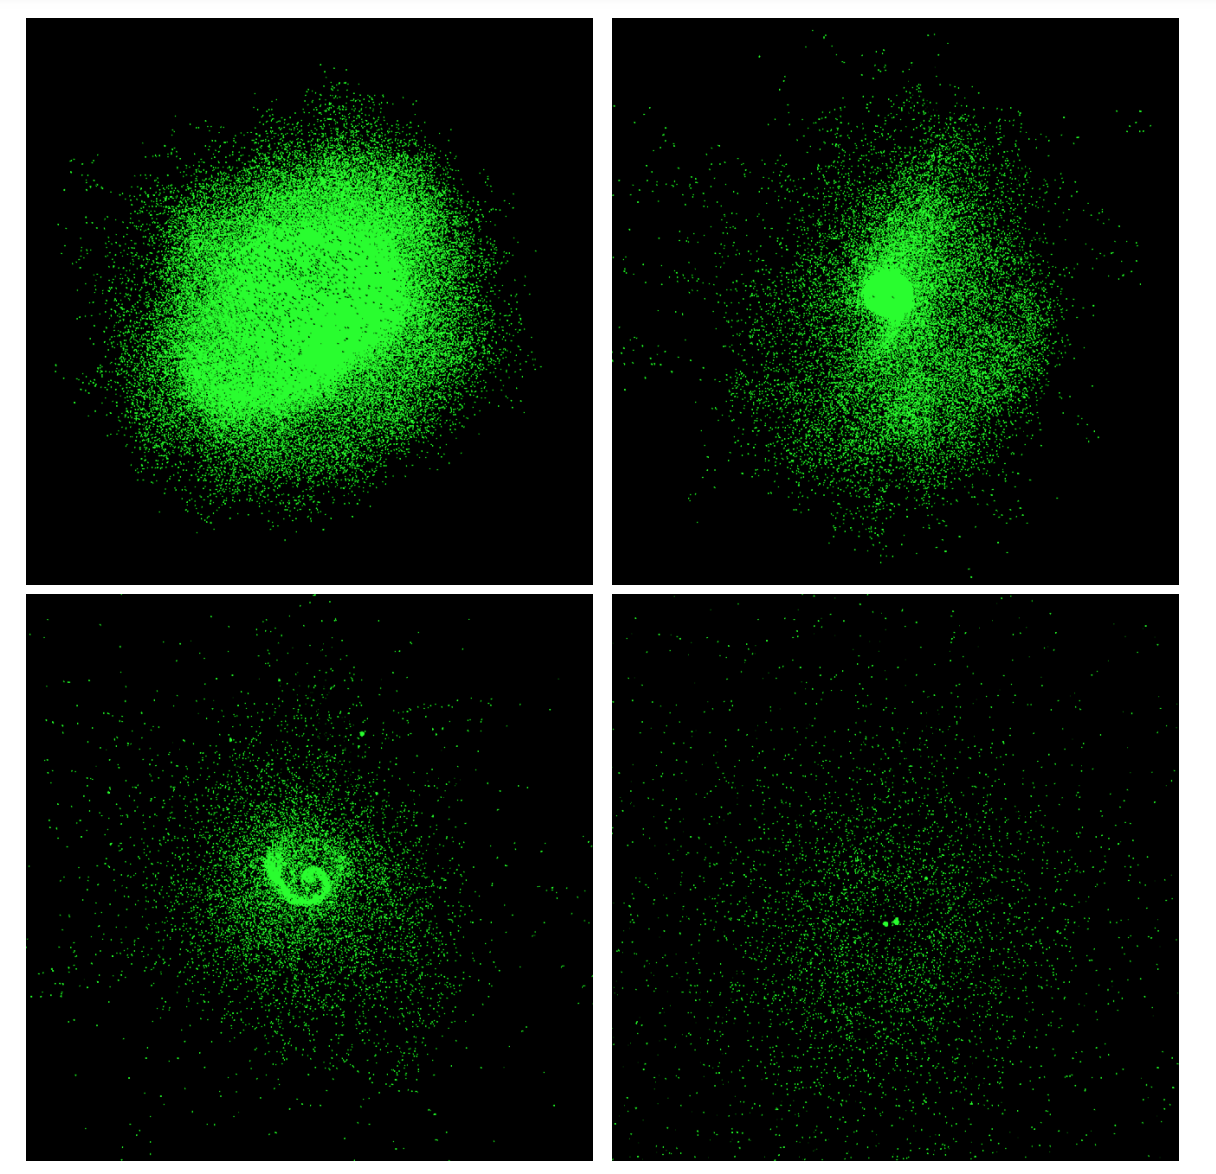
\includegraphics[width=\textwidth]{figures/intro/binaryPl.png}
    \caption{Simulation snapshots of a gravitationally bound pebble cloud formed via the streaming instability. Over the course of about 50 years (top left to bottom right), the clump collapses to form a binary planetesimal. (Adapted from figure 14 of \cite{nesvorny21})\label{fig:plCollapse}}
\end{center}
\end{figure}
 
Unfortunately, the conditions in simple models of protoplanetary disks are not sufficient to trigger the streaming instability. High resolution numerical studies suggest that dust to gas ratios larger than 4 percent are required to trigger it \cite{carrera15, yang17}, while the early solar system was thought to have a dust to gas ratio closer to 1 percent \cite{hayashi81}. This suggests that planetesimals should not be expected to form everywhere in the disk, although the fact that planets and smaller bodies, which presumably originated from planetesimals, exists everywhere from $\sim$ 0.5 to $\sim$ 50 AU in the solar disk. \textbf{It should be noted, that indirect measurements of the dust to gas ratio in planet forming disks exhibit a surprisingly wide range of values, some of which come close to the value required by streaming instability experiments \cite{rich21, jermyn22}.} Future, higher resolution studies of the streaming instability may \textbf{also} alleviate this discrepancy. \textbf{Another mechanism known as the vertical shear instability (VSI) \cite{urpin98} may provide an alternative pathway for the concentration of solids, although the exact midplane conditions that give rise to the VSI in a protoplanetary disk have not yet been well studied.}

Another solution to the problem of triggering the streaming instability may come from relaxing the assumption that the terrestrial planet forming regions of protoplanetary disks are smoothly varying. Pressure bumps in the gas disk, formed by mechanisms such as ionization fronts, condensation fronts, perturbations from other planets or self-induced dust traps \cite{gonzalez17} can all act to halt the inward drift of small solids and concentrate them into rings with conditions amenable to triggering the streaming instability \textbf{or} even gravitational fragmentation \textbf{\cite{chatterjee14, izidoro21, morbidelli21, batygin23a}}

\section{Observational Constraints}\label{sec:obsConstraints}

For $\mu$m to mm sized grains, scattered light from the central star, along with thermal emission allows us to directly trace this early phase of growth. For Earth-sized planets and larger, alterations to the light emitted by the host star allow us to observe the final outcome of the planet formation process. Populations of objects in between these sizes, however, do not have enough surface area to scatter light or emit appreciable amounts of thermal radiation, while being too small to perturb the light from the central star. With the exception of the remaining small bodies in the solar system, many of which are believed to be residual planetesimals, the gravitationally dominated stage of the terrestrial planet formation process is essentially invisible.

In the solar system, the orbital configurations of the planets themselves contain clues that the small body population was once much more numerous. A model in which the orbits of Saturn and Jupiter gradually evolve due to repeated scattering events with smaller bodies and subsequently go unstable works well to explain the present day configuration of the Jupiter trojans, Kuiper belt objects and irregular satellites \cite{gomes05, tsiganis05, morbidelli05,}. This suggests that the solar system was once filled with planetesimals. In addition, N-body simulations have shown that a collection 100 km sized objects placed throughout the outer solar system can induce the outward migration of Neptune's orbit while capturing the proper amount of small bodies into mean-motion resonance \cite{murrayclay06}.

For planet-forming disks around other stars, the primary way to infer the presence of planetesimals and planetary embryos is through dust emission. Although some of this dust is likely primordial, a large fraction of it is expected to be generated by collisions between the gravitationally bound planetary building blocks. Although the initial stages of planetesimal growth are not expected to create much dust, the eventual protoplanets that form act to stir up the remaining planetesimals, increasing collision velocities and producing destructive collisions \cite{kenyon04}. In 2020, the thermal emission of a transient dust cloud resulting from a planetesimal-planetesimal collision was observed for the first time \cite{gaspar20}.

\begin{figure}
\begin{center}
    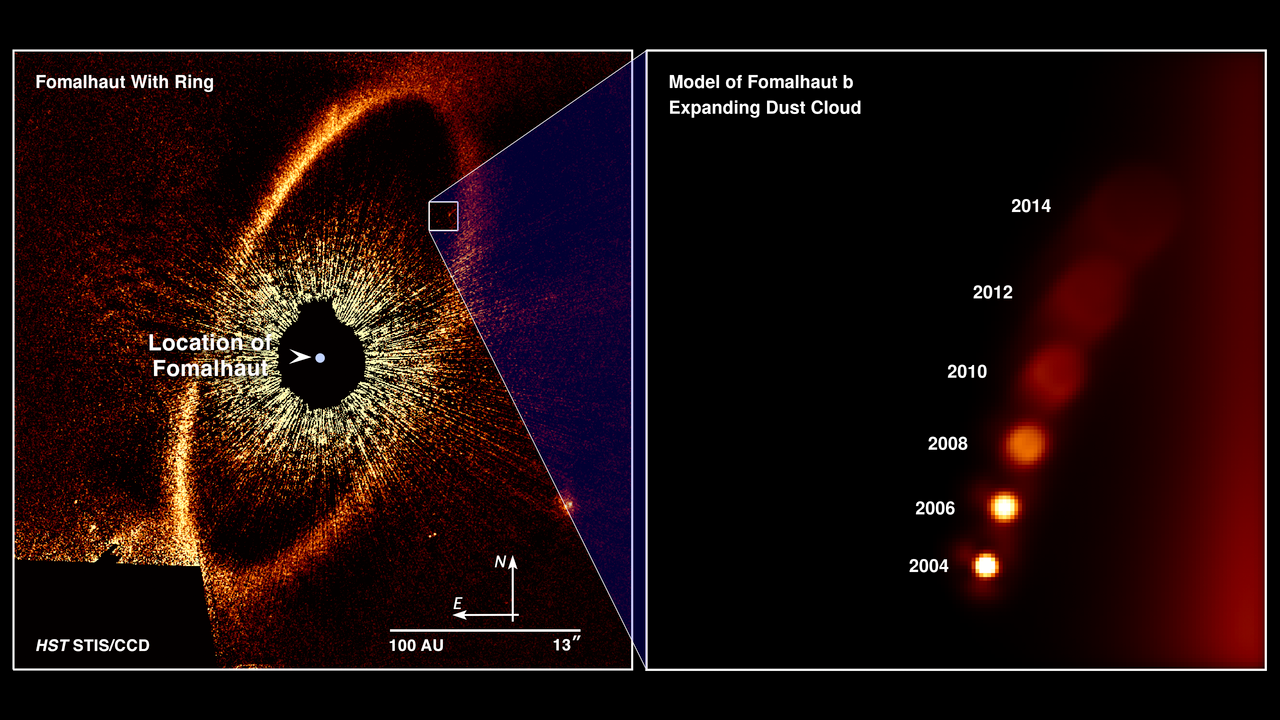
\includegraphics[width=\textwidth]{figures/intro/fomalhutb.png}
    \caption{A composite of archival images from the Hubble Space Telescope showing dust in scattered light surrounding the Fomalhut system. On the right, a closeup view of an expanding dust cloud, produced by a planetesimal collision is shown expanding over the course of 10 years. Image credit: NASA/ESA\label{fig:fomalhutb}}
\end{center}
\end{figure}

Often, the collisionally generated dust emission is used to infer the presence of an unseen planet. The intricate structure of bright rings and gaps seen in the planet-forming disk HL Tau \cite{alma15} have been argued to be indicative of three embedded giant planets \cite{boley17}. \cite{dobinson13, dobinson16} showed that the presence of a giant planet produces distinct morphological features in the collisionally generated dust emission, the properties of which can be used to constrain the orbital properties of the planet itself.

Despite powerful resolving capabilities ($\sim$ 1 AU resolution for the closest protoplanetary disks), sub-mm facilities like ALMA are not able to probe the terrestrial planet forming region of most disks. In fact, the inner 10 or so AU of most protoplanetary disks are optically thick at mm and shorter wavelengths \cite{beckwith90} and the conditions at the midplane where gravitationally bound solids are expected to form are completely hidden. Future radio observatories, such as the NG-VLA should be able to achieve sub-au resolution in the inner region of these disks \cite{ricci20}. In the meantime, constraints on planetesimal formation and terrestrial planet growth can only be attained by inward extrapolation of the solid distributions in the outer edges of observed protoplanetary disks, or by working backwards and reconstructing the conditions of the early solar system.

\section{Modeling Planetesimal Growth}

\subsection{Collision Rates and Runwaway Growth}

The problem of determining the outcome of planetesimal growth involves simultaneously evolving the mass distribution (as bodies collide and grow) and velocity distribution (as bodies gravitationally scatter) of the system. These models typically start with a collection of equal-mass planetesimals on nearly-circular, low inclination orbits about a much more massive central body. Predicting the evolution of the system requires a numerical approach, but some insights into the expected behavior can be obtained analytically. For an equal mass population of planetesimals with mass $m_{pl}$ and radius $r_{pl}$, the rate of change of the mass can be written as

\begin{equation}\label{eq:massgrow}
	\frac{dM}{dt} = \rho_{pl} v_{enc} \sigma = k \Sigma_{pl} \Omega \sigma,
\end{equation}

\noindent where $\rho_{pl}$ \textbf{and $\Sigma_{pl}$} is the mass \textbf{and surface density} density of planetesimals at the midplane of the disk, $v_{enc}$ is the typical encounter velocity between bodies, $\Omega$ is the Keplerian orbital frequency and $k$ is a numerical pre-factor which captures the geometric effects of encounters in a disk. The effective collision cross section $\sigma$ is set by the geometric value and is enhanced by gravitational focusing \cite{safronov69}, which bends the trajectories of planetesimals that undergo a close encounter.

\begin{equation}\label{eq:gf}
	\sigma = \pi r_{pl}^2 \left( 1 + \frac{v_{esc}^2}{v_{enc}^2} \right),
\end{equation}

\noindent where $v_{esc}$ is the mutual escape velocity of two planetesimals that are in contact at their surfaces.

In the case where the planetesimal disk is dynamically cold ($v_{esc} \gg v_{enc}$), equation \ref{eq:massgrow} scales with mass as $dM/dt \propto M^{4/3}$. This implies that the growth rate accelerates with time and leads to a situation known as runaway growth \cite{wetherill89, kokubo96}.

\subsection{Two-body Relaxation}

At the same time, the encounter velocities in the disk evolve due to two-body relaxation. This is effectively due to gravitational encounters converting energy from the differential rotation of the disk into random motion. For an equal mass population of bodies, the timescale for relaxation can be written as 

\begin{equation}\label{eq:relax}
	t_{relax} = \frac{v_{enc}^2}{d v_{enc}^2 / dt} = \frac{v_{enc}^3}{\rho_{pl}^2 \pi G^{2} m_{pl}^4 ln \Lambda}
\end{equation}

\noindent where $G$ is the gravitational constant and $ln \Lambda$ is the Coulomb logarithm, which captures the effects of long-distance encounters and is typically taken to be $\simeq$ 10 for a planetesimal disk.

As the planetesimal system evolves, the assumption of equal-mass bodies is quickly violated. In this situation, a numerical approach is required. This was first done by \cite{greenberg78} and involves dividing growing planetesimals into bins of mass and distance from the central star and evolving them using a statistical approach. This method, which provided the first confirmation that runaway growth indeed persists beyond the initial equal-mass phase \cite{wetherill89}, suffers from a few severe limitations. First, dynamical effects such as energy exchange between bodies of different masses and encounters between slow-moving bodies which are strongly mediated by the gravitational field of the central object, must be explicitly built in to the model. Second, runaway growth naturally produces a power law tail of bodies. In this situation, the highest mass bins eventually end up with only a few bodies which dominate the dynamical evolution of the system and a statistical approach begins to break down.

\subsection{N-body Simulations of Planetesimal Accretion} \label{sec:nbodyPl}

The straightforward, albeit computationally expensive way to circumvent these problems is to instead evolve the equations of motion for the growing planetesimals individually. To do so explicitly requires pairwise force evaluations and collision checks between all bodies at every timestep. Given that these calculations naively require $O(n^2)$ evaluations per timestep, this can quickly become prohibitively expensive, especially considering that terrestrial planet formation timescales are on the order of Myrs, while dynamical timescales between planetesimals can be on the order of days. It took decades after the idea of runaway growth was first proposed before its effects and eventual end were directly simulated using an N-body code \cite{kokubo96, kokubo98}. Even then, the simulations were limited to a narrow annulus, where it was assumed that the growth modes scaled in a self-similar way throughout a full planetesimal disk.

The introduction of tree-based N-body codes such as {\sc pkdgrav} \cite{richardson00, stadel01, wadsley04} finally allowed for much larger particle counts to be used, in which planetesimals were much closer to the sizes predicted by formation models. By dividing physical space into subdomains, force calculations and neighbor lookups for collision detection can be done in $O (n log n)$ time using an algorithm similar to a Barnes-Hut tree \cite{barnes86}. 

The simulation code used to model planetesimal accretion in this thesis is called {\sc ChaNGa}, which is a descendent of {\sc pkdgrav}. {\sc ChaNGa} is actively being developed by the N-body shop at the University of Washington and is designed to enable force calculations and neighbor finding for huge collections of particles by efficiently distributing the work across machines running in parallel on a supercomputing cluster \cite{jetley08, menon15}. This is done by splitting groups of particles into objects called TreePieces, which are then assigned to different compute domains and are designed so that calculations on a given TreePiece can be done semi-independently. \textbf{Because neighboring particles can sometimes end up in different TreePieces, remote data can be accessed during a tree walk using a cache manager, which acts to minimize unnecessary communication and waiting \cite{menon15}.} Much of the power of {\sc ChaNGa} comes from the fact that load balancing and communication between cores is handled in a very dynamic and efficient way. For cosmological simulations, {\sc ChaNGa} can easily handle upwards of billions of particles, although the much larger range of timescales that must be handled in a planetesimal accretion simulation restricts this to a few million.

{\sc ChaNGa} is written in the {\sc CHARM++} programming language and has been shown to perform well when using up to half a million processors \cite{menon15} simultaneously. Gravitational forces are calculated using a modified Barnes-Hut tree algorithm with hexadecapole order expansions of the moments. For all of the planetesimal accretion simulations described in this paper, a node opening criterion of $\Theta_{BH}$ = 0.7 was used. In chapter \ref{ch:plSS}, I test the effects of varying $\Theta_{BH}$ on a planetesimal disk and show that the tree approximation does not meaningfully affect the influence of two-body encounters. The equations of motion are integrated using a kick-drift-kick leapfrog scheme. For more information about the implementation of {\sc ChaNGa} see \cite{jetley08}.

In order to use {\sc ChaNGa} to study planetesimal coagulation, I implemented a hard-body collision model that treats particles as solid objects with a fixed radius, rather than as smooth tracers of a fluid with a characteristic softening length. The framework for the collision detection module uses the existing algorithm for neighbor finding during smooth particle hydrodynamics (SPH) calculations. As with the gravity calculations, particles are sorted into a tree structure which allows the collision search to be conducted in $\mathcal{O}(N\log{}N)$ time. The collision detection module in {\sc ChaNGa} based off of the solid body collision implementation in {\sc pkdgrav}, which is described in \cite{richardson94} and \cite{richardson00}, which we summarize below:

Collisions are predicted at the beginning of each drift step by extrapolating the positions of the particles forward using the velocities calculated during the first kick. For each particle, the closest 64 neighbors are considered in the collision search. After extrapolating the positions forward and checking for overlap with any neighbors, the earliest collision time $t_{coll}$ is stored for each particle.

After the prediction phase, particles with $t_{coll}$ less than the time step size $\Delta T$ must have their collisions resolved. For simplicity, all collisions in our simulations result in perfect accretion. A merger between two particles of mass $m_{1}$ and $m_{2}$ results in a single particle of mass $M = m_{1} + m_{2}$, with the radius set to conserve density. The position and velocity of the resulting particle is set to the centre of mass position and velocity of the colliders at the moment of contact. The resulting merged particle is then drifted to the end of the step. If multiple collisions are predicted during a time step, the earliest collision is resolved first. Because resolving a collision can result in another imminent collision, collisions must be resolved one by one, with a new prediction check being run each time.

\subsection{N-body Simulations of Final Planet Assembly}

Although tree-based N-body codes work well for modeling planetesimal accretion, the later stages of terrestrial planet formation, in which protoplanets collide to form planets, requires integrating through prohibitively large number of dynamical times (on order $10^{10}$ timesteps). During this phase, collisions and close gravitational encounters are rather infrequent. During timesteps where there are no close encounters, a mixed variable symplectic \textbf{(MVS)} integration scheme can be used \cite{wisdom91}. This involves splitting the Hamiltonian of a system into a Keplerian and perturbing part. \textbf{Although all particles induce perturbations on each other} these two parts can be solved independently, \textbf{so long as the perturbations are small. The Keplerian part of the Hamiltonian can be solved analytically, allowing for much larger timesteps compared with} solving the equations of motion using a direct $O(n^{2})$ or a tree-based approach. In cases where a close encounter occurs, the perturbing term in the Hamiltonian becomes large and the motion of the interacting particles is solved directly. This hybrid integration scheme was first implemented in the code {\sc Mercury} \cite{chambers99} and allowed for the first time planet formation simulations using hundreds to thousands of particles.

Restricting planet formation simulations to begin with no more than a few thousand particles, is still quite limiting. Due to this restriction, these types of simulations are often built with rather unrealistic initial conditions, in which planetary embryos are already fully formed in the disk and residual planetesimals are either represented by super-particles, or their gravitational influence is ignored. Recent advances in GPU hardware, however, have allowed more recent N-body codes to push beyond these limitations. In particular, the N-body code {\sc genga} \cite{grimm14, grimm22} has been developed to specifically take advantage of GPU hardware for running a hybrid MVS integrator up to 30 times faster than {\sc Mercury}. Recent versions of {\sc genga} are able to efficiently handle prolonged close encounters between large groups of particles and the code has been successfully used to model the coalescence of tens of thousands of fully self-interacting particles into a system of terrestrial planets \cite{woo21}.

\section{Thesis Goals and Outline}

In this thesis, I present my work using high resolution N-body simulations to understand the dynamics and outcome of the planetesimal accretion process. I will begin by connecting this process to the present-day small body populations in the inner solar system, particularly the asteroid belt. Then, I examine the role that planetesimal collisions play in the generation of debris disks. Lastly, I follow the growth of a planetesimal disk into a fully-formed system of short-period planets. From here, I make connections with the compact, multiplanet systems observed by Kepler and TESS to understand how viable a migration-free terrestrial planet formation model can be in this context.

\subsection{Chapter 2 Summary}

In chapter 2, I revisit the problem of planetesimal accretion in the inner solar system starting with near-realistic sized bodies. I show that the post-runaway growth phase is resolution dependent and that finely-spaced mean-motion resonances with the largest bodies are only populated if the planetesimal population is sufficiently fine-grained. In the case where this condition is met, the mass distribution of the residual planetesimal population follows a broken, rather than a single power law. This is strongly reminiscent of the mass distribution of the present day asteroid belt and Kuiper belt and I demonstrate that subsequent collisional destruction is not the only pathway to produce such a break.

\subsection{Chapter 3 Summary}

In chapter 3, I follow the orbital evolution of a planetesimal belt in the vicinity of a giant planet and use the recorded collision rates to construct a dust emission map. Near the locations of mean-motion resonances, distinct overdensities or underdensities in the dust can form. The mapping between particular resonances and the presence of a gap or bright ring in the dust emission is shown to depend on the mass and eccentricity of the giant planet. I show that from the dust emission alone, it is possible to constrain the orbital properties of the giant planet.

\subsection{Chapter 4 Summary}

In chapter 4, I simulate the planetesimal accretion process at short (1 to 100 day) orbital periods and show that the gravitational interactions that facilitate energy equipartition and eventually shut off the runaway growth phase become ineffective close to the star. I show that a disk of rocky planetesimals should be expected to undergo two distinct accretion modes, with the boundary lying around 5 to 10 days in orbital period. This result has implications for the expected configuration of planetesimals and embryos at the beginning of the giant impact phase and suggests that the initial conditions used for short-period planet formation simulations are often overly simplistic. In the following chapter, I use these simulation results to explore the effect that this accretion boundary in the disk has on the final assembly of the planets.

\subsection{Chapter 5 Summary}

In chapter 5, I use the final simulation snapshots from chapter 4 to grow the remaining planetesimals and protoplanets into a fully-formed system of terrestrial planets under a migration-free model. These are the first-ever simulations in which the planet formation process is followed from the smallest gravitationally bound bodies (planetesimals) to full-sized planets. Having directly resolved every collision, I map the building blocks of the planets back to their original locations in the disk to assess the extent of radial mixing in the disk. Due to the computational expense of the planetesimal accretion simulations, I train a neural network on the results from the previous chapter and use it to produce a much larger set of intermediate-phase initial conditions which are then run and used to capture the effects of stochasticity and chaos during the giant impact phase.

\chapter {Formation of Planetary Embryos in the Inner Solar System}\label{ch:plSS}

\noindent \textit{The content of this chapter was originally published in collaboration with Thomas R. Quinn in the October 2019 edition of The Monthly Notices of the Royal Astronomical Society (\cite{wallace19}, MNRAS, Vol. 489, 2; 2019, DOI: 10.1093/mnras/stz2284/), and is reproduced below with the permission of the Royal Astronomical Society.}

\section{Introduction} \label{sec:intro}

The standard scenario of terrestrial planet formation involves the pairwise accretion of small rocky bodies, called planetesimals, 
that condense from dust out of the protostellar disc \cite{safronov69}. \textbf{As discussed in chapter \ref{ch:intro}, the details of growth from cm to km sizes remains uncertain due to fragmentation, bouncing and radial drift barriers \cite{windmark12, weidenschilling77}. However, instabilities that produce large local concentrations of dust and pebbles may provide a way to circumvent these problems \cite{urpin98, youdin05, squire18, squire20}. Assuming larger solids do eventually form, gravity begins tho dominate the physics for objects around a hundred km in diameter.}

\textbf{At this point, gravitational focusing \cite{safronov69} drives runaway growth \cite{duncan89, kokubo96, barnes09} and a handful of relatively large bodies develop. At this point, the largest bodies known as oligarchs, scatter the remaining planetesimals and act to slow the runaway effect. Eventually, the oligarchs accrete most of the available material in the vicinity of their orbit, and space themselves apart by approximately 5-10 Hill radii \cite{kokubo98, kokubo02}. On much longer time scales, the large bodies perturb each other onto crossing orbits, forming Mars to Earth sized bodies via occasional collisions. This phase of late stage accretion is highly chaotic and takes much longer to play out than the previous stages \cite{chambers98, raymond06}.}

%The standard scenario of terrestrial planet formation involves the pairwise accretion of small rocky bodies, called planetesimals, 
%that condense from dust out of the protostellar disc \cite{safronov69}. This accretion process can be broken into a series of 
%distinct stages. First, dust particles settle toward the midplane of the disc and clump together via gravitational instability 
%\cite{goldreich73, youdin02}, streaming instabilities \cite{johansen07, johansen15}, turbulent concentration 
%\cite{chambers10, cuzzi08, cuzzi10, hopkins16} or direct sticking \cite{okuzumi12, windmark12, garaud13, katoka13}. These 
%formation models predict a wide variation in the initial size of planetesimals, ranging from hundreds of meters up to a few 
%hundred kilometers in diameter.

%After this condensation process ends, growth continues via pairwise collisions between planetesimals. Above about 1 km in size, 
%gravitational focusing becomes effective and the collision rate strongly increases. This marks the beginning of the intermediate 
%stage of accretion. During this phase, runaway growth \cite{duncan89, kokubo96, barnes09} quickly increases the size of the 
%largest bodies. Eventually, the largest bodies grow massive enough to heat the small planetesimals, which then inhibits the 
%runaway growth effect. This marks the transition into the phase of oligarchic growth in which the handful of large bodies all tend 
%to grow at the same rate. This produces a bimodal size distribution of planetesimals, with many small bodies and a handful of 
%very large bodies. During this phase, a combination of scattering events between the oligarchs and dynamical friction from the 
%small planetesimals places the oligarchs on nearly circular orbits that are spaced apart by approximately 5-10 Hill radii 
%\cite{kokubo98}. Eventually, the oligarchs accrete most of the available material in the vicinity of their orbit, which eventually 
%throttles their growth rate. On much longer time scales, the large bodies perturb each other onto crossing orbits, forming Mars to 
%Earth sized bodies via occasional collisions. This phase of late stage accretion is highly chaotic and takes much longer to play 
%out than the previous stages \cite{chambers98, raymond06}.

Generally, planetesimal accretion models fail to produce a configuration of planets that resembles that of the Solar System. 
Planets produced in the vicinity of Mars are systematically too massive \cite{wetherill92, raymond09, morishima10, izidoro15} 
and the terrestrial planets that form are too eccentric compared to their Solar System counterparts 
\cite{chambers98, agnor99, chambers01}. In addition, the present day water content of Earth, along with the large D/H ratio of 
Venus \cite{donahue82} does not match with models of solids that condensed out of the Solar nebula at 1 AU.

These issues all have proposed solutions, which generally involve altering the initial conditions for late-stage
accretion simulations. The condition of the Solar System at the beginning of the late stage accretion phase is poorly constrained. 
This is mostly due to the fact that planetesimal formation, and therefore the intermediate accretion phase which produces the 
planetary embryos, is not well understood. Although the present day population of small Solar System bodies has continued to 
evolve since the end of the intermediate accretion phase, the current size frequency distribution (SFD) of asteroid belt and 
Kuiper belt objects contains some clues about the accretion history. \cite{morbidelli09} argued that the SFD of asteroid belt 
objects larger than 100 km in diameter has been largely unchanged, aside from a size independent depletion factor. 
\cite{duncan89} did a long term stability analysis of small Solar System objects and found that small bodies left over from 
accretion should still be largely unperturbed. For these reasons, it should be possible to connect observables in the Solar System to planetesimal formation theories by modeling only the intermediate stages of accretion.

%There are two common ways to model planetesimal growth. A powerful approach is to use statistical methods to track the 
%evolution of large groups of planetesimals. This is known as the particle-in-a-box method \cite{greenberg78, wetherill89}. The 
%evolution of growth is followed by tracking planetesimals in discrete bins of mass and semi-major axis. This removes the need to 
%calculate the motion of every individual body and allows very large collections of planetesimals to be followed. Unfortunately, the 
%dynamics that governs the evolution of these bodies does not always naturally emerge with this approach. 
\textbf{Statistical methods \cite{greenbern78, wetherill89} have proven to be a powerful approach to model planetesimal growth. However, the dynamics governing the evolution of growing planetesimals and protoplanets does not always naturally emerge with this technique.} As an example, 
\cite{weidenschilling11} found that a careful treatment of three body encounters led to a different prediction for the initial size 
distribution of planetesimals near the asteroid belt. Additionally, the particle-in-a-box method is not well suited for studying 
oligarchic growth because the largest mass bins, which dominate the evolution in this stage, contain small numbers of bodies. 
Non-gravitational effects such as gas drag and fragmentation require extra care to implement self-consistently 
\cite{leinhardt08}, although it has been successfully done \cite{wetherill93, chambers01}. To alleviate some of these issues 
while still being able to model large populations, a newer hybrid approach, in which large bodies are treated as single entities 
and planetesimals are treated as statistical ensembles has been developed 
\cite{weidenschilling97, kenyon06, levison12, morishima15}.

The most reliable and straightforward approach is to use N-body methods to follow the evolution and growth of the planetesimals 
\cite{lecar86}. By tracking the individual motions of bodies, the dynamics governing their evolution naturally emerges, no matter 
what the distribution of bodies looks like. However, N-body simulations involving collision detection are extremely 
computationally expensive, which severely limits both the resolution and number of timesteps that can be achieved. This is why 
there are very few studies of runaway and oligarchic with direct N-body simulations in the literature 
\cite{kokubo96, kokubo98, kokubo02, barnes09}. Instead, N-body methods are most commonly used to study late stage 
accretion, where the self-gravity and collisional evolution of the residual planetesimals is largely unimportant 
\cite{chambers98, agnor99,  chambers01, obrien06, morbidelli09}.

To date, we are not aware of any N-body simulations that resolve both the runaway and oligarchic growth phase  with more than 
about $10^4$ particles. At this resolution, stochasticity likely has a significant influence on dynamical friction and resonances 
may not be sufficiently resolved. \cite{raymond06} found that insufficient planetesimal resolution during the oligarchic growth 
phase limits the effectiveness of dynamical friction felt by the oligarchs, producing a population of embryos with unrealistically 
high eccentricities. This idea has also been applied to planet migration through a disc of planetesimals. \cite{cionco02} showed 
that resonances make a significant contribution to the dynamical friction torque exerted by the disc on the planet. This 
phenomenon requires the planetesimals to be finely resolved \cite{brunini07}. Dynamical friction is also facilitated via 
resonances in galactic dynamics \cite{lyndenbell72}. \cite{weinberg07a, weinberg07b} examined the effect of N-body particle 
counts on galaxy dynamics and showed that resonant interactions between the bar and halo were only effective with sufficient 
particle phase space coverage.

For these reasons, we motivate the need for a high resolution N-body simulation of planetesimal growth. We do this to better 
understand the effect that dynamical friction has on the intermediate stages of terrestrial planet growth and to examine what 
predictions a high resolution model makes about the residual population of planetesimals in the Solar System. In particular, 
resonances which are only effective with fine enough resolution, may have an important influence on planetesimal growth. In this 
chapter, we investigate planetesimal evolution during the runaway and oligarchic growth phases with a direct N-body model. We 
begin by simulating an annulus of planetesimals with similar resolution to \cite{kokubo98} to validate our model. We then run the 
same configuration with 100x more particles to better understand the effects of resolution on the intermediate stages of 
terrestrial planet growth.

In section \ref{sec:sim}, we provide a summary of the simulation code, along with a description of the initial conditions used.
In section \ref{sec:plSS_results}, we present the results of the low and high resolution 
simulation of terrestrial planet growth and highlight differences between the two. We find that a bump develops in the mass 
distribution of the high resolution simulation, which does not appear in the low resolution run. This feature manifests itself shortly 
after oligarchic growth commences and we infer that it is produced by extra heating via mean motion resonances between the 
oligarchs and small planetesimals. To further demonstrate this effect, we re-run the high resolution simulation with a narrower 
annulus (depopulating many of the resonances) and show that this reduces the prominence of the bump in the mass distribution. 
In section \ref{sec:dynfric}, we present a set of collisionless simulations of a planetary embryo embedded in an annulus of 
planetesimals. This more clearly demonstrates the differences in dynamical behavior between the low and high resolution 
models. In section \ref{sec:intermed}, we present two more simulations of planetesimal growth at intermediate resolutions and 
demonstrate that the location of the bump is sensitive to the initial planetesimal mass. Finally, section \ref{sec:discussion} 
connects these new results to our present understanding of terrestrial planet growth and we discuss the additional steps 
necessary to use our results to constrain the initial size of planetesimals in the Solar System.

\section{Simulations} \label{sec:sim}

\subsection{Numerical Methods} \label{sec:numerical}

All of the simulations described in this chapter were performed with the highly parallel N-body code {\sc ChaNGa}. A full description 
of the code, along with the details of the solid body collision module are provided in chapter \ref{ch:intro}. For all of the simulations 
presented below, we use a node opening criterion of $\Theta_{BH} = 0.7$. In section \ref{sec:openAngle}, we reduce the value of 
$\Theta_{BH}$ and show that a more accurate and expensive force calculation does not meaningfully affect the timescale for 
viscous stirring.

As in \cite{kokubo96, kokubo98} we accelerate the accretion process by artificially inflating the physical radius of the bodies by 
a factor of $f$. This technique reduces the accretion time-scale by approximately a factor of $f^{2}$, significantly reducing the 
number of timesteps that must be integrated. Additionally, inflating the particle radii allows us to use a smaller annulus with less 
planetesimals. The reason we cannot use an arbitrarily skinny annulus is because the edges tend to expand outward due to the 
unrealistic boundary conditions, decreasing the surface density. The time-scale for this expansion is set by the two body 
relaxation time-scale, which scales with $N$. Reducing the accretion time-scale by increasing $f$ allows us to study 
planetesimal growth with a smaller, less computationally expensive annulus.

We must be careful, however, to choose a value of $f$ that is not too large. The rms eccentricity and inclination of the 
planetesimal disc grows as gravitational encounters transform energy due to Keplerian shear into random motions. By 
accelerating the growth rate, we cause the transitions between growth modes to happen early, when the disc is less dynamically 
excited. This discrepancy is partly compensated for by the fact that our model ignores the effects of gas drag, which would damp 
the eccentricities and inclinations of the planetesimals. We adopt $f=6$ for our calculations, which reduces the amount of 
gravitational scattering by less than 10\% of its true value and does not qualitatively change the modes of planetesimal growth 
\cite{kokubo98}.

\subsection{Initial Conditions} \label{sec:ics}

We begin by using our collision model to perform two sets of calculations:

(i) $10^{6}$ equal mass bodies with $m = 1.2 \times 10^{21}$ g

(ii) 4000 equal mass bodies with $m = 3 \times 10^{23}$ g

\noindent As previously mentioned, simulation (ii) is meant to be compared with the results of \cite{kokubo98}. This allows us to 
both validate our collision model and also have a baseline to compare our simulations to. In both cases, the planetesimals are 
distributed randomly in an annulus centred at 1 AU with a width $\Delta a = 0.085$ AU around a 1 $\mathrm{M_{\odot}}$ star. 
This annulus width was chosen so that the required particle count is minimized without boundary effects influencing planetesimal 
growth. The surface mass density of the ring is set to 10 g cm$^{-2}$, which approximately corresponds to the minimum-mass 
solar nebula model \cite{hayashi81} at 1 AU. In case (i), the eccentricities and inclinations are taken from a Rayleigh distribution 
\cite{ida92} with $\langle e^2 \rangle^{1/2} = 2 \langle i^2 \rangle^{1/2} = 4 h/a$, where $h$ is the mutual Hill radius. To match 
the same eccentricity and inclination dispersion with larger planetesimals in case (ii), we use $\langle e^2 \rangle^{1/2} = 2 
\langle i^2 \rangle^{1/2} = 0.635 h/a$. In both simulations, the planetesimals are given an internal density of 2 g cm$^{-3}$. We 
use fixed timesteps with $\Delta T$ = 0.0025 years and evolve the simulations for 20,000 years. Large timesteps diminish the 
effectiveness of gravitational focusing, which inhibits the collision rate. We find that the collision rate is converged below $\Delta 
T$ = 0.0025 years. The integration time was chosen to be comparable to the orbital repulsion and Hill radius growth time-scale 
\cite{kokubo95} so that the effects of oligarchic growth are fully realized by the end of the simulation.

It is worth noting that simulation (i) was a very computationally expensive undertaking. In total, the full 20,000 years of 
integration required approximately 130,000 CPU hours and over 50 days of wall clock time.

\begin{figure}
    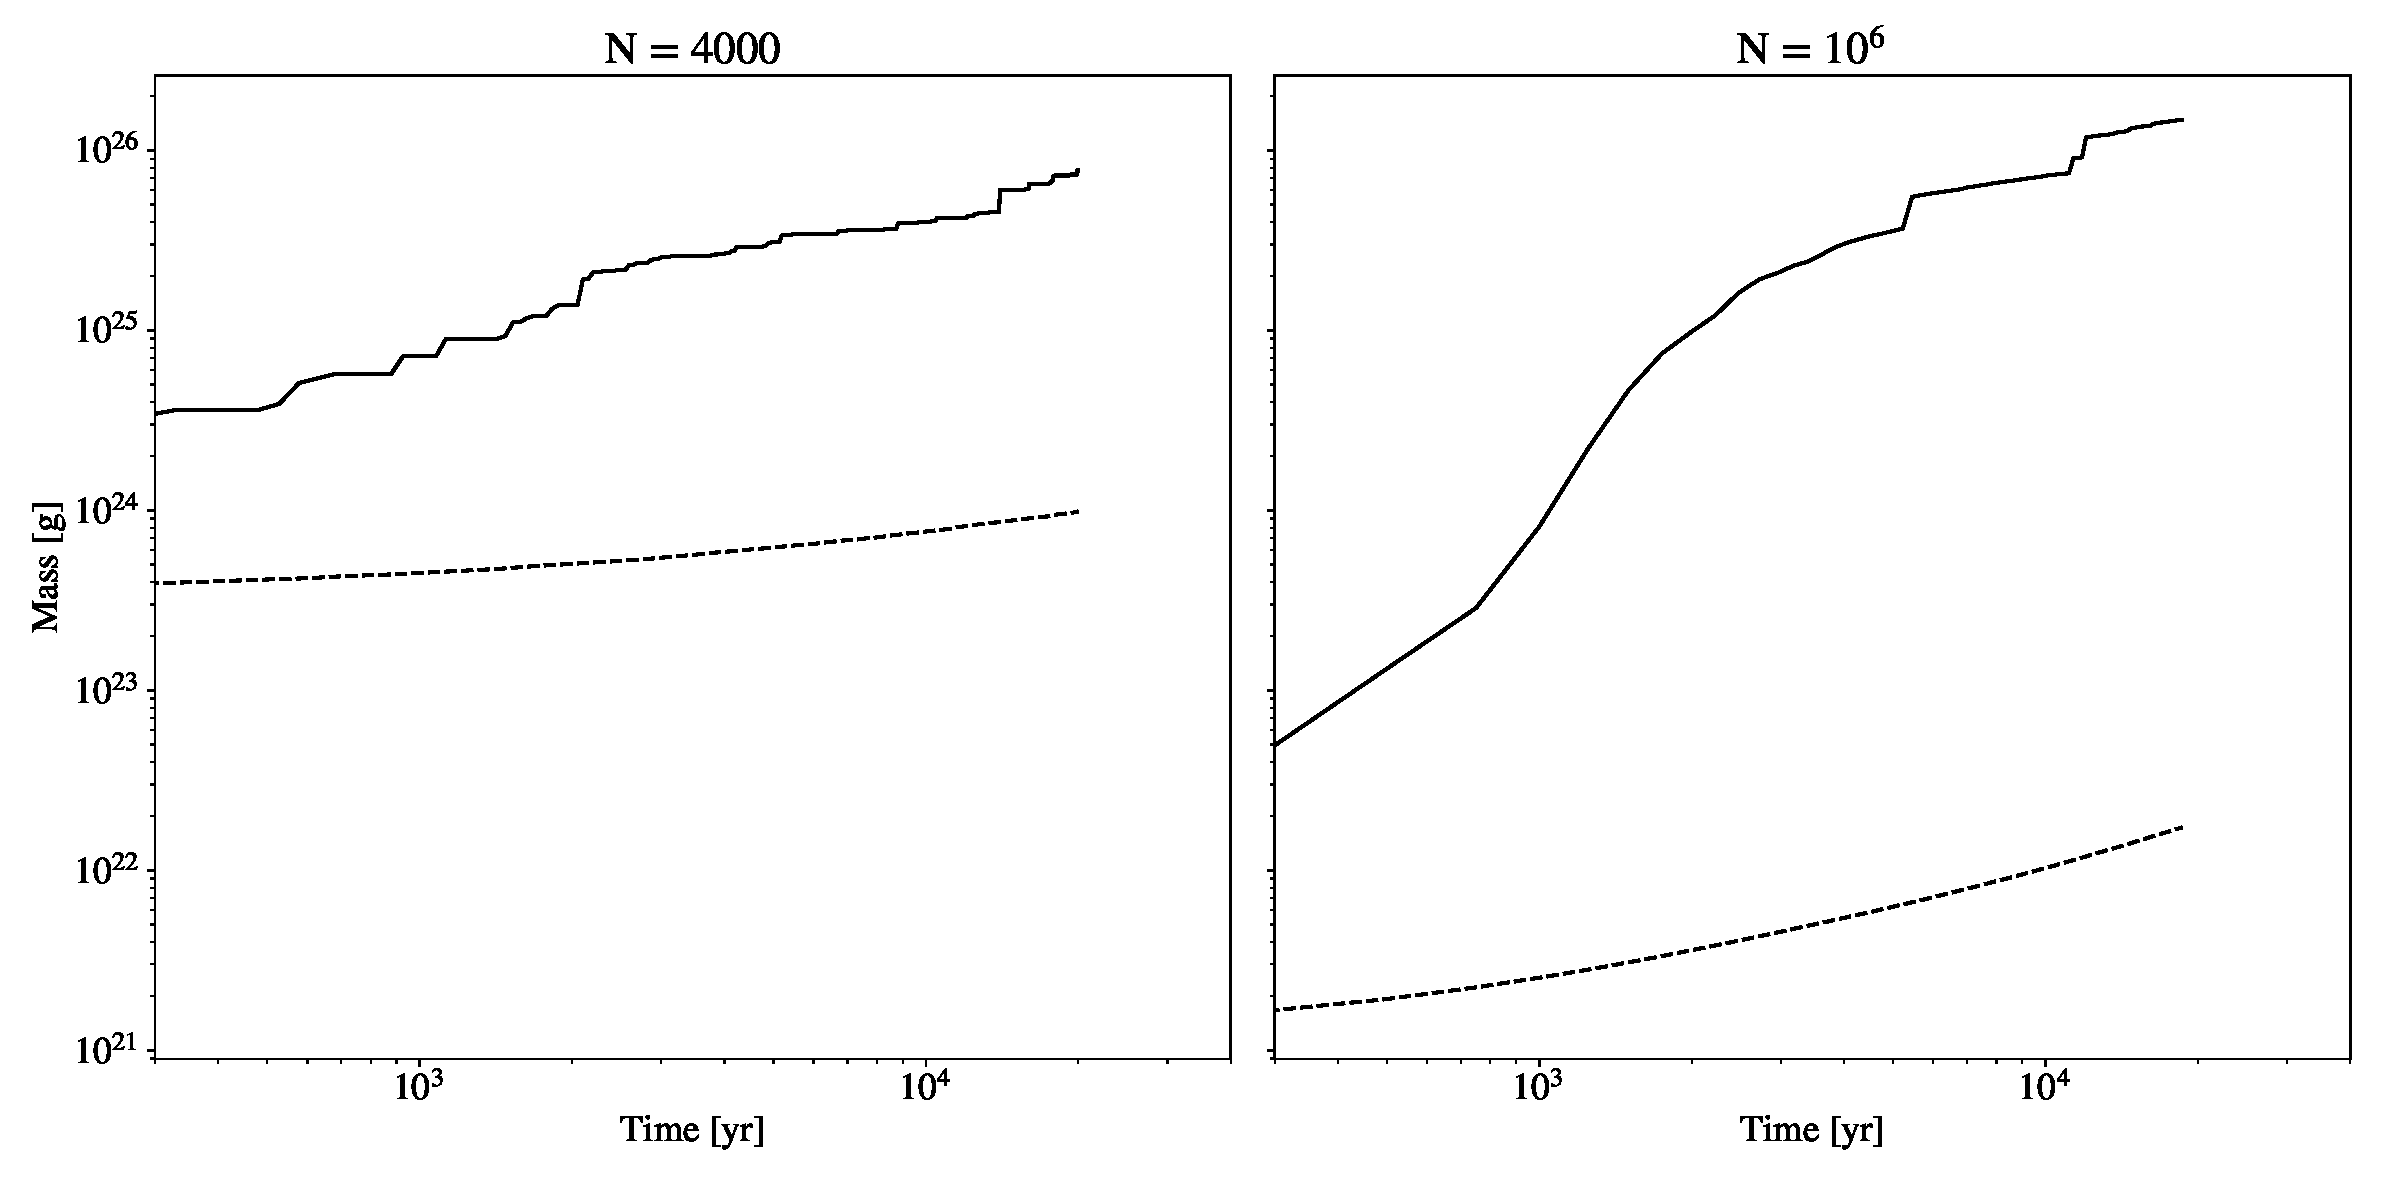
\includegraphics[width=\textwidth]{figures/plSS/mass_evo.eps}
    \caption{Evolution of the maximum (solid curve) and mean (dashed curve) planetesimal mass in the N=4000 and N=$10^6$ particle simulations. At early times, the maximum mass grows more quickly than the mean mass, which is indicative of runaway growth. After a few thousand years, the separation between the curves becomes a constant factor, signalling the start of oligarchic growth.
    \label{fig:mass_evo}}
\end{figure}

\begin{figure}
    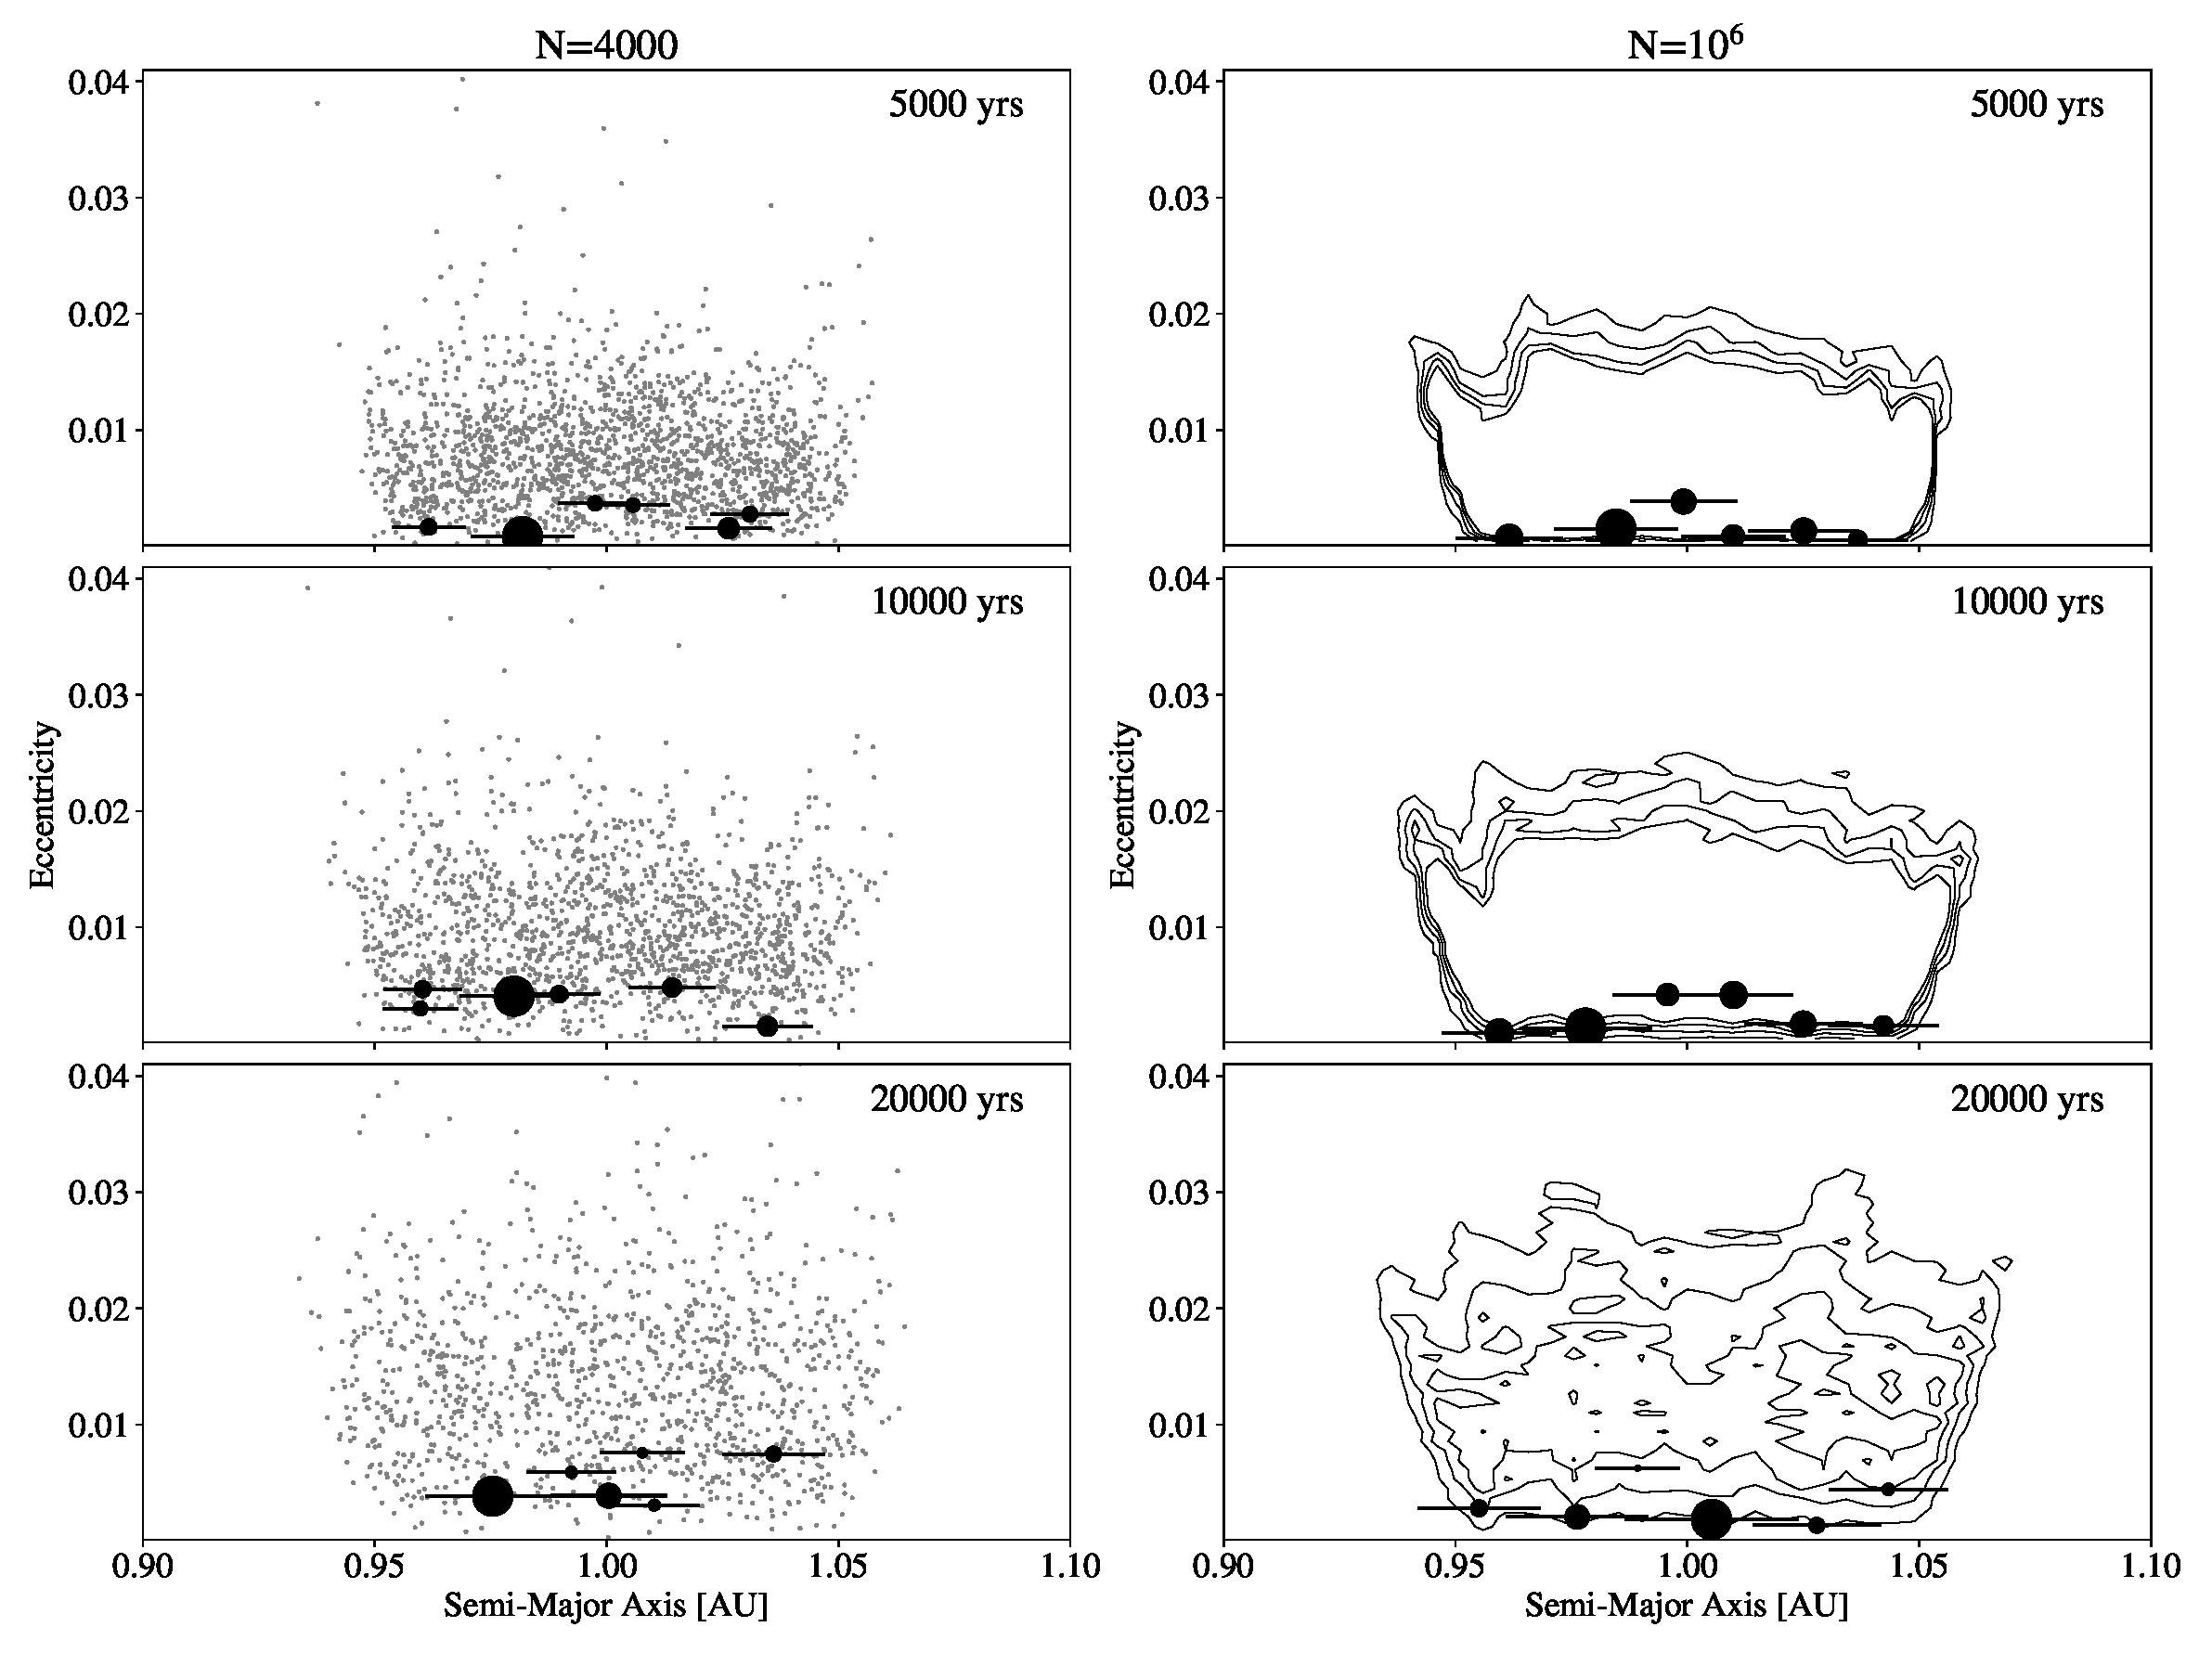
\includegraphics[width=\textwidth]{figures/plSS/ecc_evo.eps}
    \caption{Snapshots from the low and high resolution models in the $a-e$ plane. On the left, the light dots represent individual planetesimals, while the contours on the right hand plots represent curves of constant number density. The contour levels are the same between all panels and correspond to $7.8 \times 10^6$, $1.6 \times 10^7$, $2.3 \times 10^7$, and $3.1 \times 10^7$ planetesimals per AU per unit eccentricity. The black circles denote the configuration of the 6 largest bodies in the simulation, with the area of the circles scaled to the mass of the body. The horizontal error bars are scaled to 5 times the Hill radius of the bodies.
    \label{fig:ae}}
\end{figure}

\begin{figure}
    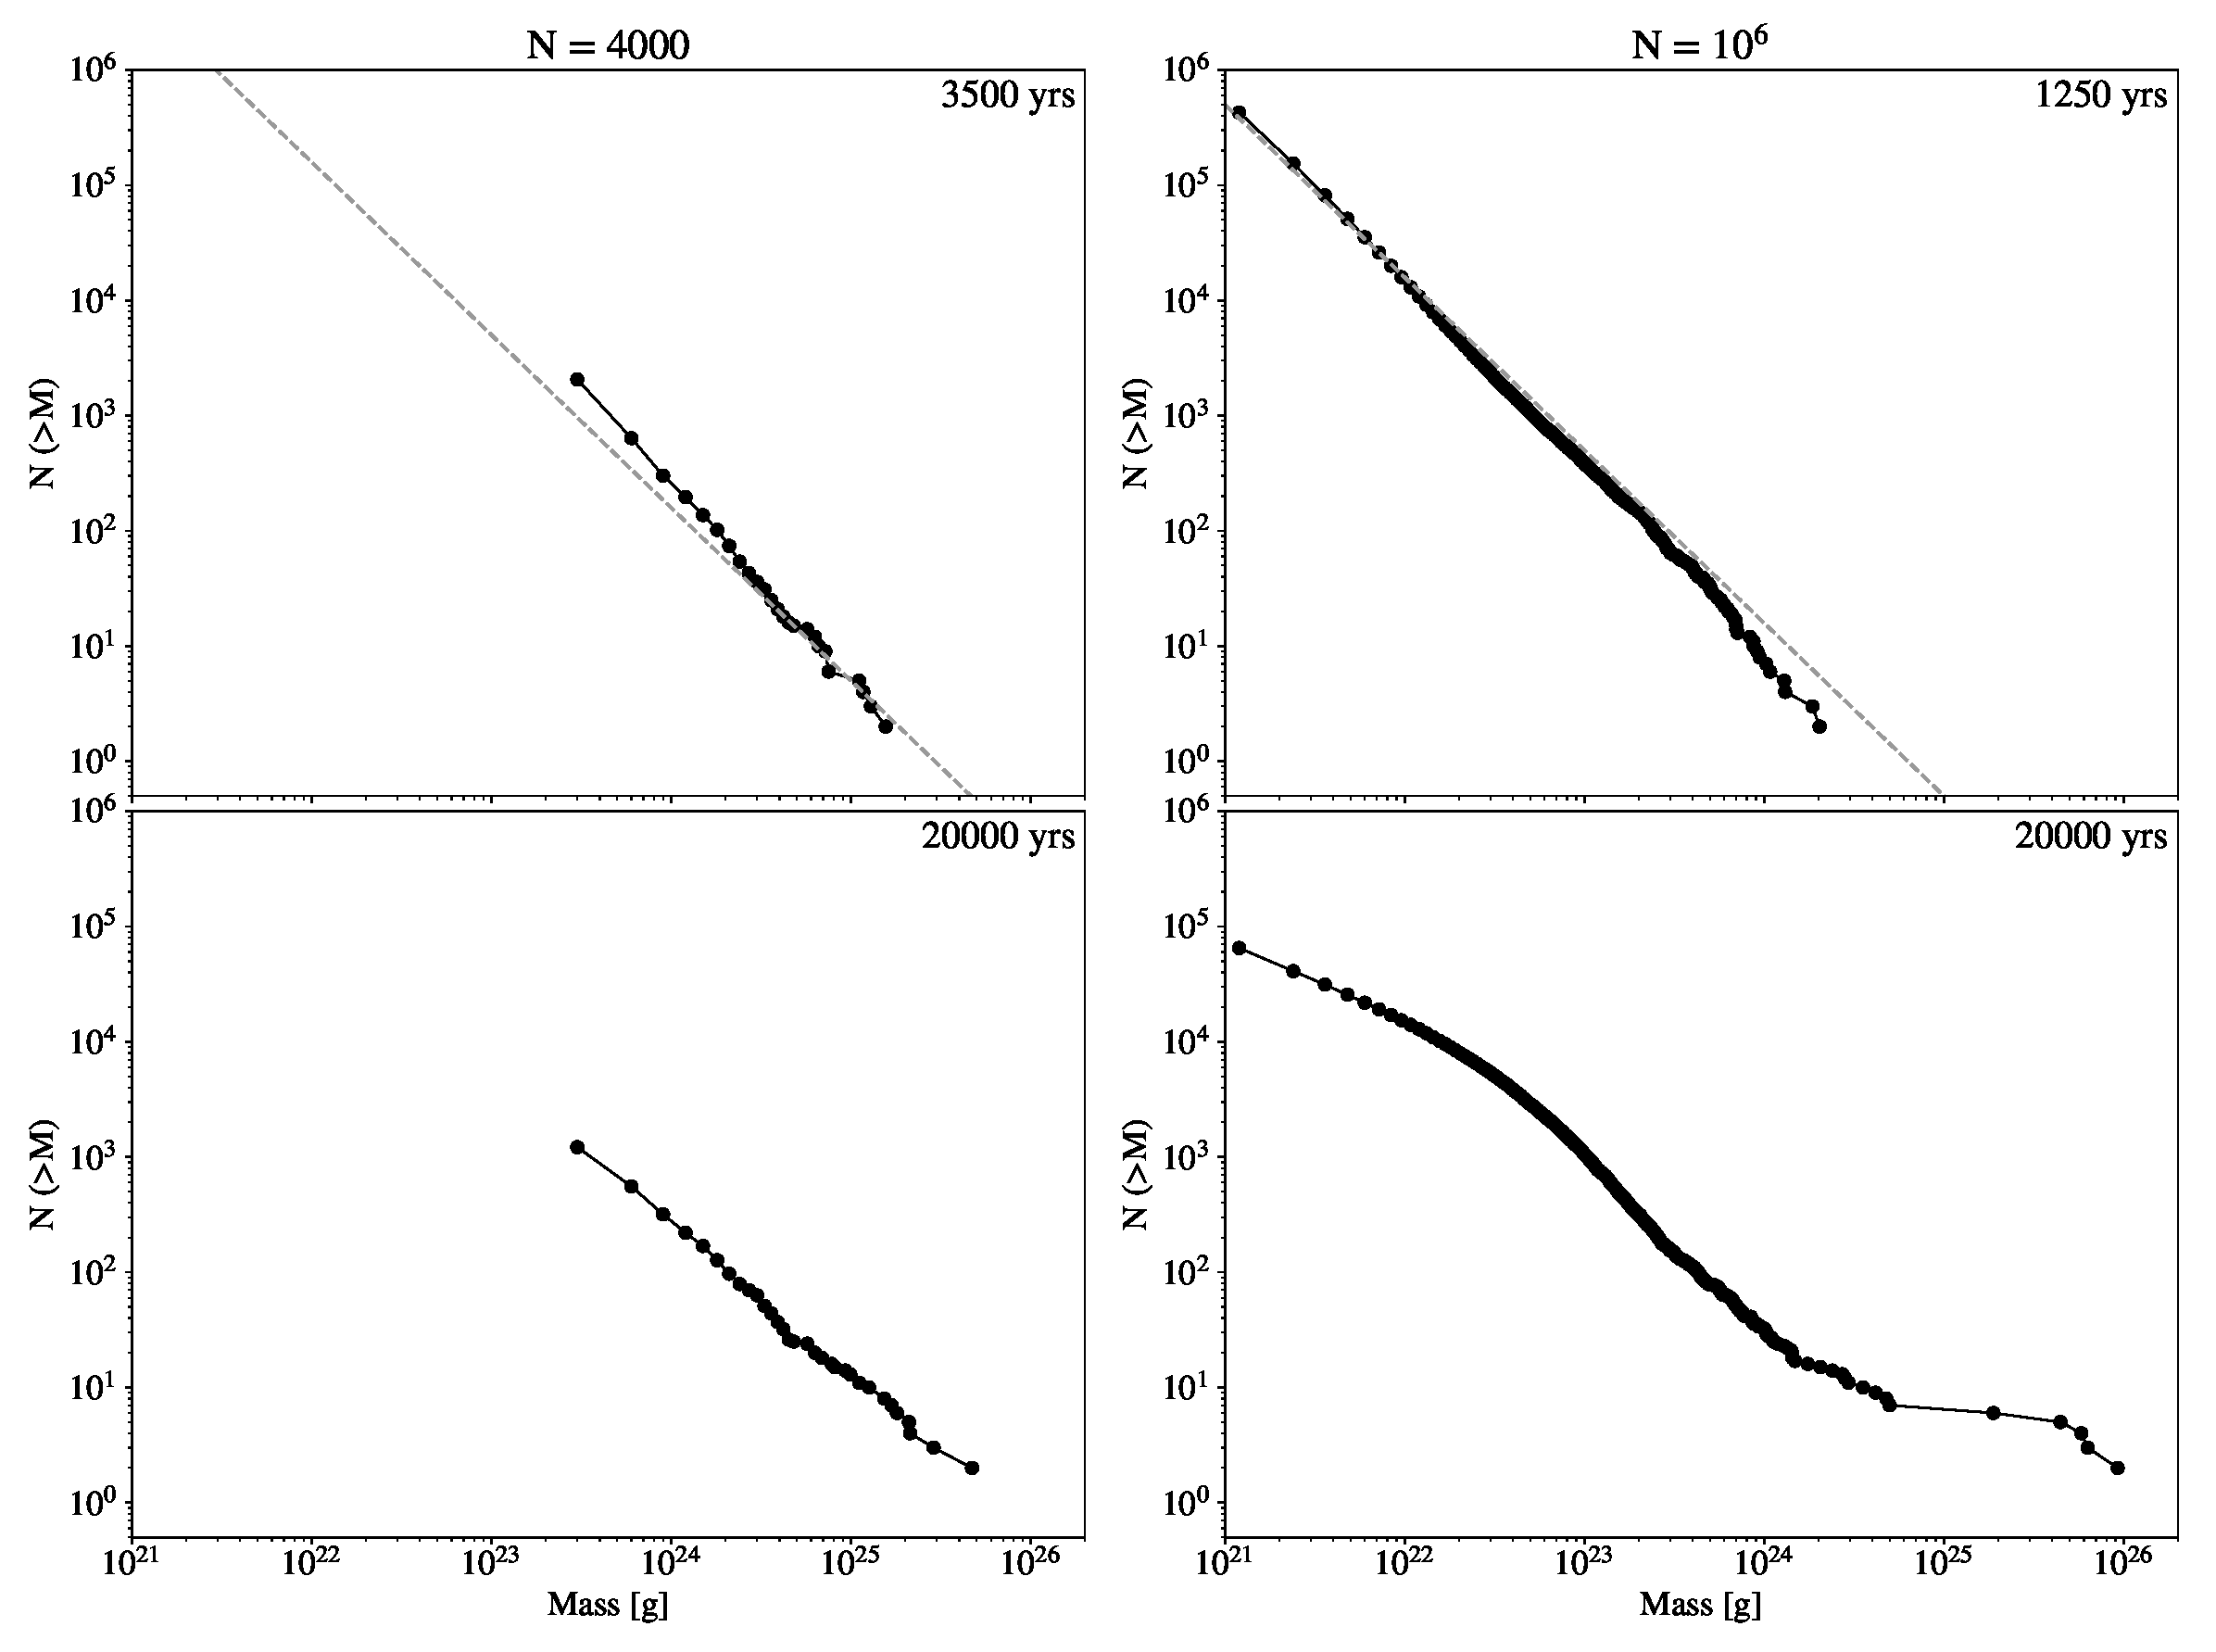
\includegraphics[width=\textwidth]{figures/plSS/mass_spectrum_evo.eps}
    \caption{Cumulative number of bodies in each mass bin for the low and high resolution runs, shown at the end of runaway growth (top row) and the end of the simulation (bottom row). The dashed line indicates a slope of -1.5, which is characteristic of runaway growth.
    \label{fig:mass_spectrum_evo}}
\end{figure}

% TODO: Is this described by the schmochwski equation (citation)?

\section{Results} \label{sec:plSS_results}

\subsection{Low vs High Resolution}\label{sec:lowvshigh}

We begin by comparing the evolution of growth between the low resolution (N=4000) and high resolution (N=$10^{6}$) models. 
As planetesimals collide and grow, gravitational focusing becomes increasingly effective and the relative growth rate increases 
with mass \cite{greenberg78}. Figure \ref{fig:mass_evo} shows the evolution of the average and maximum planetesimal 
mass in both simulations. Runaway growth at early times is evident from the fact that the maximum mass grows more quickly 
than the mean mass. Eventually, the largest bodies begin to dynamically heat the neighboring planetesimals, which slows the 
growth rate of the largest bodies.

When gravitational focusing and dynamical friction are both effective, the growth rate of a planetesimal of mass $M$ is given by

\begin{equation}\label{eq:growth_rate}
\frac{dM}{dt} \propto \Sigma M^{4/3} e_{m}^{-2},
\end{equation}

\noindent where $\Sigma$ is the surface density of solid material and $e_m$ is the rms eccentricity of the planetesimals 
\cite{kokubo95}. Before the oligarchs form, the eccentricity dispersion is independent of mass and the fractional growth rate 
scales like $dM/dt \propto M^{4/3}$ \cite{wetherill93}. This implies that large bodies grow more quickly than small bodies, hence 
the runaway effect. Once the oligarchs form and dynamical friction becomes effective, energy equipartition causes the velocity 
dispersion to evolve toward $v_m \propto M^{-1/2}$\cite{ida93a}. Using $v_m \propto e_m$ \cite{lissauer93}, the growth rate 
during the oligarchic growth phase scales like  $dM/dt \propto M^{2/3}$. Note that this does not imply that smaller bodies grow 
more quickly than large bodies. Rather, the growth rates tend towards the same value. This is reflected in figure 
\ref{fig:mass_evo}, where the slope of the maximum mass curve flattens out to match the slope of the mean mass curve after a 
few thousand years.

Comparing the two panels in Figure \ref{fig:mass_evo}, it is also evident that the rate of growth is more vigorous in the high 
resolution case. This is due to the fact that the collision time-scale, given by 

\begin{equation}\label{eq:coll_timescale}
t_{coll} = \frac{1}{n \sigma v},
\end{equation}

\noindent is shorter in the latter case, where $n$ is the number density of planetesimals, $\sigma$ is the collision cross section 
and $v$ is the typical encounter velocity. The collision cross section depends on both the geometric cross section ($\propto 
N^{-2/3}$) and an extra term due to gravitational focusing ($\propto N^{-7/3}$), where $N$ is the total number of particles in the 
simulation and the total disk mass \textbf{and geometry} is fixed. Because the eccentricity and inclination dispersion (and therefore the scale height of 
the disk) are kept fixed between the low and high resolution simulations, the typical encounter velocity does not vary with $N$. 
Here, we retain only the leading order term for the collision cross section, in which case these quantities scale like $n \propto N$, 
$\sigma \propto N^{-2/3}$ and $v \propto const$ so that

\begin{equation}\label{eq:coll_timescale_N}
t_{coll} \propto N^{-1/3}.
\end{equation}

Figure \ref{fig:plSS_ae} shows the a-e distribution of planetesimals at three snapshots from both simulations. In both cases, the 
eccentricity dispersion grows as energy from Keplerian shear is transformed into random motion, an effect known as viscous 
stirring \cite{ohtsuki02}. The black circles denote the semi-major axis and eccentricity of the 6 largest bodies. The area of the 
circles indicates the mass of the bodies and the horizontal bars are each scaled to 5 times the Hill radius of the bodies. 
Gravitational scattering between the oligarchs, coupled with dynamical friction from the surrounding planetesimals, places the 
oligarchs on low eccentricity orbits that are spaced apart by a 5-10 Hill radii via orbital repulsion \cite{kokubo98}.

Next, we examine the evolution of the mass distribution of planetesimals. This is shown in Figure \ref{fig:mass_spectrum_evo}. At 
early times, both models exhibit a power law distribution $N(<M) \propto m^{-\gamma}$, where $\gamma$ = 1.5 for the small bodies. A mass 
distribution with this slope is characteristic of runaway growth \cite{wetherill93}. The top panels show the mass distribution from 
both simulations at the end of the the runaway growth phase. In all subsequent snapshots, the mass distribution deviates from a 
single power law as the most massive bodies break away from the distribution, signaling the start of oligarchic growth. This 
happens sooner in the high resolution case. The bottom panels show the mass distribution at the end of the simulation at T = 
20,000 years.

Besides the fact that growth is more vigorous at higher resolution, the final mass distribution of planetesimals in the $N = 10^{6}$ 
case develops a feature that does not appear in the low resolution model. In the low resolution case, the low mass end of the 
mass distribution of planetesimals retains a single power law slope. The high resolution model, on the other hand, develops a 
bump in the mass distribution near $10^{22}$ g.

\begin{figure}
    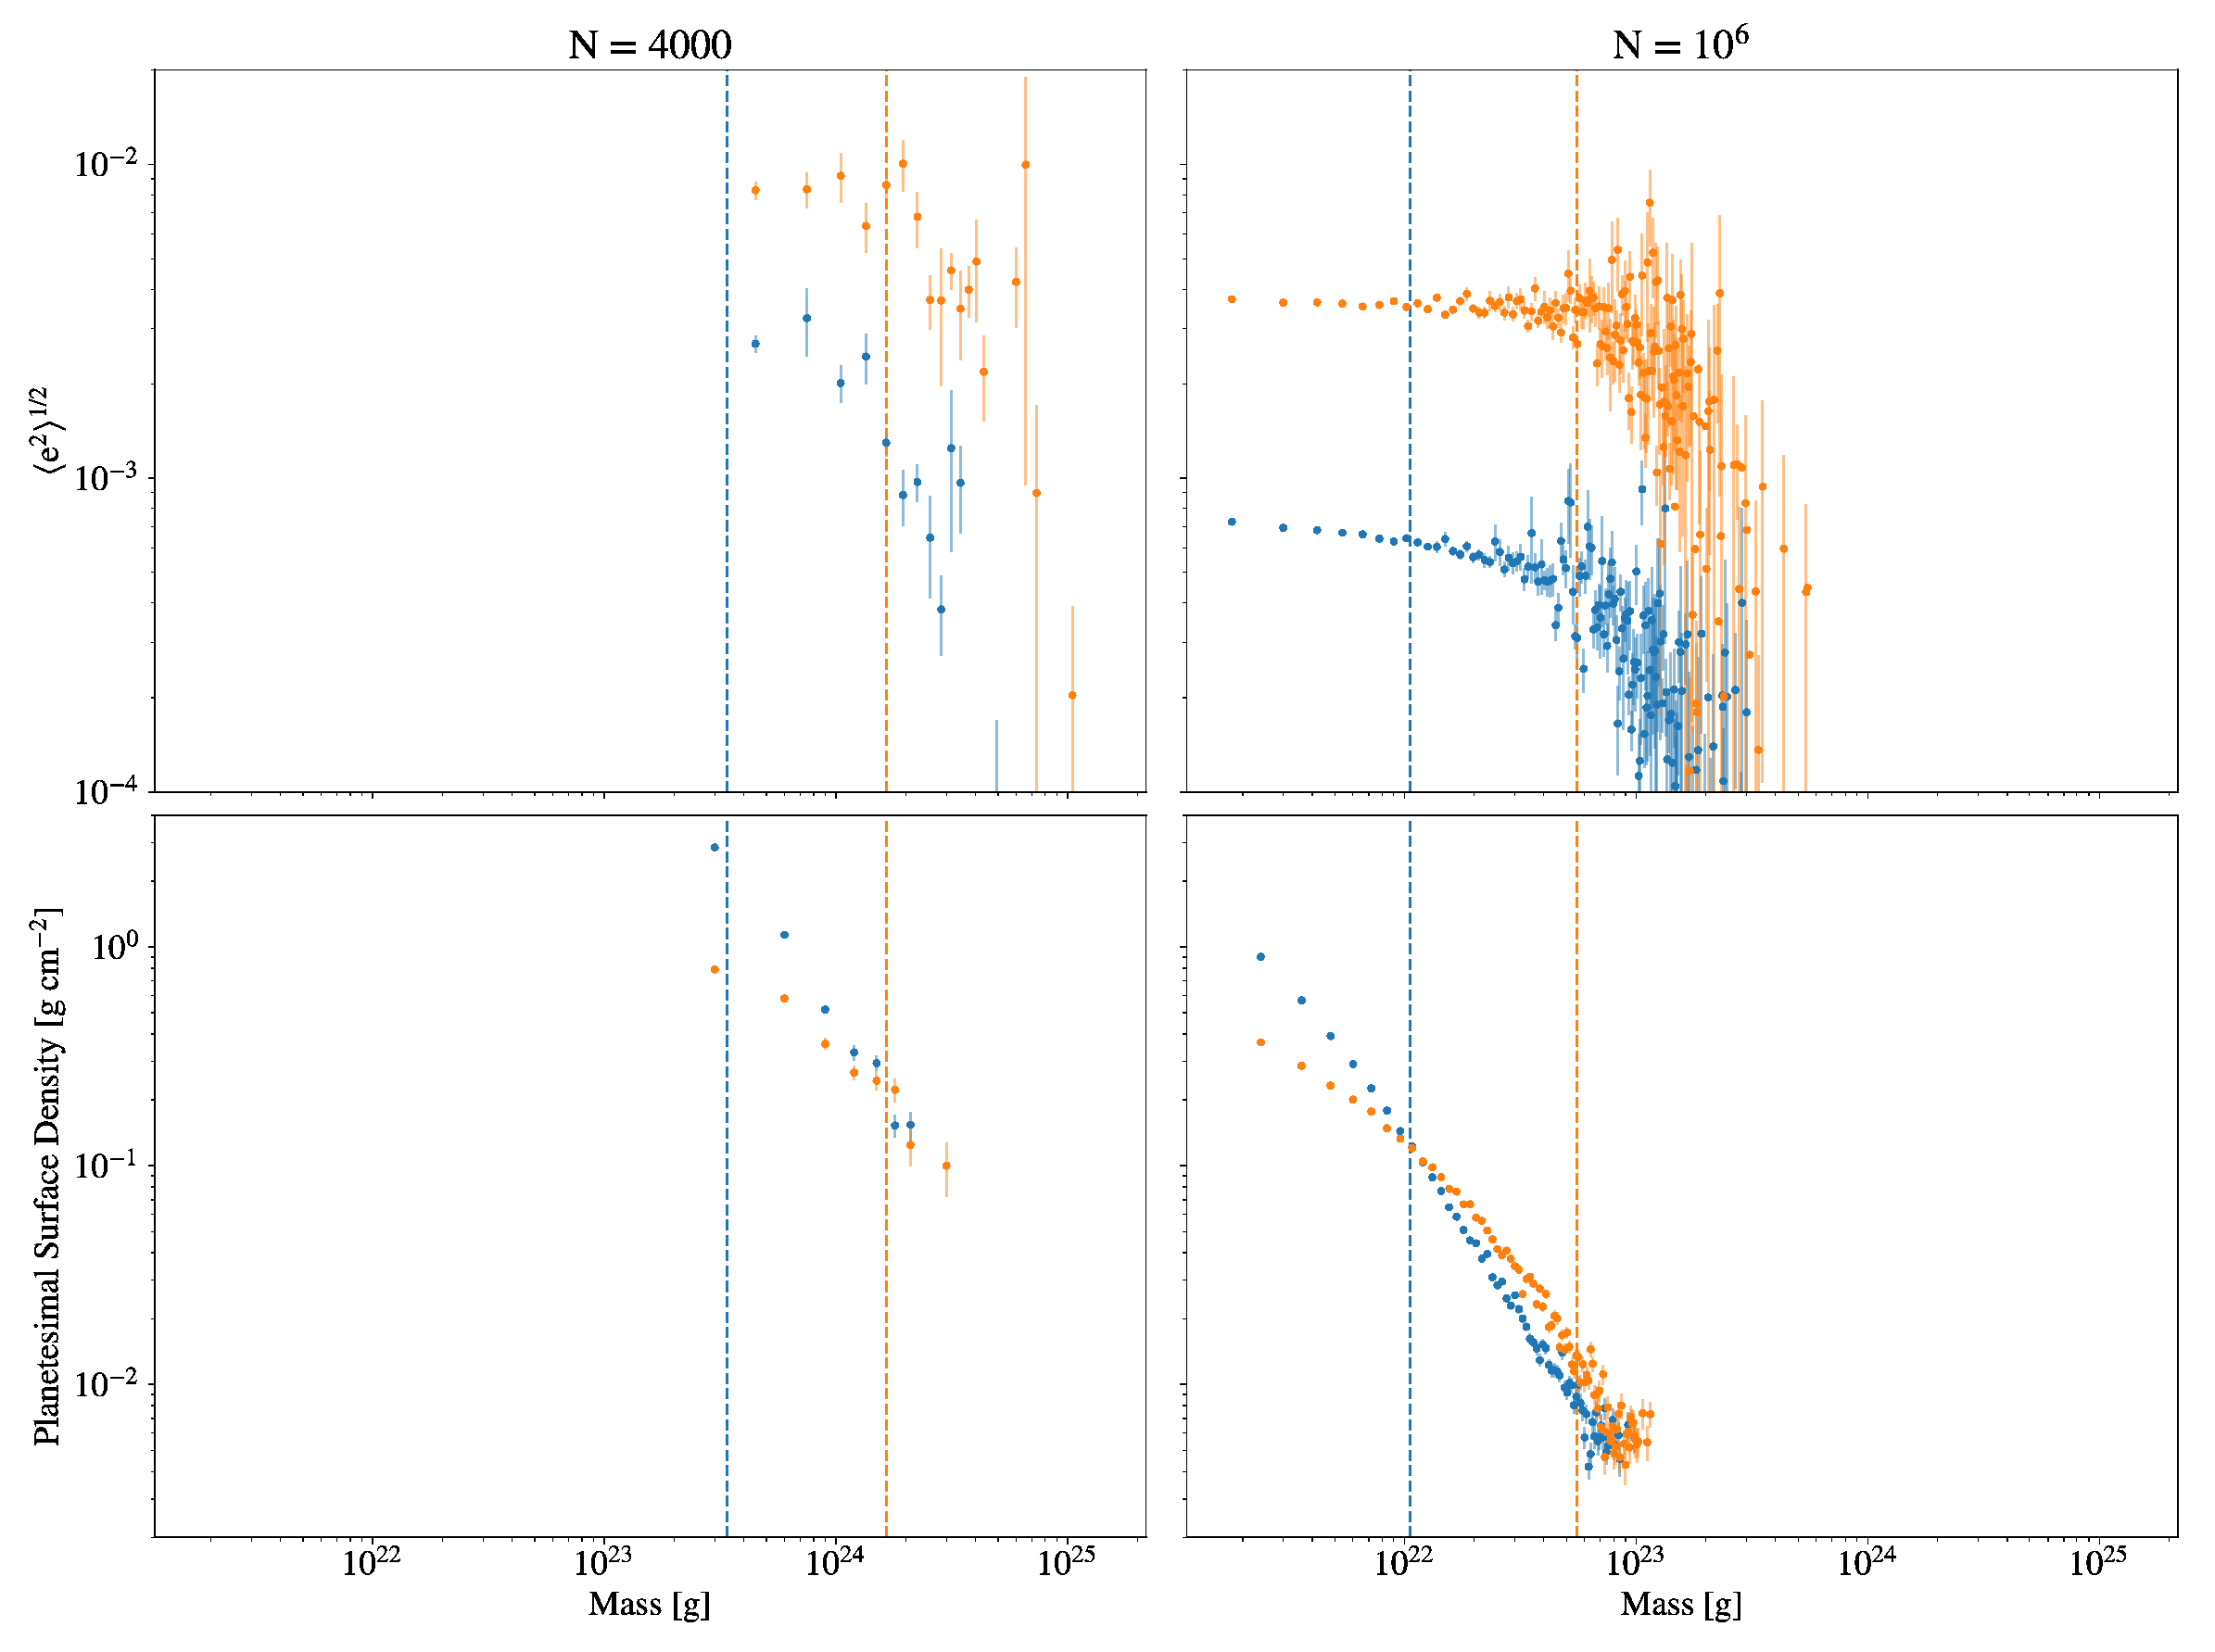
\includegraphics[width=\textwidth]{figures/plSS/ecc_den_evo.eps}
    \caption{The rms eccentricity (top) and planetesimal surface density at each mass (bottom) shown for the $N = 4000$ and 
    $N = 10^6$ simulations. The blue points correspond to the quantities at the end of the runaway growth phase (when the 
    mass distribution deviates from a single power law) and the orange points are from the end of the simulations (T = 20,000 
    years). The vertical dashed lines indicate the value of $M_{stir}$ \textbf{(defined by equation \ref{eq:mstir})} during that snapshot.}
    \label{fig:ecc_den_evo}
\end{figure}

\subsection{Explaining the Bump in the High Resolution Mass Spectrum}\label{sec:bump}

We would next like to determine what produces the feature at $10^{22}$ g in the high resolution simulation and why it is absent 
from the low resolution run. Upon close inspection of the simulation snapshots, both models retain a mass distribution that 
follows a single power law up until the onset of oligarchic growth. The bump in the high resolution mass spectrum becomes 
visible shortly after the oligarchs form. Over the course of the simulation, the bump gradually becomes more prominent. Because 
the bump appears shortly after the first oligarchs do, its presence is likely tied to the formation of the oligarchs.

Other investigations of planetesimal growth have revealed a similar bump in the size frequency distribution (SFD) at intermediate 
masses. \cite{morbidelli09} found that the location of this bump was set by the initial size of the planetesimals. Objects smaller 
than this size were created through disruptive collisions, which resulted in a shallower slope on the SFD to the left of the bump. 
Our collision model does not allow for fragmentation, so we must look for another explanation.

\cite{weidenschilling11} showed that a bump in the SFD was an artefact of the transition between shear and dispersion dominated 
growth. Objects in the shear regime, whose encounter velocities are dominated by the differential rotation of the disc, grow more 
slowly than those in the dispersion regime, whose encounters are set by the random velocity dispersion. Because the velocity 
dispersion varies with planetesimal mass, both of these growth modes can operate simultaneously. Energy equipartition should 
cause the velocity dispersion to decrease with mass, so the transition between shear and dispersion dominated growth should 
happen at some intermediate mass. Finally, the smallest bodies have a velocity dispersion that exceeds their escape velocities, 
which sets a third, slow mode of growth in which gravitational focusing is ineffective. Although our high resolution simulation 
resolves all three modes of growth, we find that the boundaries between these modes smoothly and steadily evolve. Over the 
course of the simulation, the shear-dispersion boundary increases from about $10^{22}$ g to $10^{25}$ g, while the \textbf{boundary at which the encounter velocity exceeds the mutual escape velocity} evolves from about $10^{21}$ to $10^{24}$ g. Any artifacts that these boundaries would leave on the 
planetesimal mass distribution should get washed out, so we also rule these out as explanations for the $10^{22}$ g bump.

Although the boundary between shear and dispersion dominated growth does not seem to be producing the bump, there still 
must be some kind of transition between growth modes occurring near this mass. As shown by equation \ref{eq:growth_rate}, 
the growth rate is controlled by both the surface density of the planetesimals and their eccentricities. In figure 
\ref{fig:ecc_den_evo}, we show the rms eccentricity and surface mass density of the planetesimals as a function of mass at the 
end of the runaway growth phase (blue points) and at the end of the simulation (orange points). In this figure, each point 
corresponds to the relevant quantity calculated for all planetesimals with the exact same mass. Because the simulations start 
with equal mass planetesimals which grow via pairwise collisions, the masses take on discrete, linearly spaced values. We found 
that logarithmically binning the mass values alters the shape of the distributions, especially in the high resolution case where the 
quantities span many orders of magnitude. For this reason, we chose not to bin any of the data. The error bars in figure 
\ref{fig:ecc_den_evo} are obtained via 10,000 iterations of bootstrap resampling. For the high resolution simulation, the error 
bars at low mass are smaller than the size of the points.

The surface density was determined by calculating an azimuthally averaged density profile using the analysis package
{\sc PYNBODY} \cite{pontzen13}. The surface density for each planetesimal mass was taken to be the average surface density 
for those particles in a single radial bin from 0.9575 to 1.0425 AU, which spans the initial boundaries of the annulus.

One might expect that the rms eccentricity spectrum should eventually reach energy equipartition ($e \propto m^{-1/2}$), but this 
has been shown to only occur with a sufficiently steep mass distribution \cite{rafikov03}. In our case, the mass distribution is 
shallow enough that the velocity evolution of the low mass bodies is set only by interactions with large planetesimals. The mass 
below which this occurs, shown by the vertical dashed lines in Figure \ref{fig:ecc_den_evo} is given by
\cite{wetherill93, ormel10}

\begin{equation}\label{eq:mstir}
M_{stir} = \frac{\left< m^2 \right>}{\left< m \right>}.
\end{equation}

Below this mass, planetesimals do not produce a dynamical friction wake and their velocity evolution becomes independent of 
mass \cite{rafikov03}. Because we started with equal mass planetesimals, the mass distribution was steep at early times. A 
power law slope steeper than $\gamma = 2$ should produce a mass-dependent velocity distribution everywhere \cite{rafikov03}. In 
the top right panel of Figure \ref{fig:ecc_den_evo}, the rms eccentricity distribution is not entirely flat below $M_{stir}$, which is 
likely due to the evolving mass spectrum. The analysis of \cite{rafikov03}, however, assumes a static mass spectrum.

At late times, a power law break in the surface density distribution forms near $10^{22}$ g in the high resolution simulation. 
Because the surface density is tied to both the mass distribution and the spatial distribution of planetesimals, it is difficult to learn 
anything else about the dynamics that are altering the growth rate from this information alone. We will examine this further in 
section \ref{sec:dynint}.

Given the power law break in the surface density distribution below $10^{22}$ g, we infer that there must be a dynamical 
mechanism at work that alters the collision rates of the low mass bodies. By the time that the $10^{22}$ g bump begins to 
appear, the planetesimals are sufficiently hot enough to render gravitational focusing ineffective (equation \ref{eq:growth_rate} is 
also no longer applicable). In this case, any additional heating actually increases the collision rate. In the next section, we examine how dynamical friction might be more effective with small planetesimals.

\section{Dynamical Friction and Resolution} \label{sec:dynfric}

Although the Chandrasekhar formula \cite{chandraesekhar43} contains no dependence on particle mass, the 'granularity' of the 
surrounding medium has been shown to influence the action of dynamical friction \cite{brunini07}. This is because the individual 
kicks from gravitational encounters become less frequent and more powerful at coarse resolution, introducing extra stochasticity 
as the system evolves toward energy equipartition. \cite{obrien06} showed that a finely resolved planetesimal distribution during 
the oligarchic growth phase produced planetary embryos with low eccentricities. They did not, however, examine the mass 
spectrum to see if the oligarchs were preferentially heating the smallest planetesimals. In addition, their simulations only 
contained a few thousand particles, while our high resolution run contains in excess of 200,000 bodies at the onset of oligarchic 
growth. Comparing the largest embryos at the end of simulation (i) to their results, we find that the largest embryo in our high 
resolution run has an eccentricity that is a factor of 2 smaller than the embryos produced by \cite{obrien06}.

In addition to altering the cumulative effect of close gravitational encounters, there is evidence that energy and angular 
momentum exchange through resonances is more effective with fine granularity. For example, in collisionless simulations of 
galaxies, \cite{weinberg07a, weinberg07b} showed that a minimum number of particles was required to populate 
resonances and couple the rotation of a bar to the central halo cusp through Lindblad resonances. If the resolution was too 
coarse, gravitational potential fluctuations would scatter particles out of resonances and prevent any strong torque between the 
bar and the halo. Likewise, \cite{cionco02} showed that resonant torque has a measurable effect on the interaction between a 
planet and a planetesimal disc.

\begin{figure}
    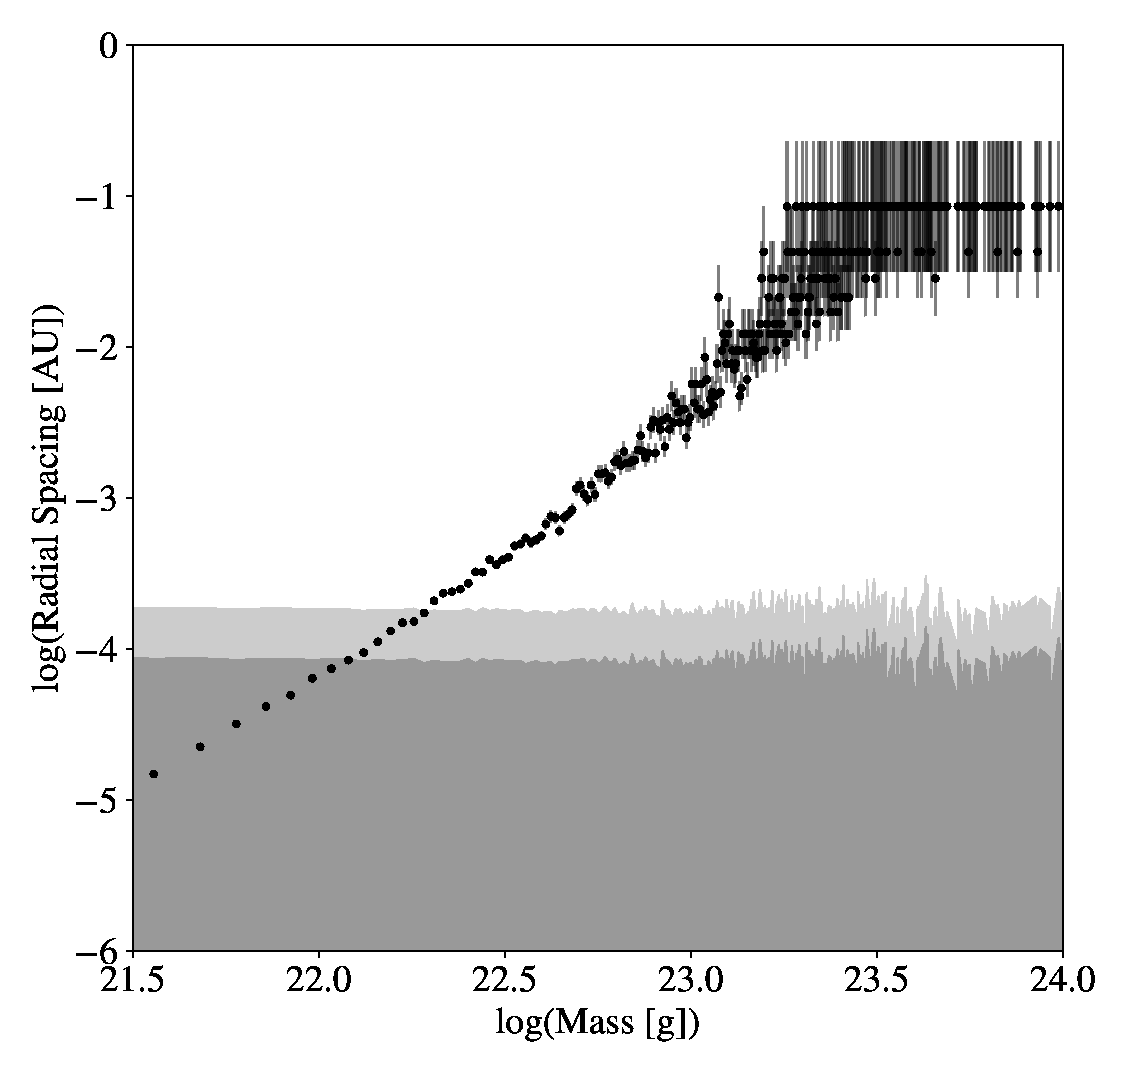
\includegraphics[width=\columnwidth]{figures/plSS/res_width.eps}
    \caption{The average spacing in semi-major axis as a function of mass at the end of the high resolution growth simulation 
    (black points). The gray regions indicate the libration width of planetesimals in each mass bin that are in resonance with the 
    most massive oligarch. The light gray region corresponds to the libration width of the 65:64 (highest non-overlapping) 
    resonance and the dark gray region corresponds to the 15:14 (most distant populated) resonance.}
    \label{fig:res_mass}
\end{figure}

% TODO: Why is this figure so large?

\subsection{Resolved Resonances}\label{sec:resonances}

During the oligarchic growth phase, a handful of massive bodies lose energy and angular momentum to the surrounding 
medium. The previous runaway growth phase leaves behind a steadily varying spectrum of planetesimal masses, whose number 
decreases with mass. Assuming the planetesimals are randomly distributed throughout the disc, the granularity can be thought 
of as increasing with mass. This implies that the dynamical friction should be more effective from the smallest planetesimals. 
Because the planetesimals appear to be more strongly heated below a certain mass threshold, we hypothesize that the change 
in growth modes has to do with the activation of resonances, rather than a smooth decrease in the stochasticity of scattering 
events.

Because spiral features like those seen in \cite{weinberg07a, weinberg07b} and \cite{cionco02} are unlikely to form in such a 
narrow annulus, we will consider the effects of mean motion resonances (MMRs), which are a subset of the Lindblad resonances 
considered in the aforementioned studies. In order to determine the resolution required to resolve MMRs, we calculate the 
libration width of first order MMRs associated with the oligarchs and compare it to the average radial spacing between 
planetesimals as a function mass. The average radial spacing is given by

\begin{equation}\label{eq:spacing}
\left< \Delta r \right> = \frac{\Delta a}{N(m)},
\end{equation}

\noindent where $\Delta a$ is the width of the annulus and $N(m)$ is the number of planetesimals of each mass.

Because the mass distribution has a negative slope and we expect planetesimals of varying mass to be randomly distributed 
about the disc, the radial spacing between planetesimals should increase with mass. For a fixed resonance width, there should 
be a cutoff in mass, below which planetesimals are more strongly affected by the resonances. The libration width of a first order 
mean motion resonance can be derived analytically using the pendulum approximation \cite{murray00} and is given by

\begin{equation}\label{eq:lib_width}
\frac{\delta a}{a} = \pm \left(\frac{16}{3} \frac{\left| C_{r} \right|}{n} e \right)^{1/2} \left(  1 + \frac{1}{27 j_{2}^2 e^3} \frac{\left| C_{r} \right|}{n} \right)^{1/2} - \frac{2}{9 j_{2} e}  \frac{\left| C_{r} \right|}{n},
\end{equation}

% TODO: Not applicable for small e, does this matter?

\noindent where $a$ is the semi-major axis at the center of the resonance, $e$ is the eccentricity of the body in resonance and 
$j_2 = -q$ where $p:q$ is the MMR being considered. $\left| C_{r} \right|/n = (m^{\prime}/m_{c}) \alpha f_{d}(\alpha)$, where $
(m^{\prime}/m_{c})$ is the mass ratio of the body associated with the resonance to the central body, $\alpha$ is the semi-major 
axis ratio associated with the resonance and $f_{d}(\alpha)$ is the disturbing function. For an interior first order resonance, the 
disturbing function can be expressed as

\begin{equation}\label{eq:dist}
f_{d}(\alpha) = j b_{1/2}^{j} + \frac{\alpha}{2}\frac{d b_{1/2}^{j}}{d \alpha},
\end{equation}

\noindent \cite{winter97} where $j = 1 - j_{2}$ and $b_{1/2}^{j}$ is a Laplace coefficient which is defined as

\begin{equation}\label{eq:lap}
b_{s}^{j}(\alpha) = \frac{1}{2 \pi} \int_{0}^{2 \pi} \frac{cos \, j \theta \, d \theta}{\left( 1 - 2 \alpha \, cos \theta + \alpha^2 \right)^{s}}.
\end{equation}

\noindent The derivative in the second term of equation \ref{eq:dist} can be written in terms of the Laplace coefficients 
\cite{murray00}

\begin{equation}\label{eq:lap_d}
\frac{d b_{s}^{j}}{d \alpha} = s \left( b_{s+1}^{j-1} - 2 \alpha b_{s+1}^{j} + b_{s+1}^{j+1} \right).
\end{equation}

Figure \ref{fig:res_mass} shows the libration width and average radial spacing of the planetesimals as a function of mass at the 
end of the high resolution run. To calculate the libration width as a function of planetesimal mass, the $e$ used in equation 
\ref{eq:lib_width} was taken to be the average eccentricity in each mass bin, while $a$ was set to the semi-major axis of the 
largest oligarch in the simulation. The slight variation in the resonance width as a function of mass is due to the variation in 
eccentricity. The error bars on the radial spacing data are calculated from Poisson statistics.

This calculation was done for the 15:14 and 65:64 mean motion resonances. The 15:14 resonance is the most distant first order 
resonance relative to an oligarch at 1 AU that still lies within the annulus of planetesimals. The 65:64 resonance is the closest 
MMR for which the libration width is smaller than the spacing between resonances. Higher first order resonances should not 
exhibit any resolution dependence because they overlap. For planetesimals less massive than about $10^{22}$ g, the average 
particle spacing drops below the libration width. Bodies below this mass cutoff, which we will refer to as the resonance heating 
mass $M_{res}$, are more likely to populate MMRs. This provides an explanation for how the oligarchs are preferentially heating 
the low mass bodies. Comparing with Figure \ref{fig:ecc_den_evo}, the mass of the power law break in the surface density 
matches very closely with $M_{res}$, which also matches the location of the $10^{22}$ g bump in figure 
\ref{fig:mass_spectrum_evo}. Over the course of the simulation, $M_{res}$ increases by no more than a factor of 2, so the 
growth mode boundary could easily leave an imprint on the mass spectrum, unlike the shear/dispersion dominated growth 
boundary, which evolves from $10^{22}$ to $10^{25}$ g.

In the restricted three-body problem, the orbital parameters of a test particle receiving energy and angular momentum via a 
mean motion resonance will evolve such that

\begin{equation}\label{eq:tiss}
\frac{de}{da} = \frac{a^{3/2} - 1}{2 a^{5/2} e},
\end{equation}

\noindent where $a$ is in units relative to the semi-major axis of the perturbing body. In the above equation, the inclination is 
assumed to be negligibly small \cite{murray00}.

Equation \ref{eq:tiss} can be used to place an upper limit on the change in eccentricity that a planetesimal in resonance will 
experience. Because any $\delta a$ larger than the resonance width will remove the planetesimal from the resonant influence of 
the oligarch, $\delta e$ is also restricted by the resonance width. Taking $a \approx 0.95$ (the location of the 15:14 resonance), 
$e \approx 10^{-3}$ and $\delta a \approx 10^{-4}$ (the libration width of the 15:14 MMR) we predict a first order change in 
eccentricity of $10^{-4}$. This value is small relative to the rms eccentricity of the planetesimals, which explains why the effects 
of the  mean motion resonances are not visible in Figure \ref{fig:plSS_ae} or in the top right panel of Figure \ref{fig:ecc_den_evo}.

\begin{figure}
    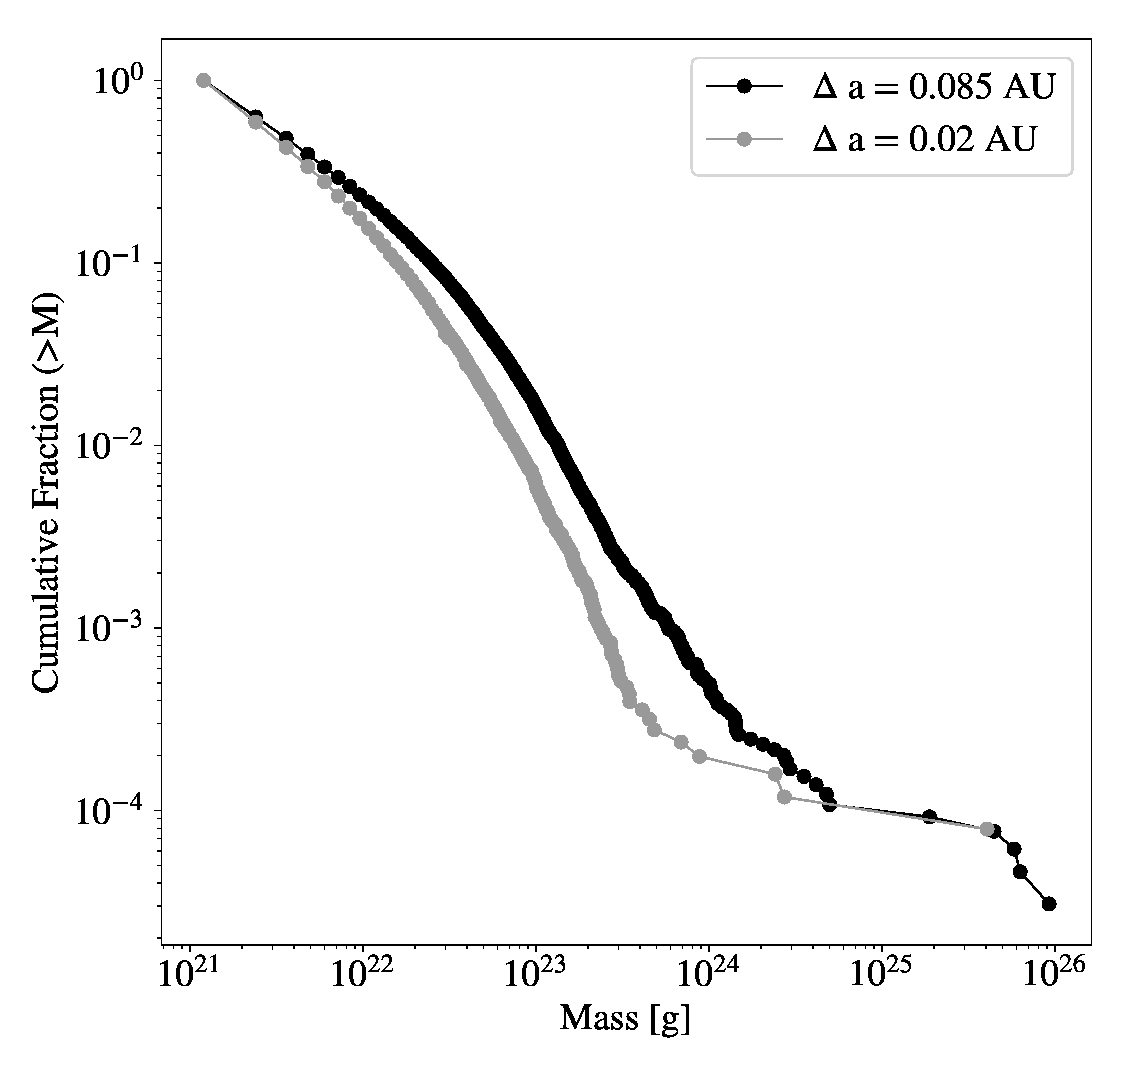
\includegraphics[width=\columnwidth]{figures/plSS/mass_spectrum_comp.eps}
    \caption{The cumulative fraction of bodies as a function of mass in the wide (solid dark curve) and narrow (gray curve) high 
    resolution growth simulations. Decreasing the annulus width, which depopulates resonances, produces a less prominent 
    $10^{22}$ g bump.
    \label{fig:mass_spectrum_comp}}
\end{figure}

% TODO: Large figure
% TODO: Bump isn't clear in this figure

Because the resonances are not possible to pick out by eye on an $a-e$ plot, we ran a modified version of simulation (i), the 
purpose of which is to show how planetesimal growth proceeds when the mean motion resonances are not present. The initial 
conditions are identical to those described in section \ref{sec:ics}, except that the annulus only extends from 0.98 to 1.02 AU. 
This effectively depopulates all of the first order mean motion resonances below the 26:25 resonance. It was not possible to use 
an annulus skinnier than this without introducing strong boundary effects which influence the growth of the planetesimals. This 
makes it impossible to depopulate all of the resolved resonances. The mass spectrum at the end of the skinny annulus 
simulation (also evolved for 20,000 years), along with the mass spectrum at the end of the high resolution growth simulation, is 
shown in Figure \ref{fig:mass_spectrum_comp}. With a narrower annulus, the change in slope of the mass distribution below 
$10^{22}$ g is noticeably weaker. We attribute this to the fact that the resonant interaction between the planetesimals and 
oligarchs is diminished because many of the MMRs are now empty.

\subsection{Planetesimal and Oligarch Mixing}\label{sec:mix}

Although figures \ref{fig:res_mass} and \ref{fig:mass_spectrum_comp} provide \textbf{circumstantial} evidence that the $10^{22}$ g bump is 
being produced by mean motion resonances, it is not immediately clear how the resonances affect such a large fraction of the 
planetesimals. To have a noticeable effect on the mass distribution, the oligarchs must be affecting bodies below $M_{res}$ 
everywhere in the disc, not just within the small fraction of space covered by the MMRs at a given time.

We infer that both the oligarchs and planetesimals slowly wander through the annulus due to occasional scattering events. This 
continually replenishes the population of planetesimals that are sitting inside of resonances. The orbital repulsion effect 
described by \cite{kokubo98}, which moves the oligarchs around, alters the location of the mean motion resonances. 
In addition, we infer that the planetesimals are occasionally scattered by the oligarchs. These two effects slowly cycle different 
planetesimals through the resonances and allow the oligarchs to eventually heat a large fraction of the small bodies.

\begin{figure}
    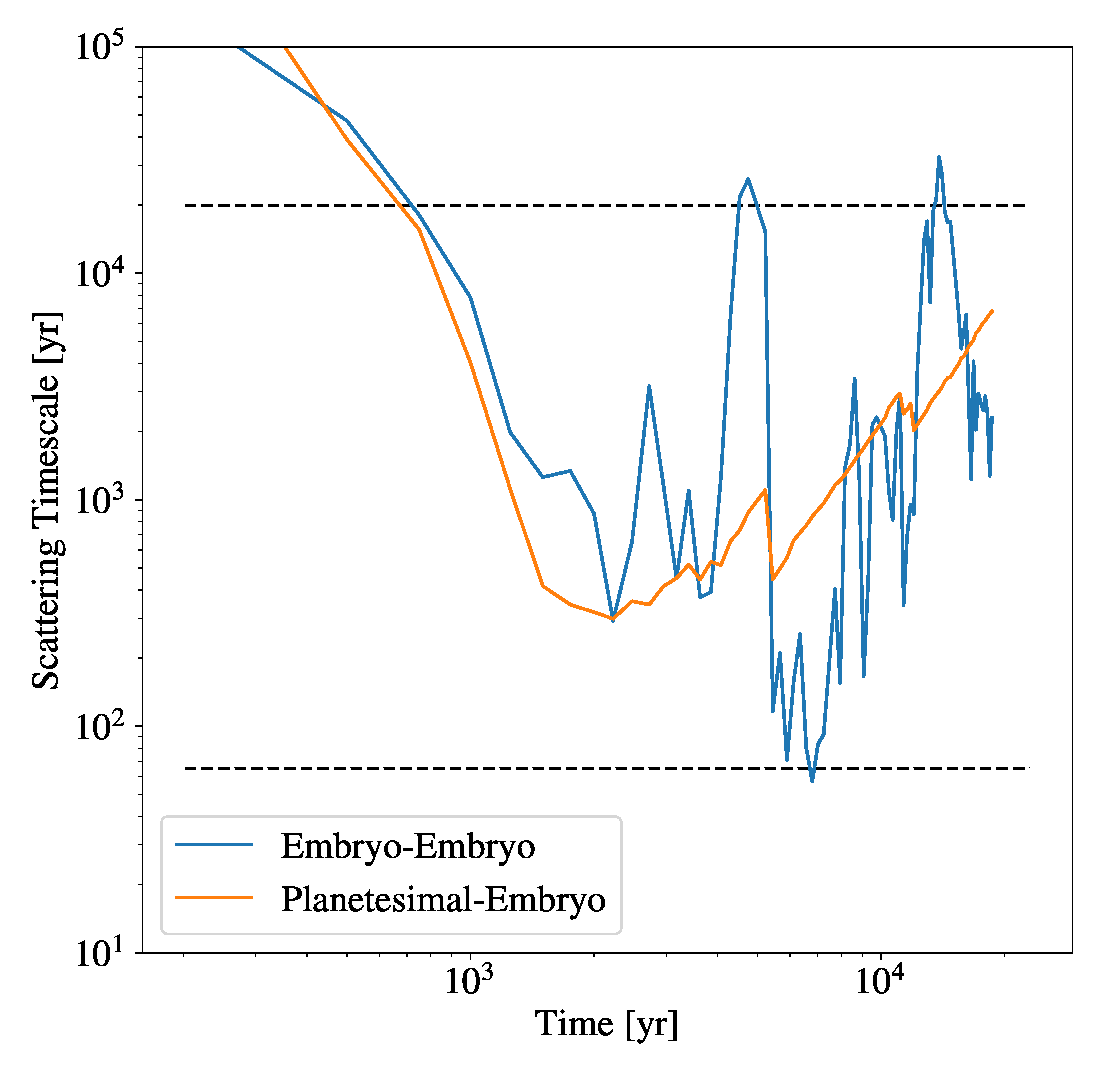
\includegraphics[width=\columnwidth]{figures/plSS/scatter_timescale.eps}
    \caption{The mean scattering time-scale for embryo-embryo (blue curve) and planetesimal-embryo (orange curve) interactions 
    over the course of the high resolution growth simulation. The dashed lines correspond to the simulation time-scale (upper) and 
    longest relevant mean motion resonance time-scale (lower), which is set by the 65:64 resonance.}
    \label{fig:scatter_timescale}
\end{figure}

% TODO: Large figure

In order for this effect to work, the bodies must keep a constant semi-major axis long enough for resonant interactions to play 
out, while still moving by an appreciable amount over the course of the simulation. The strong scattering time-scale for embryo-embryo interactions and planetesimal-embryo interactions is shown in Figure \ref{fig:scatter_timescale}. This is the timescale 
over which bodies of mass $m$ moving with speed $v$ relative to the local Keplerian velocity will approach each other with an 
impact parameter $b \leq G m / v^{2}$. This is sufficient to cause a large deflection and effectively randomize the orbital 
elements of the bodies. In both cases, the average time between scattering events falls between the longest resonance timescale (set by the 65:64 resonance) and the growth time-scale (set by the duration of the simulation). This indicates that the 
scattering is vigorous enough to occur many times over the course of the simulation, while still being slow enough to allow mean 
motion resonances to act. The strong scattering rate is given by

\begin{equation}\label{eq:scatter}
\dot{\overline{N}} \approx \frac{\Sigma}{m} \Omega_{p} R_{h}^2 \left( \frac{v_{h}}{v} \right)^{4},
\end{equation}

\noindent \cite{murrayclay06} where $\Sigma$ and $m$ are the surface density and individual masses of the bodies being 
scattered, $\Omega_{p}$ is the orbital angular velocity of the bodies and $R_{h}$ and $v_{h}$ are the Hill radius and Hill velocity 
of the object doing the scattering.

As discussed in section \ref{sec:lowvshigh}, viscous stirring plays an important role in the dynamical evolution of the 
planetesimals. The effects of viscous stirring are realized over many weak ($b \gg G m / v^{2}$) but frequent encounters. For a 
population of equal mass planetesimals, the timescale for viscous stirring is given by \cite{ida93}

\begin{equation}\label{eq:vs_timescale}
    \tau_{vs}  = \frac{\left< e^2 \right>}{d \left< e^2 \right> / dt} \approx \frac{1}{40}\left(\frac{\Omega^{2} a^{3}}{2 G m}\right)^{2} \frac{4 m \langle e^{2} \rangle^{2}}{\Sigma a^{2} \Omega},
\end{equation}

\noindent where $a$ and $e$ are the semi-major axes and eccentricities of the individual planetesimals. By using the properties 
of the planetesimal disk at the beginning of simulation (i) in equation \ref{eq:vs_timescale}, we find that the viscous stirring 
timescale is approximately 1000 years. This timescale can be taken as a lower limit because the eccentricity dispersion grows 
over time.

We also briefly consider the importance of planetesimal-driven migration. This is the coherent change in the semi-major axis of 
an oligarch due to repeated weak encounters with planetesimals. An upper limit on the planetesimal-driven migration rate of an 
oligarch is given by \cite{ida00}

\begin{equation}\label{eq:mig}
    \left| \frac{d a}{d t} \right| = \frac{a}{T} \frac{4 \pi \Sigma a^{2}}{M_{*}},
\end{equation}

\noindent where $a$ is the semi-major axis of the oligarch, $T$ is the orbital period of the oligarch and $\Sigma$ is the local 
surface density of the planetesimal disk. For an oligarch on a 1 AU orbit in a planetesimal disk with $\Sigma$ = 10 g cm$^{-2}$, 
the maximum migration rate is roughly $10^{-5}$ AU / yr. \cite{kirsh09} showed that this migration rate is greatly reduced for 
planetesimals whose encounters are dispersion dominated. In simulation (i), the Hill eccentricity of the smallest planetesimals at 
the onset of oligarchic growth is larger than 10, in which case the migration rate is reduced by a factor of at least 100 (see figure 
7 of \cite{kirsh09}). At this rate, it would take an oligarch roughly 1000 years to migrate by a single resonance width ($10^{-4}$ 
AU). This is much longer than the resonance timescale and therefore we do not expect that planetesimal-driven migration would 
disrupt the resonant configuration.

From these results, we conclude that the two simultaneous modes of growth are driven by a difference in the way that loosely 
and densely packed populations of planetesimals exert dynamical friction on large bodies. In the tightly packed case, energy 
transfer between the oligarchs and planetesimals is facilitated by mean motion resonances with the largest bodies.

\begin{figure*}
    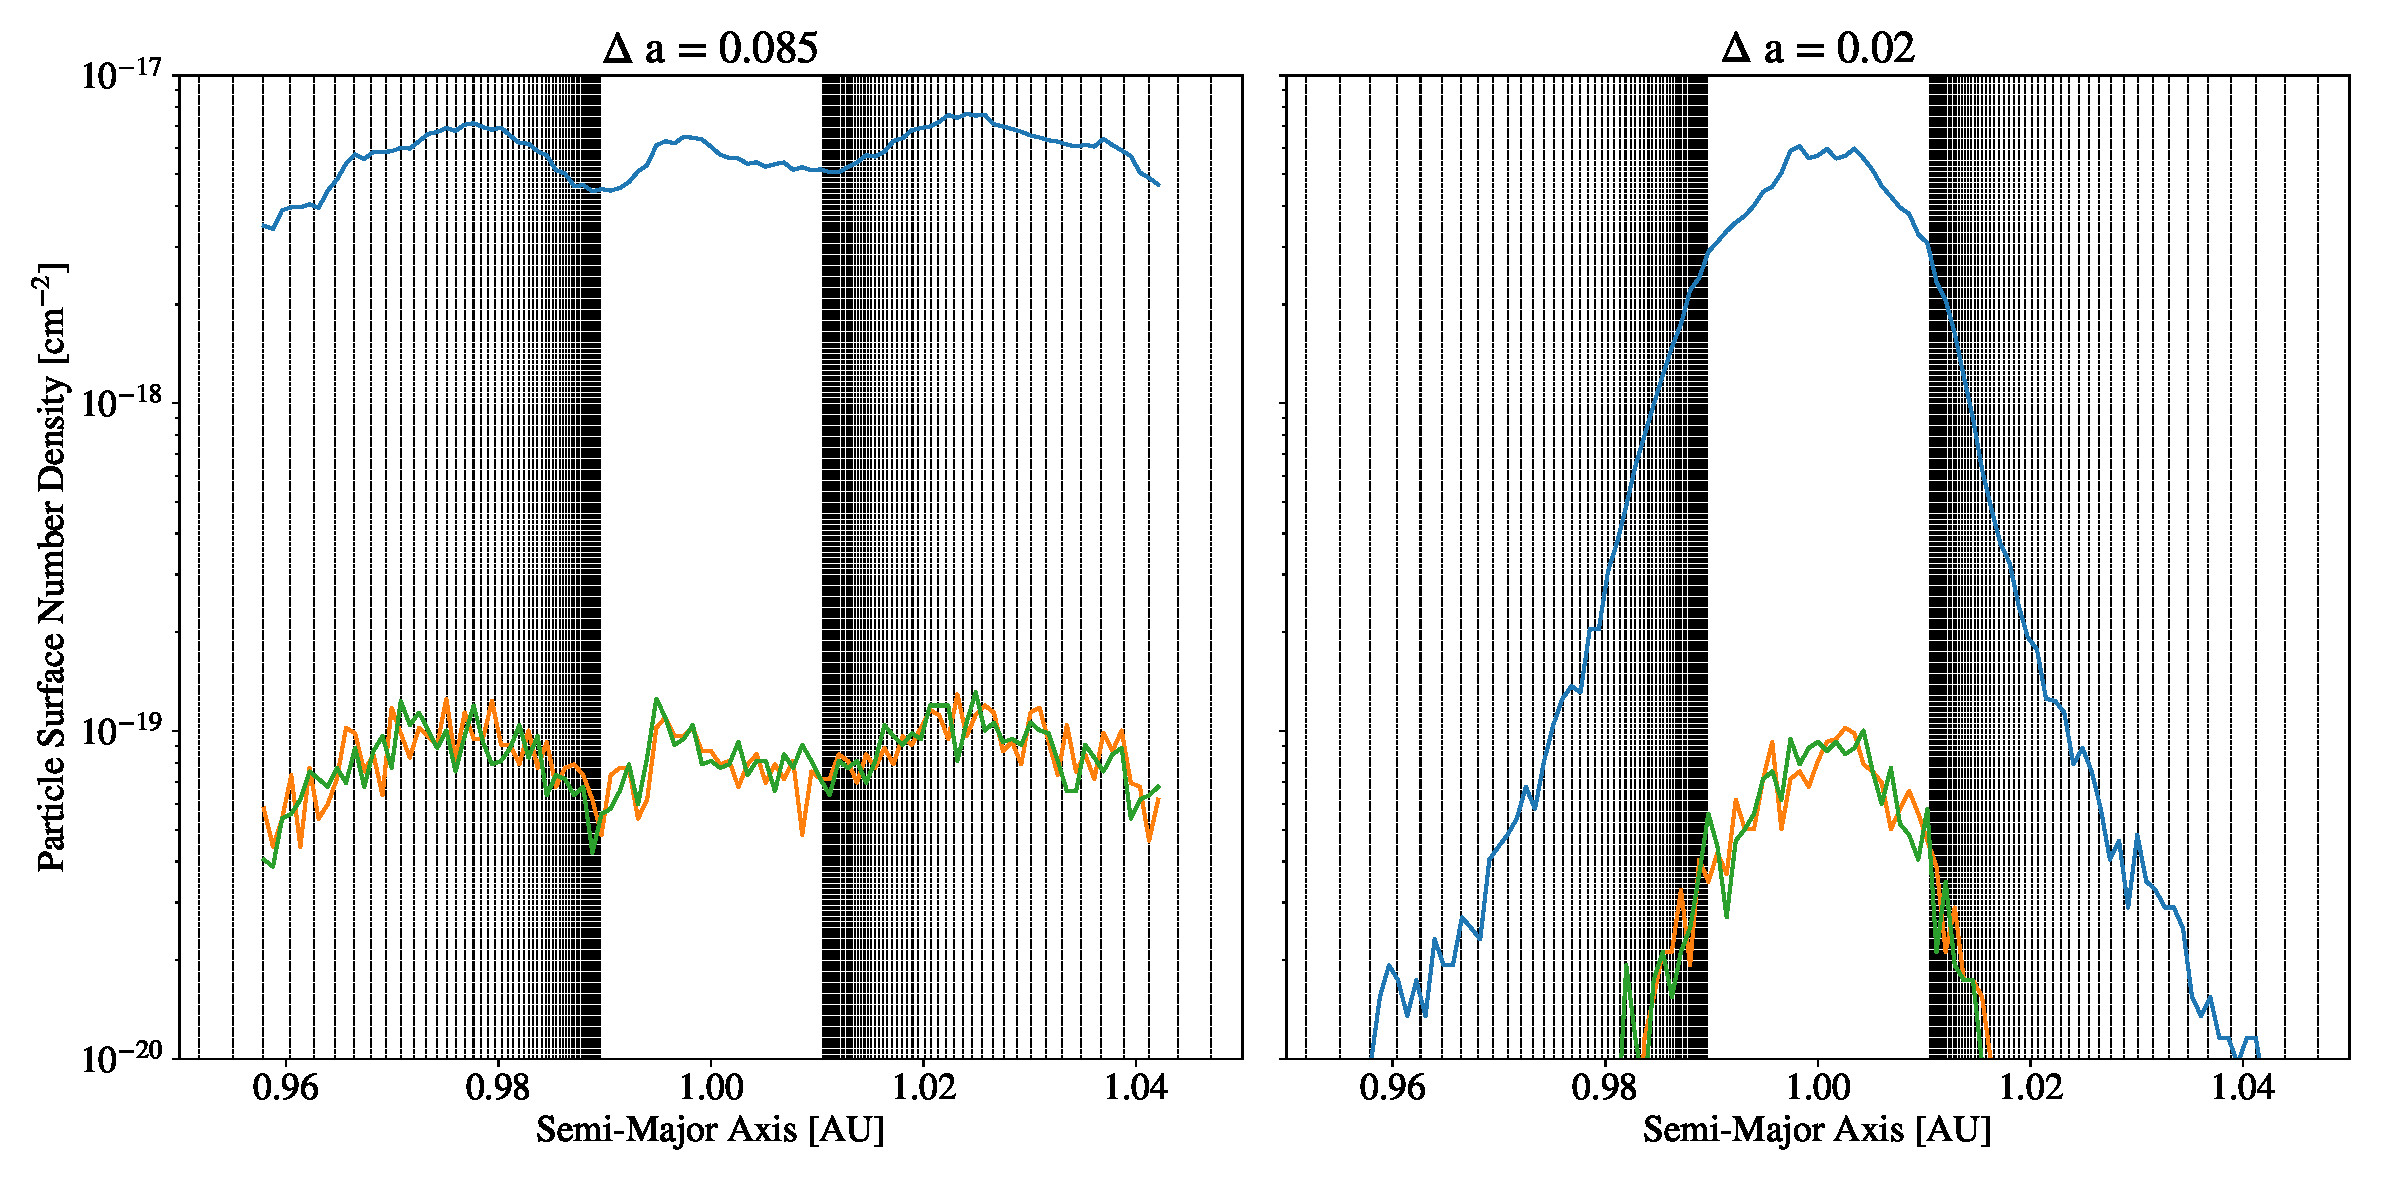
\includegraphics[width=1.0\textwidth]{figures/plSS/surf_den_dyn_fric.eps}
    \caption{Number density profiles of the planetesimals at the end of the $e_{hi}$ (left) and $e_{narrow}$ simulations (right). 
    The blue curves represent the number density of planetesimals less massive than the resonance heating mass ($2 \times 
    10^{22}$ g) and the orange curves represent the number density of planetesimals above this mass. The green curves show 
    the surface number density of planetesimals randomly drawn from the low mass bin, such that the total number of bodies 
    matches that of the high mass bin. The vertical lines indicate the positions of first order mean motion resonances with an 
    embryo at 1 AU.}
    \label{fig:num_den}
\end{figure*}

\subsection{Collisionless Dynamics}\label{sec:dynint}

So far, the most compelling evidence of the resonance heating effect that we have shown is the power law break in the surface 
density distribution in the bottom right panel of Figure \ref{fig:ecc_den_evo}. Because the surface density depends on both the 
mass distribution and spatial distribution of the planetesimals, it is difficult to tell whether the power law break is caused by 
resonances moving the planetesimals around or is simply set by the mass distribution. To clear up this ambiguity, we ran an 
additional set of simulations in which a large planetary embryo is embedded in an annulus of planetesimals, this time ignoring 
the effects of collisions. This forces the mass distribution to be static.

% TODO: Make bump more clear in figure 2.4

The initial conditions for these simulations were taken from intermediate snapshots from the runs described in section 
\ref{sec:plSS_results}. Specifically, the initial conditions are taken from the end of the runaway growth phase, which correspond to the 
snapshots shown in the top row of Figure \ref{fig:mass_spectrum_evo}. Additionally, a planetary embryo is placed in the center of 
the annulus at 1 AU with an eccentricity of 0.02 and an inclination of 0.01. The mass of the embryo is set at $M = 10^{26}$ g, 
which is approximately the mass of the largest oligarch at the end of the high resolution simulation. Because collisions are 
ignored, \textbf{bodies are allowed to pass through each other and} close encounters are handled with a gravitational softening parameter, the length of which is set to \textbf{what would have been} the physical radius 
of the planetesimals. Both runs are integrated for 2,000 years with fixed timesteps of 0.0025 years. We will refer to the 
collisionless versions of these simulations as $e_{low}$ and $e_{hi}$, respectively. To further demonstrate that the dynamical 
excitation of the small planetesimals is driven by mean motion resonances, we also ran a high resolution collisionless simulation 
with planetesimals outside of the $a$ = 0.99 to 1.01 AU range excluded. We will refer to this simulation as $e_{narrow}$.

As we saw previously, the resonance heating effect manifests itself as an increase in the spacing of the low mass planetesimals. 
Figure \ref{fig:num_den} shows the planetesimal surface number density at the end of the $e_{hi}$ (left) and $e_{narrow}$ (right) 
simulations described above. The vertical dashed lines indicate the locations of the non-overlapping first order mean motion 
resonances with the embryo. The blue curves show the number density of planetesimals below the resonance heating mass, 
which is $2 \times 10^{22}$ g in this case. The orange curves show the number density of planetesimals above this mass. 
Finally, to demonstrate that the difference in dynamical behavior between the low and high mass planetesimals is a population 
effect, the green curve shows the number density of a subsample of planetesimals randomly drawn from the low mass group, 
such that the total number of planetesimals in the subsample matches that of the high mass group.

In both cases, the particle number density is slightly enhanced around 1 AU, which is due to bodies trapped in the corotation 
resonance with the embryo. For the wide annulus, the surface number density decreases and then begins to increase again 
approximately 0.01 AU away from the embryo. As is evident in the left panel of Figure \ref{fig:num_den}, the location at which the 
number density begins to increase corresponds to the location of the closest non-overlapping (j $<$ 65) mean motion 
resonances. Due to conservation of the Jacobi energy (see equation \ref{eq:tiss}), interior MMRs will push bodies inward, while 
exterior resonances move bodies outward. This effect was also observed by \cite{richardson00} (see model B) in that the 
density decreases to the right of interior resonances and increases to the left. Because our setup contains many closely spaced 
resonances, the cumulative effect is that the density smoothly increases as one moves through the resonances. 

Hence, the number density distribution acquires a `W' shape around the embryo, with the low points corresponding to the inner 
edges of the resonant regions. An inspection of the earlier snapshots from this simulation shows that the 'W' structure becomes 
deeper and narrower with time. This is consistent with our resonance heating argument because the resonance time-scale 
decreases as one moves away from the embryo. The stronger, closer resonances become effective last, causing the profile to 
deepen and narrow with time.

The strength of the resonance heating effect depends on the number density of bodies outside of the $0.99 < a < 1.01$ AU 
region, where the resonances are not overlapping. The `W' shaped structure relative to the noise of the high mass (orange) and 
subsampled population (green) is weak compared to the low mass population (blue) due to the fact that there simply aren't many 
bodies sitting within the resonances. This structure is entirely absent from the narrow annulus, shown in the right hand panel of 
Figure \ref{fig:num_den} because the planetesimal number density near the resonances is too low. We infer that this decrease in 
number density of the low mass bodies adjacent to the embryo must also be present in the high resolution growth simulation and 
is enhancing the collision rate below the resonance heating mass.

We also examine the eccentricity evolution of the planetary embryo in the three collisionless simulations, shown in figure 
\ref{fig:e_oli_evo}. A decrease in the eccentricity of the embryo indicates that energy is being lost to the planetesimals. A steeper 
drop in eccentricity implies that the exchange happens more quickly and that the effects of dynamical friction are stronger. Only 
when the resonances are properly resolved and populated does the exchange appear to happen quickly. In both the $e_{narrow}
$ and $e_{low}$ simulations, the decrease in eccentricity of the embryo is gradual. This implies that dynamical friction is stronger 
and energy and angular momentum exchange between the oligarchs and planetesimals proceeds faster when the mean motion 
resonance heating is effective. In the $e_{hi}$ simulation, the eccentricity of the embryo begins to drop more steeply after about 
1000 years. This effect is also noticeable for the $e_{narrow}$ simulation, although it happens sooner. Because we are suddenly 
dropping a massive body into the annulus of planetesimals, the system likely requires some time to return to a state of quasi-
equilibrium. The two-body relaxation time, which is well-described by the viscous stirring timescale \cite{ida93} appears to 
roughly coincide with the change in slope for each of the curves in Figure \ref{fig:e_oli_evo}, although the connection between the 
relaxation of the planetesimals and the eccentricity evolution of the oligarch is not immediately clear. In the $e_{low}$ simulation, 
the change in slope may not be visible due to the fact that the two-body relaxation time is nearly instantaneous due to the small particle count (the relaxation time scales as $N / \ln N$).

\begin{figure}
    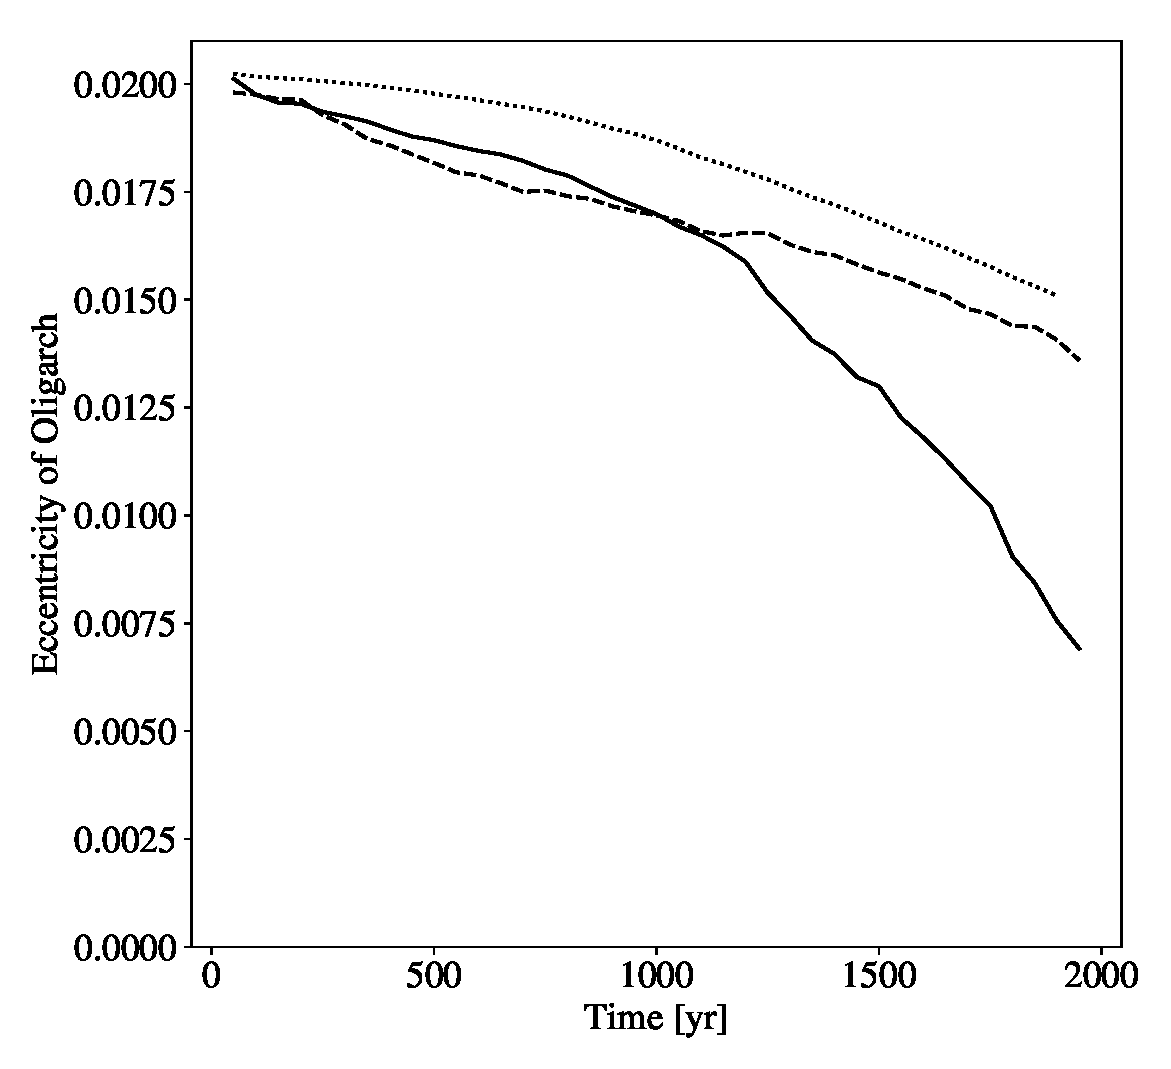
\includegraphics[width=\columnwidth]{figures/plSS/hetero_e_oli.eps}
    \caption{Time evolution of the eccentricity of the oligarch in the $e_{hi}$ (solid), $e_{narrow}$ (dotted) and $e_{low}$ (dashed) 
    simulation.}
    \label{fig:e_oli_evo}
\end{figure}

To verify the effectiveness of the resonant interactions, we next examine the evolution of the resonant arguments. The libration 
frequency of a planetesimal in resonance with an embryo is given by \cite{murray00}

\begin{equation}\label{eq:lib_period}
    \omega_{0}^{2} = -3 j_{2}^{2} C_{r} n e^{\left| j_{4} \right|},
\end{equation}

% TODO: wrong J coefficients here?

\noindent where $j_{2}$ = -15 and $j_{4}$ = -1 for the 15:14 MMR and $n = \sqrt{G M_{*} / a^{3}}$ is the mean motion of the 
planetesimal. For a planetesimal with a typical eccentricity of $10^{-3}$ inside the 15:14 mean motion resonance with a 
$10^{26}$ g embryo, the libration period is approximately 1000 years. For this reason, it is likely that a particle will undergo only 
a partial libration cycle before being removed from the resonance by two-body scattering. This makes it difficult to verify the 
resonant interaction by searching for libration, rather than circulation of the resonant arguments. However, this also implies that 
the resonances will cause permanent changes to the energy and angular momentum of the planetesimals. In canonical 
perturbation theory, the action conjugate to the resonant argument should evolve secularly because there is a near-constant 
term in the partial derivative of the Hamiltonian with respect to the resonant angle. If the viscous stirring timescale, which is the 
mechanism responsible for the removal of planetesimals from resonance is short compared to the libration period, this secular 
interaction produces a permanent change in the action (and therefore the energy and angular momentum) of a planetesimal 
(see the text following equation 10 in \cite{weinberg07a} for a further discussion of this).

The typical change in the resonant arguments of the planetesimals from the $e_{hi}$ simulation over multiple synodic periods is 
shown in Figure \ref{fig:lib_arg}. The resonant argument is given by \cite{murray00}

\begin{equation}\label{eq:res_arg}
    \phi = j_{1} \lambda_{e} + j_{2} \lambda_{p} + j_{4} \varpi_{p},
\end{equation} where $j_{1} = -j_{2} - j_{4} = 16$ for the 15:14 MMR. $\lambda_{e}$ and $\lambda_{p}$ are the mean longitudes 
of the embryo and planetesimal, respectively and $\varpi_{p}$ is the longitude of pericenter of the planetesimal. The $\Delta 
\phi$ shown in Figure \ref{fig:lib_arg} is the change in this resonant argument between t=1500 and t=1550 years, well after the 
system has relaxed back to a state of quasi-equilibirum. The blue diagonal lines represent the change in the resonant argument 
due to the Keplerian shearing of the disc. This quantity is derived by taking the time derivative of equation \ref{eq:res_arg},  
which is given by

\begin{equation}\label{eq:res_arg1}
    \frac{d \phi}{dt} = j_{1} \left( \frac{d \varpi_{e}}{dt} + \frac{d M_{e}}{dt} \right) + j_{2} \left( \frac{d \varpi_{p}}{dt} + \frac{d M_{p}}{dt} \right) + j_{4} \frac{d \varpi_{p}}{dt}.
\end{equation} Only the mean anomaly $M = n t$ changes due to the Keplerian shear and so

\begin{equation}
    \Delta \phi_{Kepler} = \sqrt{G M_{*}} \left( j_{1} a_{e}^{-3/2} + j_{2} a_{p}^{-3/2} \right) \Delta t,
\end{equation} where $\Delta t$ is the time interval that we are considering. Note that at the nominal resonance location, $\Delta \phi_{Kepler} = 0$.

\begin{figure}
    \includegraphics[width=\columnwidth]{figures/plSS/lib_arg.eps}
    \caption{The change in the resonant argument for the oligarch and planetesimals near the 15:14 MMR over a 50 year time 
    interval from the $e_{hi}$ simulation. The solid vertical line designates the nominal resonance location and the dashed vertical 
    lines indicate the minimum libration width. The diagonal blue lines represent the change in $\phi$ due to the Keplerian shear 
    of the disc, which is calculated analytically.}
    \label{fig:lib_arg}
\end{figure}

Over a 50 year time interval, which is approximately 3 times longer than the synodic period with the embryo, the change in the 
resonant arguments of the planetesimals appear to be dominated by the differential rotation of the disc. Near the nominal 
resonance location, the change in $\phi$ is small. The fact that many planetesimals remain within the resonance width and 
undergo only small changes in $\phi$ over multiple synodic periods demonstrates that the resonant interaction between the 
planetesimals and the embryo is able to proceed. Because the libration period is not short compared to the scattering timescale, 
the resonant interactions will cause permanent changes to the energy and angular momentum of the planetesimals.

\section{Implications of Simplifying Assumptions}\label{sec:assumptions}

\subsection{Gas Drag}

Although the effects of gas drag are weak during the planetesimal accretion stage, we will briefly consider its effect to ensure 
that it would not alter or remove the $10^{22}$ g bump. One way to describe the importance of gas drag on a planetesimal is 
with the stopping time \cite{adachi76}. In the Stokes regime, where the mean free path of gas particles is much smaller than the 
radius of the planetesimals ($\lambda \ll$ s), the stopping time is given by

\begin{equation}\label{eq:t_stop}
    t_{s} = \frac{2 m}{C_{D} \pi s^{2} \rho_{g} v}.
\end{equation}

\noindent Here, $\rho_{g}$ is the local density of the gas and $C_{D}$ is the drag force coefficient, which is of order unity in this 
regime. The gas density of the solar nebula is approximately $2 \times 10^{-9}$ g cm$^{-3}$ at 1 AU \cite{hayashi81}.

The relative velocity between the planetesimals and the gas is set by both the random motions of the planetesimals and the fact 
that the gas orbits at a sub-Keplerian speed due to its internal pressure support. The planetesimal velocity due to random 
motions is given by \cite{lissauer93}

\begin{equation}\label{eq:vrnd}
    v_{rnd} = v_{k} \sqrt{\left< e^2\right> + \left< i^2\right>}.
\end{equation}

\noindent At the beginning of the simulation (i), $v_{rnd}$ is on the order of $10^3$ cm s$^{-1}$. The headwind speed due to the 
sub-Keplerian motion of the gas is given by \cite{adachi76}

\begin{equation}\label{eq:vgas}
    v_{gas} = v_{k} \left( 1 - (1 - 2 \eta)^{1/2} \right),
\end{equation}

\noindent \textbf{where $\eta$ is a dimensionless parameter that describes the strength of the headwind.} At 1 AU in the solar nebula, $\eta \approx$ 0.002, which gives $v_{gas} \approx$ 6000 cm s$^{-1}$. From equation 
\ref{eq:t_stop}, the smallest planetesimals in simulation (i) have a stopping time on the order of $10^4$ years. This is much 
longer than the synodic period of the relevant planetesimal-oligarch resonances, therefore we expect the dynamics of even the 
smallest planetesimals to be entirely dominated by the resonances.

Additionally, gas drag can drive the inward radial drift of small bodies. Although the relatively large stopping time of the 
planetesimals suggests that this effect should be unimportant, the resonances are narrow enough that even a small amount of 
radial drift could quickly remove planetesimals from their influence. The radial drift velocity of a particle is given by 
\cite{weidenschilling77}

\begin{equation}\label{eq:v_drift}
    v_{r}  = -\frac{2 v_{gas}}{\Omega t_{s} + \left( \Omega t_{s} \right)^{-1}}.
\end{equation}

\noindent where $\Omega$ is the orbital angular frequency of the body being considered. Using the values for $v_{gas}$ and 
$t_{s}$ described above, the inward radial drift speed of the smallest planetesimals is 0.1 cm s$^{-1}$. At this rate, a 
planetesimal will drift across a typical resonance width ($10^{-4}$ AU) in about 1000 years. This is comparable to the viscous 
stirring timescale, which suggests that radial drift should not have a significant effect on the resonant dynamics.

Massive bodies can create density waves in the gas disk which carry away angular momentum \cite{goldreich79, goldreich80} 
through an effect known as type I migration (for a recent review see \cite{baruteau14}). The strength of this effect scales linearly 
with the mass of the body and should therefore be most effective for planetary embryos. In addition to gas drag causing 
planetesimals to radially drift across resonances, type I migration can cause planetary embryos to drift inwards, potentially 
moving the resonances before they have a chance to act on the planetesimals. \cite{tanaka02} provides an analytic expression 
for the torque exerted on a body embedded in a three-dimensional gaseous isothermal disk as

\begin{equation}\label{eq:t1mig_torque}
     \Gamma = -\left( 1.364 + 0.541 \alpha \right) \left (\frac{m}{M_{*}} \right)^{2} \left( \frac{r \Omega}{c_{s}} \right)^{2} \Sigma r^{4} \Omega^{2},
\end{equation}

\noindent where $\alpha$ is the power law index of the radial surface mass density profile $\Sigma \propto r^{-\alpha}$ of the gas 
and $c_{s}$ is the local sound speed of the gas, $m$ is the mass of the body, $\Omega$ is the orbital angular frequency of the 
body and $r$ is the orbital distance of the body. The radial migration velocity is given by

\begin{equation}\label{eq:t1mig_rate}
    \dot{r} = \frac{-2 r \Gamma}{L},
\end{equation}

% TODO: Ask rory about concern that alpha = 3/2 too large?

\noindent where $L = m \left( G M_{*} r \right)^{1/2}$ is the total angular momentum of the body. For a $10^{26}$ g embryo 
orbiting at 1 AU and taking $\alpha$ = 3/2, $\Sigma$ = 1700 g cm$^{-2}$ and $c_{s}$ = $10^{5}$ cm s$^{-1}$ \cite{hayashi81}, 
the inward migration speed is $2 \times 10^{-7}$ AU yr$^{-1}$. At this rate, the 15:14 MMR with an embryo will migrate by a 
entire resonance width in roughly 500 years, which is much longer than the synodic period. It should be noted that the analysis 
of \cite{tanaka02} has been shown to produce migration rates that are up to a factor of $10^{3}$ too large to be consistent with 
observed populations of exoplanets \cite{ida04, alibert05, miguel11}. The migration timescale derived above should therefore 
be taken strictly as a lower limit.

As migration proceeds, planetesimals can have their spatial distribution altered as they become trapped in exterior resonances 
with protoplanets \cite{weidenschilling85}. A necessary condition for resonant trapping to occur is that the drift timescale of a 
planetesimal across a resonance must be much longer than the libration period \cite{dermott88}. As we calculated in section 
\ref{sec:dynint}, a typical libration period is around 1000 years. This is comparable to the timescale for \textbf{two-body} 
scattering and also for radial drift of planetesimals across a resonance due to gas drag. Therefore, we do not expect that exterior 
resonances should be effective at trapping drifting planetesimals.

\subsection{Inflated Collision Cross Section}

As discussed in section \ref{sec:collModel}, enhancing the geometric collision cross section $f$ of the planetesimals by a factor 
of 6 only slightly reduces the effectiveness of gravitational scattering. More importantly, varying $f$ alters the accretion 
timescale. The implication of this is that a longer accretion timescale causes oligarchic growth to commence later when the disk 
is more dynamically excited. The dynamical excitation of the disk, which is set by the rms eccentricity, alters the libration width of 
planetesimals in resonance with the oligarchs. In section \ref{sec:resonances}, we argued that the intersection between the 
libration width and the radial spacing between planetesimals sets the location of the bump in the mass distribution. Because the 
radial spacing between planetesimals increases with mass and the libration width of the resonances gets larger with time, the 
mass of the bump would be larger had we used $f$ = 1.

It is difficult to predict exactly how much $f$ reduces the accretion timescale, but \cite{kokubo96} showed that it is by no more 
than factor of $f^2$. Integrating equation \ref{eq:vs_timescale}, the rms eccentricity scales with $t^{1/4}$. Having enhanced the 
collision cross section by a factor of 6, the rms eccentricity should be a factor of $(f^2)^{1/4} \approx 2.5$ times larger with a 
realistic collision cross section. Using equation \ref{eq:lib_width}, a factor of 2.5 increase in the eccentricity of a planetesimal 
increases the libration width by a factor of about 1.6. Looking at Figure \ref{fig:res_mass}, this would cause an extremely 
insignificant \footnote{The difference in libration width between the 65:64 and 15:14 resonance produces a much larger spread in the exact value of the resonance heating mass.} change in the resonance heating mass.

\subsection{Fragmentation}

Because our model does not include the effects of collisional fragmentation, we examine the statistics of the collisions in 
simulation (i) to estimate its effects had it been included. Here, we find that roughly 60 percent of the collisions occur with a 
relative velocity larger than the mutual escape velocity of the two planetesimals. Assuming that the planetesimals are rubble 
piles with no internal strength, these high velocity collisions should be completely disruptive. Previous studies of planetesimal 
accretion have shown that including the effects of fragmentation tends to slow down the accretion process, but does not 
qualitatively change it \cite{wetherill93, leinhardt05}.

If we separate the collision statistics into those occurring between bodies below the bump mass ($< 10^{22}$ g) and those 
above the bump mass, we do not see a significant difference in the relative amount of catastrophic collisions. Above the bump 
mass, about 60 percent of collisions occur at disruptive velocities, while 70 percent of collisions between bodies below the bump 
mass occur at these high relative velocities. Because we do not have multiple simulations to draw from, it is difficult to estimate 
errors to tell whether this difference is statistically significant.

Assuming that disruptive collisions are not significantly more common below the bump mass, we expect that fragmentation 
would alter our results by lengthening the accretion timescale. As discussed in the previous section, the location of the bump 
depends on the rms eccentricity of the planetesimals during the oligarchic growth phase. If this phase takes longer to 
commence, the libration widths of the resonances would be larger when the embryos form, which increases the mass below 
which the resonant heating is effective. Although it is difficult to determine by exactly how much fragmentation extends the 
accretion timescale, statistical models of planetesimal growth show that $10^{26}$ g embryos can be formed in $10^{5}$ years 
\cite{wetherill93} when the effects of fragmentation are included. We showed in the previous section that a factor of 36 increase 
in the accretion timescale (720,000 years) makes a negligible difference in the location of the bump in the mass spectrum. 
Similarly, we expect that including the effects of fragmentation would make a negligible contribution to the bump mass.

\section{Dependence on Initial Planetesimal Mass}\label{sec:intermed}

In order to demonstrate that our results are robust, and also to gain some insight into how the resonance heating mass is related 
to the initial planetesimal mass, we ran two more simulations of planetesimal growth at intermediate resolutions. Our choice of 
initial planetesimal mass in the high resolution simulation was somewhat arbitrary and understanding how this parameter affects 
the resulting distribution of masses is necessary in order to connect our results with observations of small Solar System bodies.

The configurations used were identical to the high resolution run described in section \ref{sec:ics}, except that the particle count 
was changed. These two additional runs contained 250,000 and 500,000 starting planetesimals, which corresponds to $m = 2.4 
\times 10^{21}$ and $m = 4.8 \times 10^{21}$ g, respectively, at the same surface density. To match the same eccentricity 
dispersion as the models described in section \ref{sec:ics}, we used $\langle e^2 \rangle^{1/2} = 3.17 h/a$ and $\langle e^2 
\rangle^{1/2} = 2.52 h/a$, with the inclination dispersion set to half of those values.

Figure \ref{fig:resolution_mass_dist} shows the mass spectrum at T = 20,000 years in the high resolution growth simulation, 
along with the intermediate resolution growth simulations mentioned above. In all three cases, the bump in the mass distribution 
approximately matches up with the resonance heating mass. There is a clear positive trend between the resonance heating 
mass and the initial planetesimal mass $m$, which we attribute to two things. First, larger planetesimals will be spaced further 
apart for a fixed disc surface density. This pushes the intersection point between the planetesimal spacing and libration width to 
higher mass. Secondly, larger initial planetesimals will cause oligarchic growth to begin at a higher mass \cite{morishima17}. 
This increases the libration width of the resonances, which moves the intersection between planetesimal spacing and resonance 
width to a higher mass.

\begin{figure}
    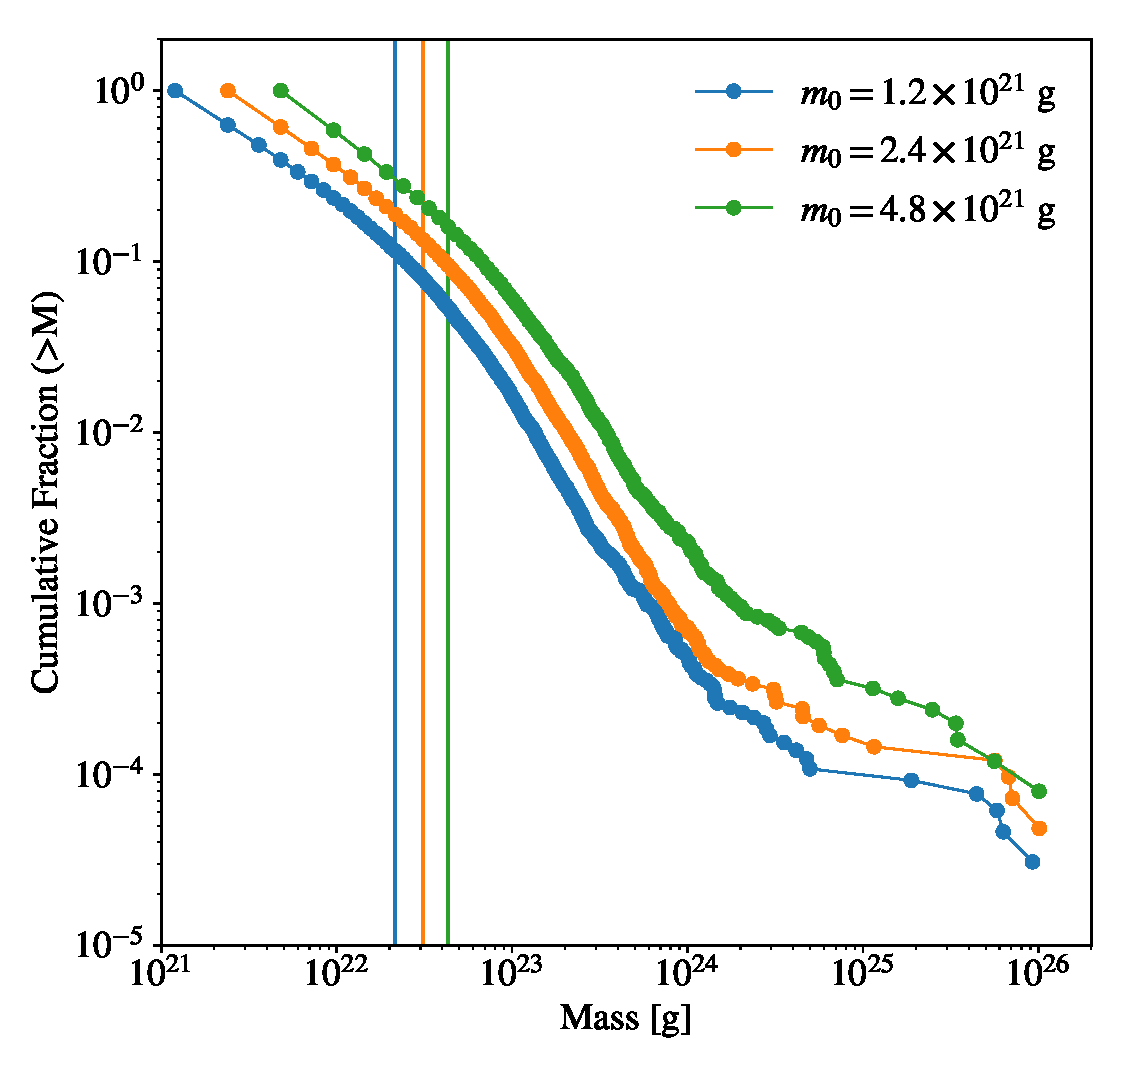
\includegraphics[width=\columnwidth]{figures/plSS/cum_model_comparison.eps}
    \caption{The cumulative mass distribution of planetesimals at the end of the three high-resolution growth simulations. The 
    vertical lines represent the mass at which the planetesimal spacing in semi major axis falls below the libration width of the 
    MMRs.}
    \label{fig:resolution_mass_dist}
\end{figure}

The size frequency distribution of asteroid belt objects is known to exhibit a power law break around around 
$1.05 \times 10^{21}$ g \cite{jedicke02}. The fact that the knee in the mass distribution is reproducible and appears sensitive to 
$m_{0}$ demonstrates that this value could be tuned to constrain planetesimal formation models by matching the observed 
mass of the bump with simulations. There is evidence that the shape of the SFD for asteroid belt objects more massive than 
about 100 km reflects that of the primordial population \cite{morbidelli09}. Although the purpose of this chapter is not to try to tune 
the model to match observations, we show the mass distribution from the $N=10^6$ growth simulation alongside the SFD of 
asteroid belt objects \cite{bottke05} in Figure \ref{fig:mass_dist_ast_compare} for comparison. Although the bump location in all 
of our simulations is larger than 100 km, a smaller initial planetesimal mass would probably produce a better match. The slope of 
the mass distribution above the bump mass matches reasonably well in both cases, but the slopes on the low mass end are 
discrepant. As the results from Figure \ref{fig:mass_spectrum_comp} show, a wider annulus tends to produce a shallower slope 
below the resonance heating mass. A better match might be made by simulating a wider annulus which includes resonances 
further from the embryos. Unfortunately, simulating an annulus wide enough to resolve all of the first order MMRs would require 
an extremely large number of particles.

As discussed in section \ref{sec:assumptions}, we do not expect the simplifying assumptions of perfect accretion and the 
absence of gas drag, along with the artificially inflated collision cross section to have a significant effect on the size distribution of 
accreted bodies. Because we have proposed that the initial planetesimal size could be reduced to better match the break in the 
asteroid belt SFD, we briefly consider the smallest sized planetesimals for which the resonant heating effect is not damped by 
gas drag. This will occur when the synodic period of the resonance becomes comparable to the stopping time. The latter quantity 
is given by equation \ref{eq:t_stop} and scales linearly with planetesimal size. For 100 km planetesimals, we showed that the 
stopping time is around $10^4$ years. The stopping time becomes comparable to the synodic period for bodies smaller than a 
few km in size, at which point \textbf{the resonant heating mechanism should no longer operate}.

\section{Summary and Discussion} \label{sec:discussion}

We have revealed a new mode of growth during the planetesimal accretion phase by simulating the interaction between 
oligarchs and planetesimals at unprecedented resolution. Shortly after the onset of oligarchic growth, a bump develops in the 
mass distribution of planetesimals. Below the bump mass, the surface density of planetesimals follows a shallower power law 
distribution. The break occurs near the mass at which the radial spacing of planetesimal matches the libration width of first order 
mean motion resonances with the oligarchs. These resonances, which are preferentially populated by the more numerous low 
mass planetesimals, act as effective pathways for dynamical friction to transfer energy and angular momentum from the 
oligarchs to the planetesimals. This result is analogous to the resolution dependence that \cite{weinberg07a, weinberg07b} 
found when examining the interaction between the bar and halo of a galaxy. This also matches the results of \cite{obrien06} and 
\cite{cionco02}, which showed that finer granularity in a planetesimal disc increases the effectiveness of dynamical friction. 
Bodies below the bump mass, which are packed tightly enough together to populate the resonances receive a disproportionate 
amount of energy and angular momentum from the oligarchs. Because this happens when the disc is hot enough to render 
gravitational focusing ineffective, this enhances the growth of the smallest planetesimals and produces a bend in the mass 
distribution.

Additionally, we ran a high resolution planetesimal growth simulation in which the width of the annulus was limited to exclude 
some of the resonances. Doing so mostly suppressed the formation of the bump near the resonance heating mass, although it 
did not completely get rid of it. We attribute this to the fact that we cannot make the annulus narrow enough to exclude all of the 
important resonances without introducing strong boundary effects which interfere with planetesimal growth. The fact that the 
feature in the mass distribution was greatly diminished when the many of the resonances were excluded is strong evidence that 
the MMRs are responsible for creating this bump.

\begin{figure}
    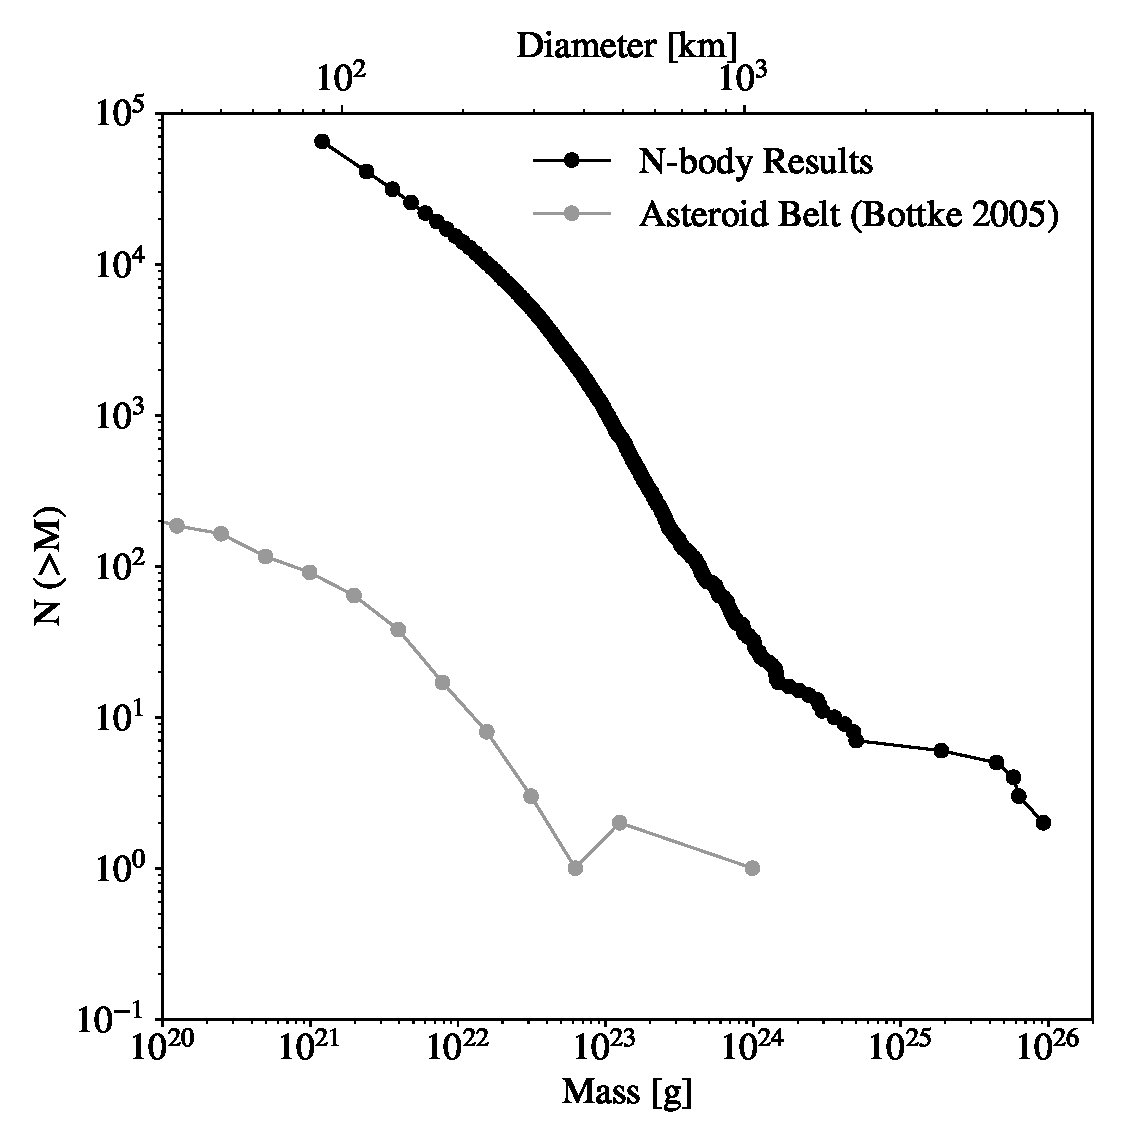
\includegraphics[width=\columnwidth]{figures/plSS/cum_asteroid_comparison.eps}
    \caption{A comparison between the cumulative number of objects in our high resolution growth simulation (black curve) and 
    the present day asteroid belt \cite{bottke05} (gray curve) as a function of size and mass.}
    \label{fig:mass_dist_ast_compare}
\end{figure}

% TODO: Figure too large

We confirmed this dynamical effect by placing a massive oligarch into a smoothly varying distribution of planetesimal masses. 
Within a few thousand orbits, the low mass planetesimals sitting within the zone of influence of the resonances began to migrate 
outwards, leaving a dearth of low mass bodies around the embryo. This effect did not appear when we simulated a similar 
heterogeneous distribution of masses, but limited the width of the annulus to exclude many of the MMRs. Additionally, the 
eccentricity of the oligarch decreased much more quickly when placed in a finely resolved disc with populated MMRs.

This result is significant because it suggests a new potentially observable link between the planetesimal formation process and 
the residual population of planetesimals in the present day Solar System. We showed that the mass distribution in our highest 
resolution simulation looks qualitatively similar to the SFD of objects in the asteroid belt, which, for objects larger than $\approx$ 
100 km, reflects the population of planetesimals at the end of the accretion stage \cite{morbidelli09}. We demonstrated that 
tuning the initial planetesimal mass in our simulation changes the location of the bump. This could potentially be matched with 
the observed 100 km feature in the asteroid belt to constrain planetesimal formation models. Additionally, using a wider annulus, 
which populates more of the first order MMRs, tends to produce a shallower slope on the low mass end of the mass distribution, 
which matches more closely with observations.

As discussed in section \ref{sec:bump}, there are a couple of explanations for this bump feature which were obtained from 
statistical models of planetesimal coagulation. It is unlikely that this resonance heating effect would naturally emerge from a 
statistical growth model unless it was explicitly built in. For this reason, this resonance heating effect has likely not been 
considered before. To our knowledge, no one has ever run an N-body simulation of planetesimal accretion to the oligarchic 
growth phase at this resolution.

Our results show that a feature similar to the power law break in the size distribution of asteroid belt objects can be produced 
without the effects of fragmentation, in contrast to \cite{morbidelli09}. Although our model does not account for the effects of 
fragmentation, the statistics of collisions above and below the bump mass are quite similar. We do not expect that including the 
effects of collisional fragmentation would significantly affect the location or strength of the bump. Regardless, these results 
demonstrate that a careful treatment of the dynamics is necessary to properly model planetesimal accretion during the oligarchic 
growth phase.

% TODO: Rory comment. Make appendices sections

\section{Appendix A: Mean Motion Resonance Test}

To demonstrate that {\sc ChaNGa} can properly track the motions of bodies in a mean motion resonance over many orbits, we 
present a test case with a central star, a perturbing massive body and a planetesimal. Although the simulations presented in this 
chapter are far more complex than this three body setup, the resonant interactions that produce the bump in the mass distribution 
are driven by the most massive bodies in the simulation. Because there are only a handful of these massive bodies, the tree 
approximation should have a negligible effect on the force contribution from these objects. For this reason, the behavior shown 
here should also apply to the previously presented simulations of planetesimal growth.

To test that the resonant interaction evolves correctly, we follow the evolution of the planetesimal in the complex x-y plane 
defined by the variable \cite{duncan89}

\begin{equation}\label{eq:complex}
    z = \left(G M_{*} a\right)^{1 / 4}\left\{2\left[1-\left(1-e^{2}\right)^{1 / 2}\right]\right\}^{1 / 2} \exp \left[i(\overline{\omega}-\lambda)\right],
\end{equation}

\noindent where a, e, $\overline{\omega}$ and $\lambda$ are the semi-major axis, eccentricity, longitude of perihelion and mean 
longitude of the planetesimal. If these values are recorded at the moment of opposition between the perturber and the 
planetesimal ($\lambda - \lambda_{p} = \pi$), the trajectory of the planetesimal should trace out a closed loop in the x-y plane. 
This indicates that an approximate Hamiltonian of the system is preserved and the resonant interaction is properly accounted for.

Figure \ref{fig:threebody} shows the evolution of the planetesimal over 20,000 years (about 130 synodic periods) in the complex 
x-y plane. The orbital elements of the planetesimal at the exact moment of opposition are calculated via linear interpolation. The 
perturbing body is placed at 1 AU on a circular orbit and has a mass of $10^{26}$ g, which is similar to the final mass of the 
embryos presented in simulation (i). The planetesimal is given a mass of $1.2 \times 10^{22}$ g and is placed on a coplanar 
orbit with a semi-major axis of 0.95501, which corresponds to the nominal location of the 15:14 mean motion resonance with the 
perturber. To start the planetesimal in a stable equilibirum, its orbital eccentricity is set to $10^{-2}$ so that the longitude of 
pericenter is well-defined. Fixed timesteps of $\Delta$T = 0.0025 yrs are taken, which is the same as the previous simulations. In 
this configuration, the Jacobi constant is small and so the planetesimal follows a circular trajectory in the complex plane. 
Because the perturbing body is on a circular orbit, the forced eccentricity is zero and the trajectory of the planetesimal is 
centered at the origin. Most importantly, trajectory of the planetesimal appears to follow a closed loop, which indicates that an 
approximate Hamiltonian is preserved and the integration is accurate enough to follow mean motion resonances in this 
configuration.

\begin{figure}
    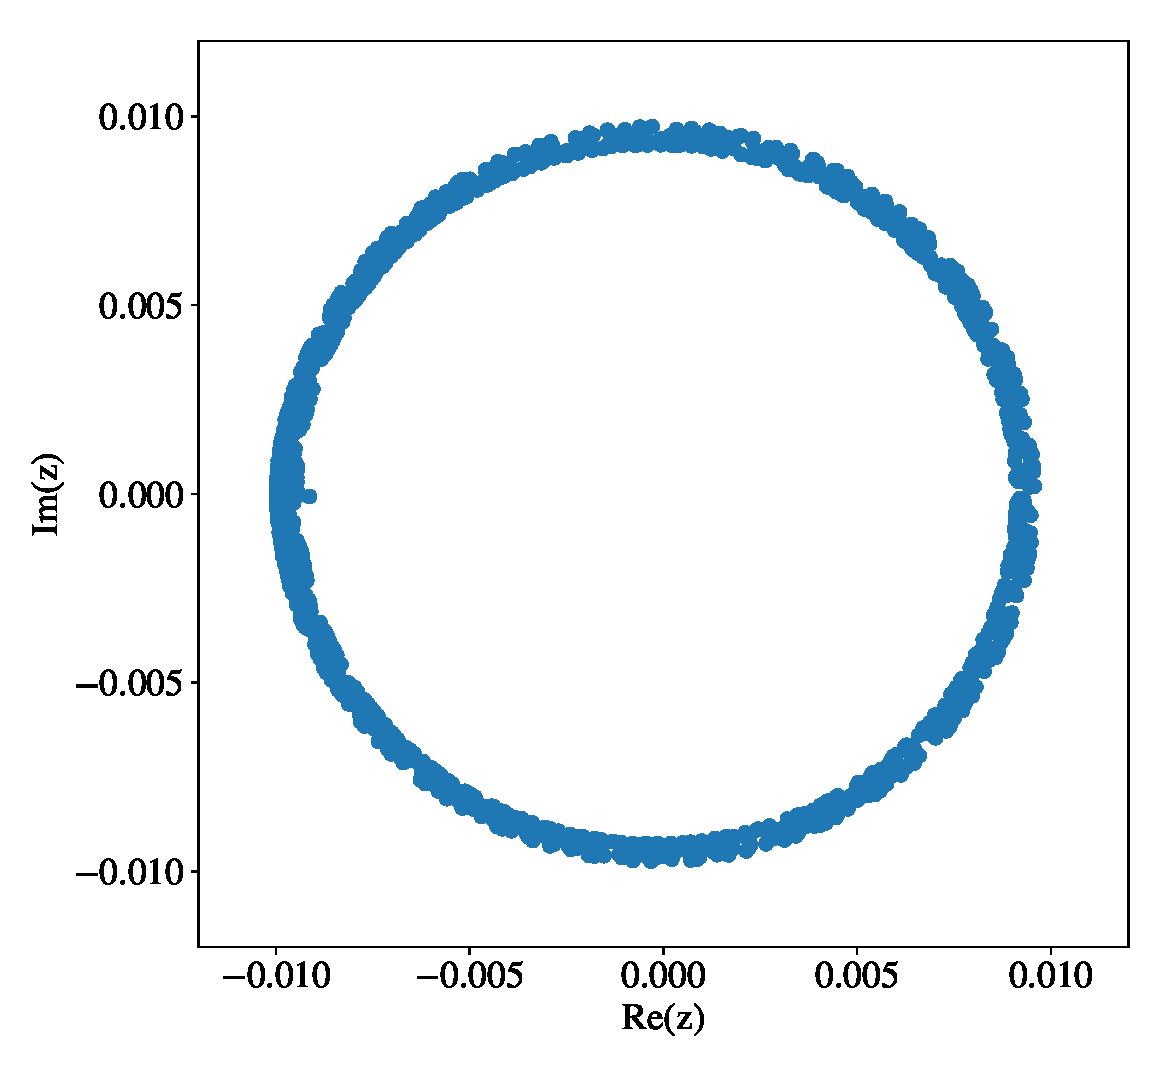
\includegraphics[width=\columnwidth]{figures/plSS/threebody_complex.eps}
    \caption{The evolution of the planetesimal in the complex plane defined by equation \ref{eq:complex}. Each point represents 
    the state of the system when the perturber and planetesimal are at opposition.}
    \label{fig:threebody}
\end{figure}

\begin{figure*}
    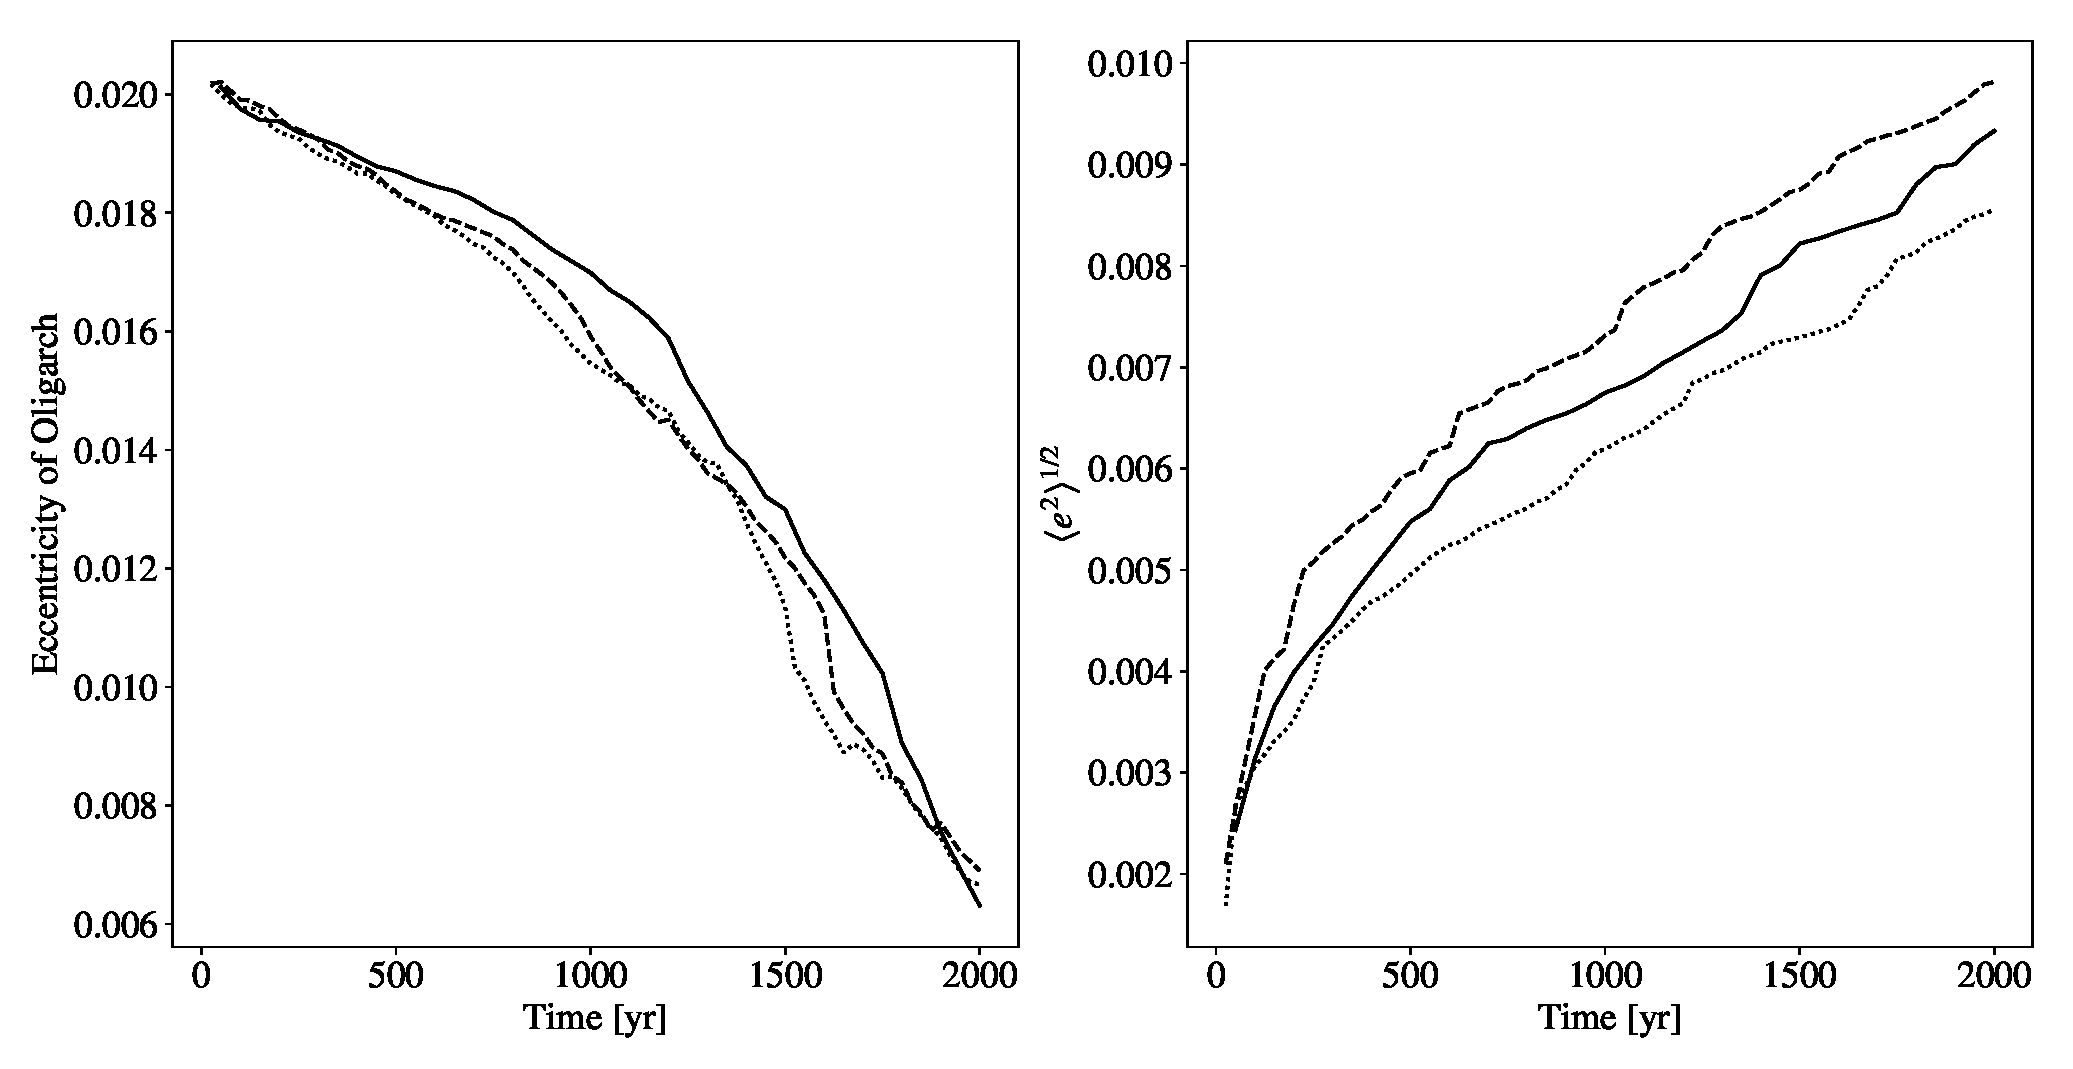
\includegraphics[width=\textwidth]{figures/plSS/theta_test.eps}
    \caption{Time evolution of the eccentricity of the oligarch (left) and rms eccentricity of the smallest planetesimals (right) in the 
    $e_{hi}$ simulation with an opening angle $\Theta_{BH}$ of 0.7 (solid line) and 0.35 (dashed line). The dotted line shows 
    $\Theta_{BH}$ = 0.7 with a timestep that is half as large.}
    \label{fig:theta_test}
\end{figure*}

\section{Appendix B: Tree Approximation and Opening Angle}\label{sec:openAngle}

The results we have presented in this work depend on repeated two-body interactions between planetesimals. As discussed in 
section \ref{sec:assumptions}, the location of the bump in the mass spectrum depends on the amount of viscous stirring that 
has occurred before oligarchic growth commences. Additionally, the resonant heating effect presented in this work requires that 
viscous stirring is not too vigorous as to prevent repeated conjunctions. Here, we examine the impact of force calculation errors 
from our tree algorithm on these phenomena.

{\sc ChaNGa} calculates the gravitational interaction force between particles via a tree approximation. Particles that only weakly 
contribute to the gravitational potential are grouped together during the force calculation phase. The opening angle $\Theta$ 
controls how likely particles are to get grouped together during this stage. Because the lowest mass particles contribute weakly 
to the surrounding potential, the gravitational contribution from these bodies is more approximate. This can potentially alter the 
effectiveness of viscous stirring. For this reason, we re-ran the $e_{hi}$ simulation with a smaller, more restrictive opening 
angle of $\Theta_{BH}$ = 0.35 to test whether the tree approximation is noticeably altering the behavior of viscous stirring. 
Because we expand forces from tree nodes to hexadecapole order, an opening angle that is a factor of 2 smaller should reduce 
the error in the force calculations by a factor of 16. Additionally, we test $\Theta_{BH} = 0.7$ with a timestep of $\Delta T$ = 
0.00125 years.

A comparison between the three versions of the $e_{hi}$ simulation is shown in Figure \ref{fig:theta_test}. In all cases, the 
oligarch slowly loses eccentricity for about 1000 years before the curve drops more steeply. With a smaller opening angle or a 
smaller timestep size, the downturn appears to happen slightly sooner. By the end of the simulation, the resulting eccentricities 
of the oligarchs are still within 10 percent of each other. The right hand panel of Figure \ref{fig:theta_test} shows the evolution of 
the rms eccentricity of the lowest mass planetesimals. There is some divergence between the curves early on, but this only 
lasts for a fraction of the viscous stirring timescale. As was shown in section \ref{sec:assumptions}, it would take a much larger 
difference in the rms eccentricity than is seen here here to alter the bump in the mass spectrum. The evolution of the rms 
inclination of the planetesimals is qualitatively similar in all three cases.
\chapter {Detecting Cold Jupiters via Collisional Grinding of Planetesimals}\label{ch:grind}

\noindent \textit{The content of this chapter was originally published in collaboration with Thomas R. Quinn and Aaron C. Boley in the June 2021 edition of The Monthly Notices of the Royal Astronomical Society (\cite{wallace21}, MNRAS, Vol. 503, 4; 2011, DOI: 10.1093/mnras/stab792), and is reproduced below with the permission of the Royal Astronomical Society.}

\section{Introduction} \label{sec:intro}

Recent observations of circumstellar discs by ALMA have revealed a rich variety of substructure. Features such as gaps and 
asymmetries \cite{alma15, perez16, isella16, andrews16, cieza16} in the emission provide diagnostics for the physical 
processes that drive the evolution of the discs. In many gas-rich systems, these gap features are argued to indicate the 
presence of a giant planet, either embedded in the disc \cite{dipierro15} or orbiting adjacent to it, although the details of gas-dust 
interactions can have strong effects on the resulting morphologies \cite{dong18}. In gas-poor/debris systems, a giantplanet 
perturber can also influence the structure of the dust continuum emission. For example, a misaligned giant planet can produce 
nonaxisymmetric features such as warps \cite{augereau01}, highly eccentric perturbers can produce structures through secular 
interactions \cite{pearce14, pearce15}, and mean motion resonances (MMRs) can open gaps
\cite{nesvold15, tabeshian16, tabeshian18}.

Collisions between planetesimals are thought to be the principal source of dust for debris discs (see \cite{wyatt08}).  Although 
some amount of primordial dust is likely still present during the early stages of debris disc evolution, ongoing collisions between 
small bodies will augment this and could be used to trace the underlying dynamical activity of the planetesimals. This process 
was directly detected when the putative object Fomalhaut b was confirmed to be an expanding debris cloud, most likely from a 
planetesimal collision \cite{gaspar20}. 

\cite{dobinson13} showed that collisional dust that is generated near the gap opened by a giant planet in the inner regions of a 
transition disc should produce a distinct observable marker that could be used to infer the presence of the planet. In a followup 
study, it was found that morphological differences in the dust emission could be used to determine whether the planet had a 
circular or eccentric orbit \cite{dobinson16}. Moreover, substructure due to mean-motion resonances (MMRs) with a giant planet 
may hold additional clues that could be used to constrain the properties of the planet.  The width of a resonance is set by both 
the mass of the perturbing planet and the unperturbed eccentricity of the planetesimals, which is in turn set by the eccentricity of 
the planet through secular forcing. Therefore, the planetesimal collision profile and potentially the structure of second generation 
dust produced near MMRs may encode information about both the mass and eccentricity of the planet.

The dynamics governing the motion of bodies near MMRs is extremely nonlinear, as is determining what the collision rates 
between planetesimals should look like in these regions. For a collection of bodies massive enough to experience the effects of 
gravitational focusing, a large eccentricity dispersion tends to reduce the probability of collision, while enhancements in surface 
density tends to increase it. Due to conservation of the Jacobi energy, MMRs simultaneously enhance the local eccentricity 
dispersion and also enhance the surface density adjacent to the resonance \cite{richardson00, boley17}. Unfortunately, collision 
detection in an N-body simulation is extremely computationally expensive. So far, studies of planetesimal dynamics near MMRs 
in which the planetesimals are directly resolved have involved either collisionless test particles 
\cite{boley17, tabeshian16, tabeshian18} or integration times that do not fully capture the dynamics of the resonances 
\cite{richardson00, dobinson13}.

To further elucidate this subject, we use the tree based N-body code {\sc ChaNGa} \cite{jetley08, menon15} to follow the 
collisional evolution of a planetesimal disc under the gravitational influence of a Jupiter-sized body. Because particle positions 
are sorted into a tree structure, neighbor finding and collision detection can be done quickly and efficiently. This considerably 
relaxes the constraints on resolution and integration time. With this toolset, we explore the collision rate structure of a 
planetesimal disc in the vicinity of mean-motion resonances with a planet. In particular, we would like to determine (1) what 
dynamics govern the collision rate profile near MMRs, (2) whether MMRs leave a detectable signature in thecollisionally-
generated dust, and (3) whether these signatures can be used to determine or constrain the orbital properties of the perturbing 
planet.

This work is organized in the following way: In section \ref{sec:dynamics}, we provide an overview of the relevant dynamics that 
drive the evolution of a planetesimal disc under the gravitational influence of an external perturber. In section \ref{sec:sims} we 
provide an overview of the N-body code used and describe the initial conditions chosen for five simulations in which a perturbing 
giant planet is given various masses  and eccentricities. Section\ref{sec:results} presents the results of these simulations and we 
take an in-depth look at the collision rate profiles of the planetesimals near the MMRs. In section \ref{sec:dust},  we extrapolate 
the collision rate down to smaller bodies and motivate a direct correspondence between the planetesimal collision profile and the 
resulting dust profile. In section \ref{sec:constrain}, we use the resolved collisions to generate synthetic dust emission profiles 
that would be detected with observing facilities like ALMA. Under our simplifying assumptions, we show that a characteristic 
bump or dip feature appears in the dust emission near the interior 2:1 MMR, the presence of which depends on the mass and 
eccentricity of the perturbing planet. If the 2:1 MMR can be identified (presumably, by identifying another prominent MMR, such 
as the 3:1, and measuring the spacing between the two), we discuss the potential for using this feature to place constraints on 
the mass and eccentricity of the planet. In addition, we highlight the caveats of connecting the dust and planetesimal collision 
profiles in such a simple way. Finally, we conclude in section \ref{sec:conclusions}.

\section{Overview of Relevant Dynamics} \label{sec:dynamics}

We begin by providing a description of the dynamical effects responsible for shaping the orbital distribution of the planetesimals. 
The purpose of this is twofold: (1) to motivate the initial conditions used for the simulations described in section \ref{sec:ics} and 
(2) to justify the exclusion of certain physical effects from our simulations. Here, we focus solely on the physics relevant for full-
sized ($\sim$100 km) planeteismals and save a discussion of the effects on smaller bodies generated through collisions for 
section \ref{sec:dust}.

\subsection{Secular Forcing}\label{sec:sec_force}

The most direct and widespread effect that a perturbing giant planet will have on a planetesimal disc is through secular forcing of 
the planetesimals. This will cause the complex eccentricities of the planetesimals to take on a time-independent forced value, 
given by \cite{wyatt99} as

\begin{equation}\label{eq:eforced}
	z_{f} = \frac{b^{2}_{3/2} (\alpha)}{b^{1}_{3/2} (\alpha)} e_{g} ~ \mathrm{exp} ~ i \varpi_{g}.
\end{equation}

\noindent Here, $\alpha = a_{g} / a$ where $a_{g}$ and $a$ are the semi-major axes of the giant planet and a planetesimal, 
respectively. $e_{g}$ and $\varpi_{g}$ are the eccentricity andlongitude of pericenter of the giant planet, and $b^{j}_{s} (\alpha)$ 
is a Laplace coefficient given by \cite{murray99} (ch. 6, pg. 237, eq. 6.67) as

\begin{equation}\label{eq:lap}
	b_{s}^{j}(\alpha) = \frac{1}{\pi} \int_{0}^{2 \pi} \frac{\cos \, j \psi \, d \psi}{\left( 1 - 2 \alpha \, \cos \psi + \alpha^2 \right)^{s}}.
\end{equation}

Without any nearby secular or mean motion-resonances, equation \ref{eq:eforced} will completely describe the eccentricities and 
longitude of  pericenter orientations of the planetesimals. Additional forces due to two-body scattering between planetesimals, 
along with aerodynamic gas drag will add an additional free component to the complex eccentricity, which will be randomly 
oriented. The magnitude of the free eccentricity describes how dynamically hot the planetesimal disc is and sets the random 
encounter speeds of planetesimals. When the dynamical excitation of the disc is driven by gravitational stirring, the magnitude of 
the free eccentricity can be described by a Rayleigh distribution \cite{ida92}.

For the case of a Jupiter mass planet at 5.2 au perturbing a test particle at 3 au, the timescale for secular forcing is 
approximately 12,000 years. The details of this calculation can be found in appendix \ref{sec:sec_forcing_timescale}.

\subsection{Mean-Motion Resonances}\label{sec:mmr}

In regions where there are commensurabilities between frequencies, Laplace-Langrange secular theory breaks down and bodies 
are subject to strong perturbations. For the purposes of this study, we will ignore secular resonances, which generally occur on 
rather large timescales and will focus on mean-motion resonances. A MMR occurs  when the orbital period ratio between two 
bodies is sufficiently close to

\begin{equation}\label{eq:per_mmr}
	\frac{P}{P'} = \frac{p + q}{p},
\end{equation}

\noindent where  $p$ and $q$ are integers $>$ 0 and the unprimed and primed quantities correspond to the perturber and the 
body being perturbed, respectively. In terms of these quantities, $P/P'$ corresponds to a $p+q:p$ resonance. If the perturber is 
much more massive than the other body and all of the bodies lie in a near-Keplerian potential, the condition for MMR is set by

\begin{equation}\label{eq:a_mmr}
	\frac{a}{a'} = \left( \frac{p}{p + q} \right)^{2/3}.
\end{equation}

If we further assume that the two bodies are orbiting in the same plane, the motion of the bodies near resonance is determined 
by the behavior of a critical angle

\begin{equation}\label{eq:phi_crit}
	\phi = (p + q) \lambda' - p \lambda - q \varpi,
\end{equation}

\noindent where $\lambda = \varpi + M$ is the mean longitude of abody, with $M$ being the mean anomaly. For bodies in 
resonance, the critical angle will librate around an equlibrium value, while this angle will circulate outside of resonance. For small 
eccentricities, this behavior is analogous to the motion of a pendulum. Furthermore, variations in the critical angle are coupled to 
changes in the mean motion and semimajor axis \cite{murray99}. An important point to note, which we will revisit later, is that the 
variation frequency of this angle approaches zero near the edge of a resonance. The width of a resonance can be defined by 
determining the largest variation in semimajor axis that permits librational, rather than circulatory motion of $\phi$. Calculations 
for the widths of first and second order interior MMRs are shown in appendix \ref{sec:libration}, along with a timescale for the 
libration. For the most prominent interior mean-motion resonances, including the 2:1 and 3:1, the timescale associated with 
these oscillations driven by a Jupiter mass planet is  $\sim$ 1,000 - 2,000 years.

\subsection{Collisions Between Planetesimals}\label{sec:colleq}

A simple analytic model for the collision rate of a planetesimal population is given by \cite{safronov69} as

\begin{equation}\label{eq:saf}
	n \sigma v = n \pi s^{2} \left( 1 + 2 G m / s v^{2} \right) v,
\end{equation}

\noindent where $n$ is the number density of the population, $s$ and $m$ are the radii and masses of the bodies and $v$ is 
their typical encounter velocity. The encounter velocity is often described in terms of the rms eccentricity 
$\left<e^{2}\right>^{1/2}$ and inclination $\left<i^{2}\right>^{1/2}$ of the population (e.g. \cite{lissauer93}) as

\begin{equation}\label{eq:eccincvel}
	v = \sqrt{\left< e^{2} \right> + \left< i^{2} \right>} v_{k},
\end{equation}

\noindent where $v_{k}$ is the local Keplerian velocity. The second term in equation \ref{eq:saf} can be thought of as an 
additional enhancement to the collision cross section due to gravitational focusing. When the typical encounter velocity is small 
compared to the mutual escape velocity of the planetesimals, the collision cross section greatly exceeds the geometric value. An 
important feature of equation \ref{eq:saf} is that for a fixed value of $n$, the collision rate exhibits a global minimum as a function 
of $v$. For small $v$, gravitational focusing facilitates more collisions, while for large $v$ the encounter rate simply becomes so 
great that the collision rate again increases, even though gravitational focusing is mostly suppressed. This point will become 
relevant in section \ref{sec:vary_ecc} when we examine the qualitative changes in the collision rate near mean-motion 
resonances.

Although equation \ref{eq:saf} works well to describe the collision rate for a homogeneous collection of planetesimals, some 
problems arise when regions of commensurabilities are introduced. Namely, the resonances cause the orbits of planetesimals to 
precess, and an interface between secularly aligned and randomly oriented orbits arise on each side of the resonance. 
Additionally, an interface between dynamically cold and hot planetesimals develop. These two effects cause the number density, 
collision cross section and encounter velocity to rather abruptly vary across the boundaries of the resonance. For this reason, an 
N-body treatment in which collisions are directly resolved is necessary to understand how the collision rate varies near the 
MMRs.

\subsection{Gas Drag on Planetesimals}\label{sec:pl_drag}

Over the course of many orbits, the residual gas from the primordial nebula can damp the eccentricities and inclinations of 
bodies. For a planetesimal-sized body, gas drag operates in the Stokes regime and the timescale for aerodynamic forces to 
significantly alter its relative velocity is given by \cite{adachi76}

\begin{equation}\label{eq:ts_stokes}
    t_{s} = \frac{2 m}{C_{D} \pi s^{2} \rho_{g} v_{g}},
\end{equation}

\noindent where $m$ and $s$ are the mass and radius of the planetesimal. $C_{D}$ is a drag coefficient which is of order unity, 
$\rho_{g}$ is the local density of the gas and $v_{g}$ is the headwind velocity of the gas experienced by the planetesimal. At 3 
au, the gaseous component of the solar nebula has a density of $3 \times 10^{-11}$ g cm$^{-3}$ and the typical headwind 
experienced by a body on a Keplerian orbit is $\sim 5,000$ cm s$^{-1}$ \cite{hayashi81}. For a 100 km body with a density of 2 g 
cm$^{-3}$ (assuming a mixture of ice and rock) the stopping timescale is about 1 Myr. This is much longer than the timescales 
associated with secular forcing and libration due to mean-motion resonances, as discussed above, but shorter than the typical 
protoplanetary disk lifetime and potentially shorter the planetesimal formation timescale. For this reason, we do not model the 
effects of gas drag in the simulations, although we consider its effects when constructing initial conditions, which is discussed in 
the next section.

\begin{figure*}
\begin{center}
    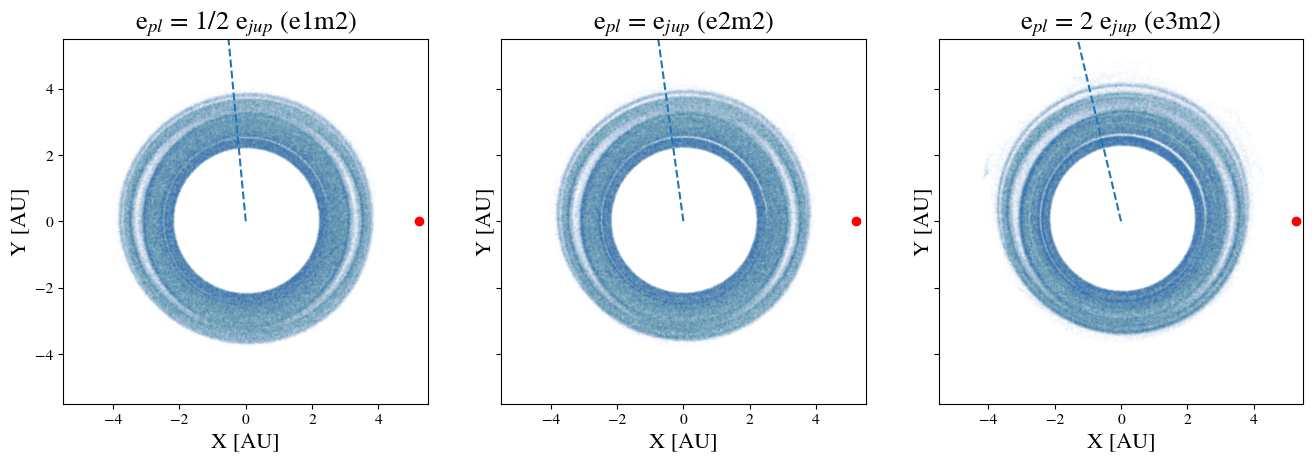
\includegraphics[width=\textwidth]{figures/grind/xy.png}
    \caption{The positions of the remaining planetesimals at the end of the e1m2 (left), e2m2 (center) and e3m2 (right) 
    simulations. The red dot indicates the position of the giant planet, and the dashed line points in the direction of the planet's 
    longitude of perihelion. Non-axisymmetric gaps are apparent near the locations of MMRs. At higher eccentricities, more 
    resonances become visible. At the 2:1 MMR, gap features at $\theta$ = 0 
    and $\theta = \pi$ follow the giant planet in its orbit.\label{fig:xy}}
\end{center}
\end{figure*}

\section{Simulations} \label{sec:sims}

\subsection{Numerical Methods}\label{sec:methods}

To follow the dynamical and collisional evolution of a planetesimal disc, we use the highly parallel N-body code {\sc ChaNGa}. A full 
description of the code, along with the details of the solid body collision module are provided in chapter \ref{ch:intro}. During the course 
of the simulation, no debris is created by collisions. To model the collisionally generated dust distribution, we use the statistics of the 
resolved planetesimal collisions to build a dust profile. This process is discussed in detail in section \ref{sec:dust}.

\begin{table}
\begin{center}
\caption{Summary of Simulations Run}
\begin{tabular}{lllll} \hline \hline
Name     & Mass of Planet & Eccentricity of Planet &  &  \\ \hline
e1m2 & 1.0 $M_{jup}$                     & 0.5 $e_{jup}$                            &  &  \\
e2m2      & 1.0 $M_{jup}$                     & 1.0 $e_{jup}$                             &  &  \\
e3m2 & 1.0 $M_{jup}$                     & 2.0 $e_{jup}$                             &  &  \\
e2m1 & 0.5 $M_{jup}$                   & 1.0 $e_{jup}$                             &  &  \\
e2m3 & 2.0 $M_{jup}$                     & 1.0 $e_{jup}$                             &  &  \\ \hline
\end{tabular}
\label{tab:sims}
\end{center}
\end{table}

\subsection{Initial Conditions}\label{sec:ics}

In total, five simulations are run, which are listed in table \ref{tab:sims}. The second is a ``nominal'' case, in which the perturbing 
planet's mass and eccentricity are set to that of Jupiter's. In the other four cases, the mass or eccentricity is altered by a factor of 
two from the nominal value. In all cases, the perturbing giant is placed on a 5.2 au orbit around a 1 $M_{\odot}$ star. The 
planetesimal disc extends from 2.2 to 3.8 au, which covers the two most prominent mean-motion resonances with the giant 
planet, the 2:1 at 3.27 au and the 3:1 at 2.5 au. The planetesimal disc loosely follows a minimum-mass solar nebula surface 
density profile \cite{hayashi81}

\begin{equation}\label{eq:surf_den}
	\Sigma = \Sigma_{0} r^{-\alpha},
\end{equation}

\noindent with $\alpha$ = 3/2 and $\Sigma_{0}$ = 10 g cm$^{-2}$. Planetesimals are given a bulk density of 2 g cm$^{-3}$, 
which corresponds to a mixture of ice and rock, and are given a diameter of 300 km. This choice of parameters is meant to 
mimic the setup used in simulation B from \cite{richardson00}. One difference from the aformentioned study is that we use a 
narrower annulus, which reduces the number of particles required from $10^6$ down to roughly 500,000. This allows us to use a 
finer base timestep size, which, as we will discuss in section \ref{sec:results}, appears to be the reason why no features were 
seen in the collision profile near the resonances by \cite{richardson00}.

Another difference from \cite{richardson00} is that the dynamical effects of secular forcing by the giant planet, along with the 
effects of viscous stirring and gas drag on the planetesimals, are built into the initial conditions. Although we do not model the 
effects of gas drag on the planetesimals during the simulation, we construct the initial conditions such that the effects of gas drag 
and viscous stirring are in balance. The viscous stirring timescale of the planetesimal disc is much longer than our chosen 
integration time, and so the dynamical excitation of the disc (excluding resonances) stays constant, even without the inclusion of 
damping forces from the gas. This is done by first calculating the equilibrium eccentricity $e_{eq}$ due to viscous stirring and 
gas drag as a function of semimajor axis according to equation 12 of \cite{kokubo02}. The eccentricities of the bodies are drawn 
randomly from a Rayleigh distribution with a mode of $e_{eq}$, while the inclinations are drawn from a similar distribution with a 
mode of $e_{eq}$/2 \cite{ida93a}. The arguments of perihelion $\omega$, longitude of ascending nodes $\Omega$ and the 
mean anomalies $M$ of the bodies are drawn uniformly $\in [0, 2 \pi)$.

To account for the effects of secular forcing by the planet, the eccentricity vectors of the planetesimals are first decomposed into 
real and imaginary components:

\begin{equation}\label{eq:kh}
	z = (k, ih) = e \, exp(i \varpi)
\end{equation}

\noindent and a forced component is added to $h$ according to equation \ref{eq:eforced} (where we have set $\varpi_{g}$ = 0).

\subsection{Time Stepping Scheme}\label{sec:timestep}

For the purposes of the integrator, there are two relevant timescales in this system. The first is the orbital dynamical time 
$\sqrt{a^3/G M_{\odot}}$. Through experimentation, we have found that using a base timestep size with {\sc ChaNGa} of 3\% of 
an orbital dynamical timeat the inner edge of the disc keeps the integration symplectic. Although doing so preserves orbital 
frequencies, the errors associated withprecession frequencies do not average out to zero. This is especially important given the 
effects of secular forcing by the planet. To mitigatethis, we further reduce the base timestep size by a factor of 4 and use $\Delta 
t$ = 0.0025 yr. Doing so prevents the longitude of perihelia ofplanetesimals at the inner edge of the disc, where this artificial 
precession is most severe, from drifting by more than the intrinsic spread in $\varpi$ due to thefree eccentricity over the course 
of our integrations.

An additional timescale is set by the dynamical time of the planetesimals ($\sim 1/\sqrt{G \rho}$), which is about 45 minutes. This 
timescale must be resolved in order to properly follow close gravitational encounters between these bodies. To resolve the base 
time step and the dynamical timescale of planetesimals simultaneously, we use a two-tiered time stepping scheme, 
following\cite{leinhardt15}. To start, all bodies are placed on the base time step. A first pass of collision detection is then run in 
which the radii of all bodies are inflated by a factor of 2.5. Any bodies with imminent collisions predicted using the inflated radii 
are placed on a time step that is a factor of 16 smaller than the orbital time step. Although this is still a factor of roughly 7 larger 
than the dynamical time of a planetesimal, we found no difference in the collision rate when using any smaller of a minimum time 
step size.The purpose of the two-tiered scheme is to properly resolve the gravitational interactions between any bodies that 
undergo a close encounter. This prevents the coarser base time step from reducing the effectiveness of gravitational focusing, 
while minimizing the additional computational expense.

\begin{figure}
\begin{center}
    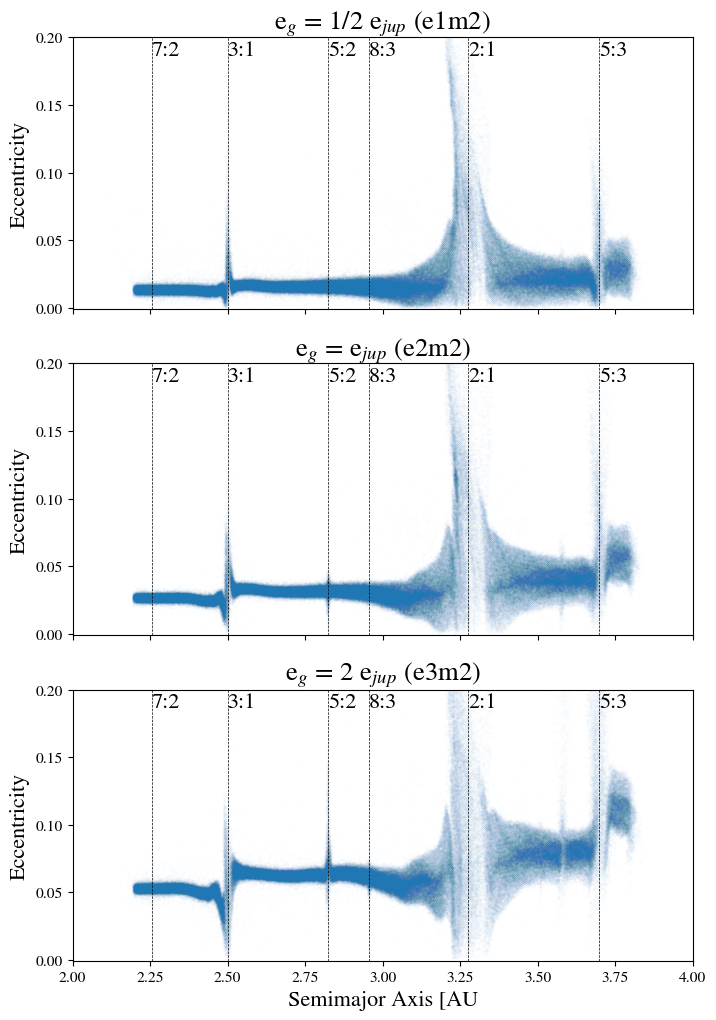
\includegraphics[width=0.5\textwidth]{figures/grind/ae.png}
    \caption{The semimajor axes and eccentricities of the remaining planetesimals are shown, with the locations of prominent 
    resonances indicated by the vertical dashed lines. Libration of the critical angle drives large variations in eccentricity, which 
    produce spikes in the a-e plane. Between the resonances, the nonzero eccentricity is due to secular forcing by the planet.
    \label{fig:ae}}
\end{center}
\end{figure}

\begin{figure*}
\begin{center}
    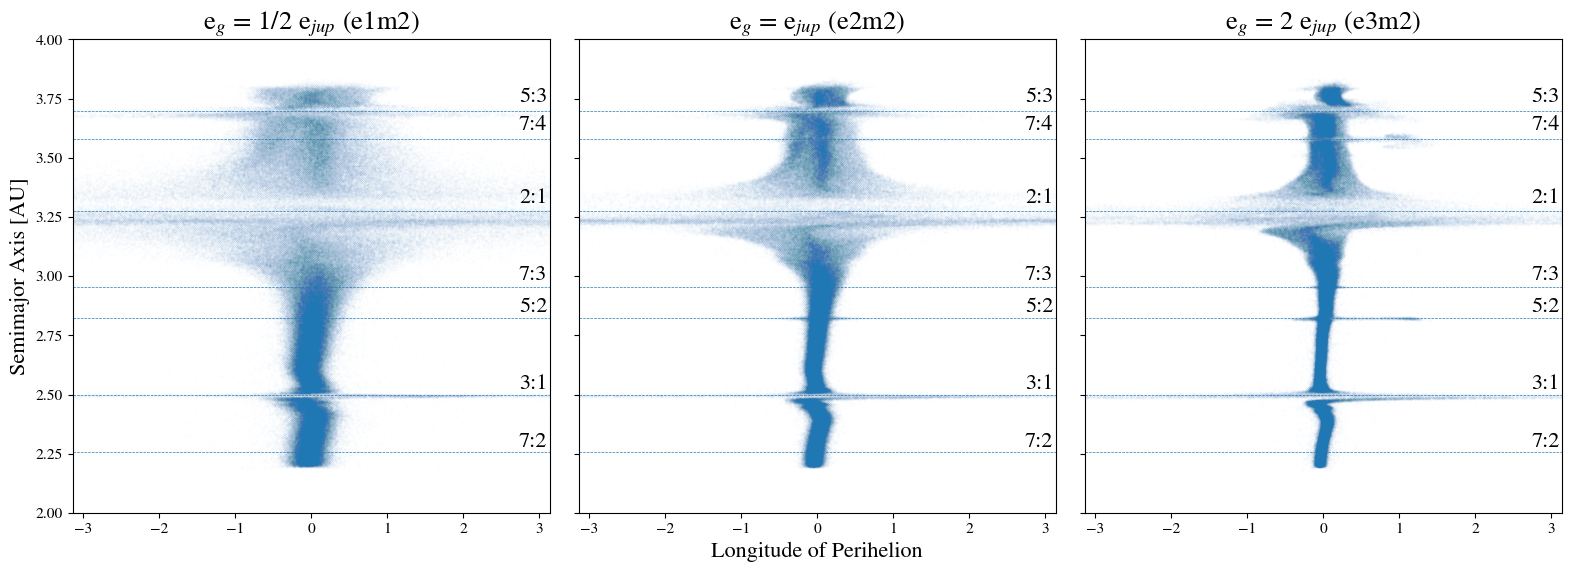
\includegraphics[width=\textwidth]{figures/grind/long_ph.png}
    \caption{Shown here are the longitudes of pericenter and semimajor axes of the remaining planetesimals. The dashed lines 
    again indicate the locations of prominent MMRs. Close to the resonances, the critical angle librates and drives fast precession 
    of the longitudes of pericenter of the bodies. This overpowers the secular forcing by the planet and effectively randomizes the 
    orientations of their orbits.\label{fig:long_ph}}
\end{center}
\end{figure*}

\section{Results} \label{sec:results}

All five simulations are evolved for 5,000 years, which is roughly 400 complete orbits of the perturbing planet. Because the 
effects of the mean motion resonances are not built into the initial conditions, the simulations must be run long enough for the 
distribution of orbital elements to reach equilibrium near the resonances before the collision rate is measured. To do so, we allow 
each simulation to run for 2,000 years before we begin recording any collision statistics. This is comparable to the libration 
period, which was calculated in section \ref{sec:mmr} for the 3:1 and 2:1 resonance. Although one might worry that a single 
libration period may not be long enough for the orbital structure due to the resonances to develop, we find that the shape of the 
semimajor axis-eccentricity distribution of the planetesimals reaches a steady state by this time. This is largely due to the fact 
that there are enough bodies in or near the resonances to allow an ensemble average of phase space, rather than a time 
average. As an additional confirmation, we find that the time evolution of the collision rate near the resonances maintains a 
steady state in all five simulations after $\sim$ 2000 years.

\subsection{Varying the Eccentricity} \label{sec:vary_ecc}

We begin by examining simulations e1m2, e2m2 and e3m2. The positions of the planetesimals in the x-y plane after 5,000 years 
of integration are shown in figure \ref{fig:xy}. In all cases, the coordinate system is rotated so that the giant planet lies at $\theta 
= 0$. The longitude of perihelion of the planet is shown by the dashed line. Resonances with the perturbing planet are visible as 
nonaxisymmetric gaps in this figure. Upon close inspection of a series of simulation snapshots, these gaps appear to follow the 
planet in its orbit, rather than aligning themselves with the longitude of perihelion. A similar substructure, which is most 
noticeable near the 2:1 MMR, reveals itself in \cite{richardson00} (see their figures 3c and 3f) and \cite{tabeshian16} (see their 
figure 3a). This structure is also present in the \cite{boley17} simulations, although it was not reported at the time (see Appendix 
\ref{sec:boley_plot}). It is worth noting that both \cite{richardson00} and \cite{boley17} started with a completely cold 
planetesimal disc. Thus, the presence of these features seems robust to the choice of initial conditions.

The effects of the resonances become much more apparent in semimajor axis-eccentricity space, which is shown in figure 
\ref{fig:ae}. In all cases, the 3:1, 2:1 and 5:3 resonances are readily visible as ``spikes'' in the eccentricity that bend slightly 
inward (due to the conservation of the Jacobi energy). In the e3m2 simulation, features also appear near the 5:2, 7:3 and 5:3 
resonances. The absence of these finer features from the e1m2 simulation can be explained by the fact that the strength of a 
resonance scales with $e^{q}$ \cite{malhotra94}.

Another important effect of the resonances is visible in figure \ref{fig:long_ph}, which shows the orientation of the longitude of 
perihelia of planetesimals in the disc. Inside of the resonances, orbits of planetesimals quickly precess, and their orientations are 
effectively randomized. An important point to note is that this strong precession effect quickly disappears beyond the boundaries 
of the resonance. This turns out to be key to explaining the nonaxisymmetric structure seen in figure \ref{fig:xy}, which will be 
addressed in more detail below.

Next, we examine the statistics of collisions resolved in each of the simulations. The 3D positions and velocities of the two 
colliding bodies are recorded to a table at the moment of impact. We derive the Keplerian orbital elements of a collision using 
these positions and velocities. First, we examine the semimajor axis of the first collider, which is shown in figure 
\ref{fig:coll_hist_a}. During a collision, the ``first'' particle is defined as the more massive of the two. However, nearly all of the 
collisions happen between the initial, equal-mass planetesimals. In this case, the distinction is set by the collision search 
algorithm and is rather arbitrary. In all of the plots where we show collision statistics, we have verified that using the ``first'' or 
``second'' collider does not qualitatively change any of the features. We find that some of the features present in figure 
\ref{fig:coll_hist_a} in this and subsequent figures are highly sensitive to the number of bins and the location of the bin edges. 
For this reason, we construct a probability density function (PDF) of the collisions using a Kernel Density Estimate (KDE). We 
use the {\sc neighbors.KernelDensity} function from the {\sc sklearn} \cite{scikit-learn} package to construct our KDEs, using a 
gaussian kernel with a FWHM of 0.02 au. The curves shown in figure \ref{fig:coll_hist_a} are normalized such that the area 
underneath is equal to 1.

Near the stronger resonances, there are noticeable suppressions or enhancements to the local collision rate. This contrasts with 
the findings of \cite{richardson00}, who simulated a similar setup and found no discernible features near the MMRs. We attribute 
the differences to a more conservative timestepping criterion in our simulations, along with the inclusion of secular perturbations 
in our initial conditions. The most prominent features appear as a local maximum in the collision rate near the 2:1 MMR and a 
local minimum near the 3:1 MMR. At higher forced eccentricities, features near the 5:2, 8:3 and 5:3 resonances are also visible, 
due to the steep sensitivity of higher order resonant perturbations to eccentricity \cite{malhotra94}.

Although the features in figure \ref{fig:coll_hist_a} near the 3:1 and 2:1 MMRs appear qualitatively different, they can be 
explained by one single dynamical process. As discussed in section \ref{sec:colleq}, the collision rate between planetesimals 
depends on both the encounter rate and the strength of gravitational focusing. The encounter rate grows as the relative velocity 
$v$ between the planetesimals increases, while gravitational focusing is most effective for bodies with small relative velocities. 
There is therefore an intermediate value of $v$ for which the average collision rate $\left< \sigma v \right>$ is at a minimum, 
which we will refer to as  $\left< \sigma v \right>_{0}$. The dynamical excitation induced by a mean motion resonance can either 
increase or decrease the local average collision rate, depending on the unperturbed value of  $\left< \sigma v \right>$ relative to  
$\left< \sigma v \right>_{0}$.

In figure \ref{fig:gf}, we show the effect that the 2:1 MMR and 3:1 MMR have on the local average collision rate. Each pair of 
points connected by a line represents the average collision rate before and after the effects of the mean-motion resonances 
develop. Here, the relative velocity between bodies is calculated by measuring the eccentricity and inclination dispersion near 
each resonance and using equation \ref{eq:eccincvel}. We assume that the eccentricity and inclination dispersions are coupled 
\cite{ida93a} and use the eccentricity dispersion as a free parameter. Because both the strength of secular forcing and the 
effects of the resonant perturbations are different near the 3:1 and 2:1 MMRs, the planetesimal population at each of these 
locations in the disk experiences a qualitatively different change in the collision rate. Near the 3:1 MMR, the unperturbed collision 
rate is well above the minimum value $\left< \sigma v \right>_{0}$ and the dynamical heating introduced by the resonance acts 
to suppress it further. Near the 2:1 MMR, the collision rate starts out much closer to the minimum value and the additional 
perturbations instead act to drive it higher.

This explains the relative drop in the collision rate near the 3:1 MMR and the relative increase near the 2:1 and 5:3 resonances 
seen in figure \ref{fig:coll_hist_a}. Although this could potentially serve as a useful diagnostic of the planetesimal size in a disc 
(because the size and mass of the planetesimals sets the eccentricity dispersion at which $\left< \sigma v \right>$ is minimized), 
a direct measurement of the semimajor axes of the colliding planetesimals is not possible. Furthermore, as we will demonstrate 
next, collisions due to bodies in resonance do not have a significant effect on the final shape of the radial dust distribution that 
we predict.

\begin{figure}
\begin{center}
    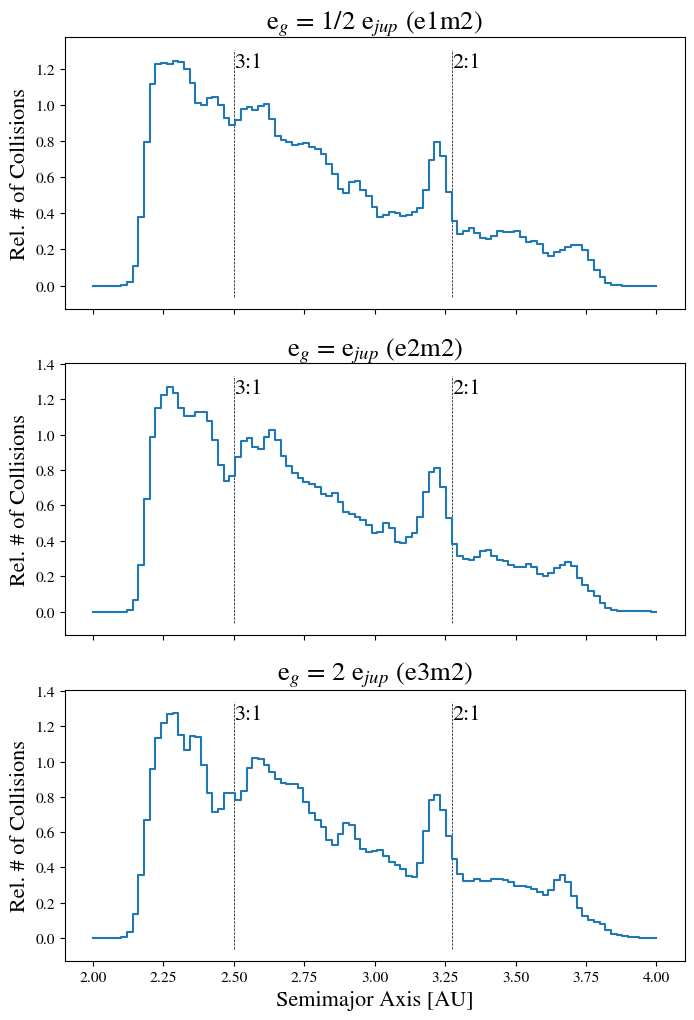
\includegraphics[width=0.5\textwidth]{figures/grind/coll_hist_a.png}
    \caption{A PDF of the collision rate in each disc as a function of semimajor axis, generated using a KDE with a Gaussian 
    kernel with a FWHM of 0.02 au. In semimajor axis space, prominent features appear near the 3:1 and 2:1 MMRs. Near the 
    3:1, the collision rate exhibits a local minimum, while an enhancement appears near the 2:1.\label{fig:coll_hist_a}}
\end{center}
\end{figure}

\begin{figure*}
\begin{center}
    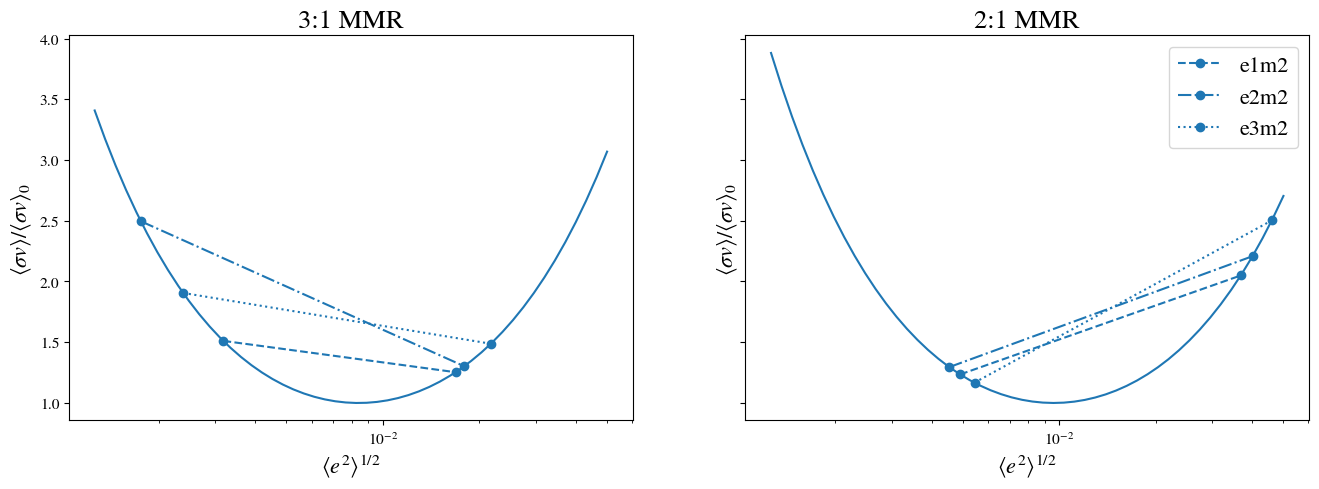
\includegraphics[width=\textwidth]{figures/grind/gf_plot.png}
    \caption{The collision rate (given by equation \ref{eq:saf}) of bodies in the vicinity of the 3:1 (left) and 2:1 (right) MMRs, 
    relative to the minimum value, as a function of the local eccentricity dispersion. The pairs of points connected by lines show 
    the values of the unperturbed (left-hand points in each subplot) and perturbed (right-hand points in each subplot) collision 
    rates in the e1m2, e2m2 and e3m2 simulations. The unperturbed collision rate, along with the amount of dynamical heating 
    that the planetesimal population experiences determines whether the MMR acts to suppress or enhance the collision rate 
    \label{fig:gf}}
\end{center}
\end{figure*}

\begin{figure}
\begin{center}
    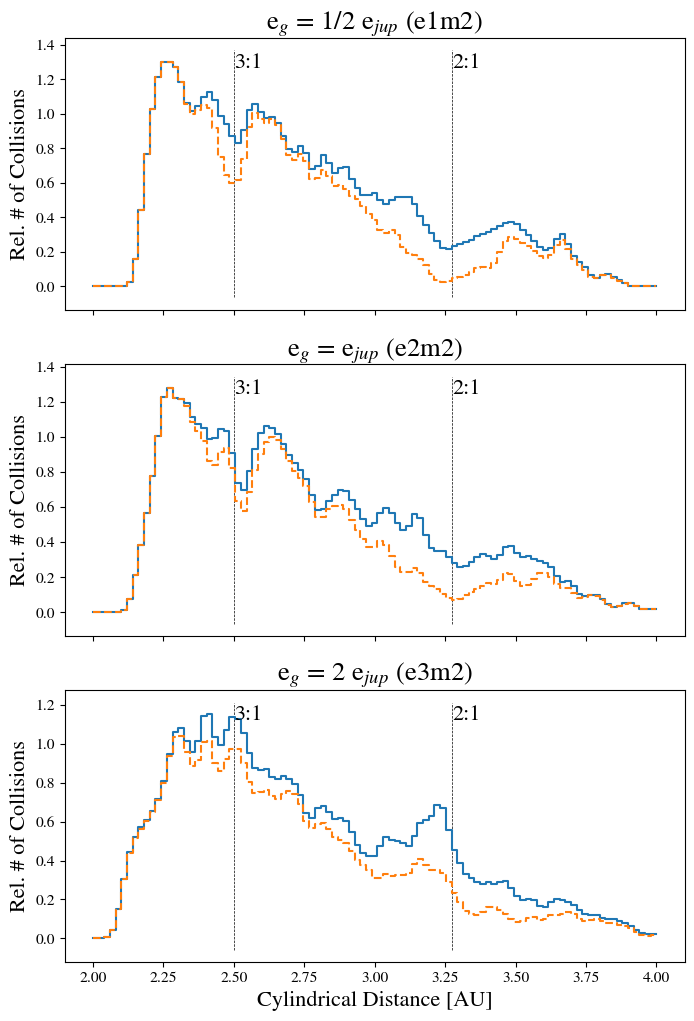
\includegraphics[width=0.5\textwidth]{figures/grind/coll_hist_r.png}
    \caption{Here, collisions are instead ordered by cylindrical distance from the star. Features near the 3:1 and 2:1 MMRs are still 
    present, but appear qualitatively different than in semimajor axis space. At low eccentricities, a dip appears around the center 
    of the resonance. At the highest eccentricity, a bump is formed instead. The dashed lines shown the collision profile with 
    collisions between bodies in resonance removed. The bump and dip features remain qualitatively the same, which suggests 
    that they are produced by bodies outside of the libration width of the resonance.\label{fig:coll_hist_r}}
\end{center}
\end{figure}

\section{Where Does the Dust End Up?}\label{sec:dust}

To construct a radial dust profile from the collision statistics, we begin by making two assumptions: (1) any dust generated by 
collisions is strongly coupled to the gas and (2) any subsequent spatial evolution of the collisional debris is insignificant. So long 
as both of these assumptions are true, we can use the radial locations of planetesimal collisions in the plane of the disk to 
generate a dust profile for each simulation.

We first provide a justification for assumption (1), which is as follows: At 3 au in the protosolar nebula, the mean free path of a 
gas particle is $\sim$ 50 cm (assuming a composition of pure hydrogen with a local volume density of $\rho_{g} = 3 \times 
10^{-11}$ g cm$^{-3}$). This places any dust grains in the Epstein drag regime, with a stopping timescale given by

\begin{equation}\label{eq:ts_epstein}
    t_{s} = \frac{\rho s}{\rho_{g} v_{th}},
\end{equation}

\noindent where $\rho$ is the bulk density of the dust grain, $s$ is its size, and $v_{th}$ is the local thermal velocity of the gas. 
At 3 au in the protosolar nebula, $v_{th} \sim 10^{5}$ cm s$^{-1}$. Assuming a 1 mm dust grain with a $\rho$ = 2 g cm$^{-3}$, 
the stopping time is $\sim 10^{-4}$ yr.  This is orders of magnitude smaller than the orbital timescale; therefore, we conclude that 
collisionally generated dust grains will immediately couple to the gas.

Assumption (2) is less straightforward to justify and may not be reasonable in all cases. Although the spatial redistribution of the 
full-sized planetesimals and mm-sized dust grains is insignificant, the radial drift forces experienced by intermediate-sized bodies 
is much greater. Collisions between planetesimals do not immediately convert the mass to dust grains. Rather, the debris will 
undergo a collisional cascade process, which gradually grinds the resulting bodies down to smaller sizes. A proper treatment of 
the collisional cascade process is quite complicated and is well beyond the scope of this work. However, one may be able to 
ignore this process if the peak radial drift timescale is longer than the timescale for collisions between these bodies.

This occurs for bodies of the size at which $t_{s} \Omega$ = 1. In the Stokes drag regime at 3 au, this occurs for bodies of 1 
meter in size. Following a similar calculation in \ref{sec:pl_drag} with a 1 m body, we find that an object of this size will drift 
across the 2:1 MMR on a timescale of $\sim$ 300 years. Although we do not model collisions between bodies of this size, a 
lower limit on the collision timescale for these objects can be obtained by extrapolating the planetesimal collision rate measured 
in our simulations down. For the e2m2 simulation, we find that 125 collisions occur within the libration width of the 2:1 MMR from 
T=2,000 yr to  T=5,000 yr. There are a total of 15,000 planetesimals within this region, which means that a single planetesimal 
undergoes a collision every $\sim$ 370,000 years on average. If the entire planetesimal population in this region were converted 
to 1 meter bodies with the same bulk density, the number density of bodies increases by a factor of $10^{15}$, while the 
geometric collision cross section decreases by a factor of $10^{10}$. The collision timescale would therefore decrease to $\sim$ 
1 year, which is 2 orders of magnitude smaller than the drift timescale. As shown above, radial drift in the Stokes drag regime is 
maximized for bodies of 1 meter in size, which is only a factor of two larger than the mean free path of the gas particles. It is 
therefore not entirely clear if the Stokes drag law is appropriate here. Because of this, we also repeat the above calculation for 
bodies that experience Epstein drag. With this assumption, we find that radial drift is maximized for a cm-sized body and both 
the radial drift and collision timescale for bodies of that size decrease by a factor of 10 relative to the Stokes values. In both 
cases, collisions between maximally drifting bodies occur on a timescale two orders of magnitude shorter than the drift 
timescale. We therefore argue that it is reasonable and, indeed, best practice to start with such simple assumptions understand 
the physics before additional complexity is later added. We caution, however, that the collision timescale estimates provided 
here should be interpreted as lower limits.

Operating under these assumptions \footnote{As discussed in \cite{boley17}, the local generation of second-generation dust is 
only one consideration. The dust will also evolve spatially due to drag effects, but can also evolve in size or be re-accreted onto 
planetesimals. For simplicity, we focus on local dust sourcing only while acknowledging that subsequent evolution could 
\textbf{also} affect the morphology.}, a map of the relative concentration of second-generation dust can be constructed from the 
cylindrical distance at which the collisions occur. Here, cylindrical distance is defined as the separation between the central star 
and the location of collision in the ($r, \theta$) plane. This is shown in figure \ref{fig:coll_hist_r}. Similar to figure 
\ref{fig:coll_hist_a}, we use a KDE with a width of 0.02 au to assemble the collision locations into a radial distribution. Most 
strikingly, the bump that was present near the 2:1 resonance is no longer visible in cylindrical distance space, although it 
suddenly appears again in the e3m2 simulation. The local minimum that is visible near the 3:1 MMR also becomes a local 
maximum in the highest eccentricity case. To determine how the resonant bodies actually contribute to the radial collision profile, 
we excluded collisions that fall between $2.495 < a < 2.505$ au (near the 3:1 resonance) and between $3.2 < a < 3.35$ au (near 
the 2:1 resonance), which is shown by the dashed curve. As in figure \ref{fig:coll_hist_a}, the solid curves are normalized such 
that the area underneath is equal to 1. For the dashed curves, the normalization factor is scaled according to the number of 
collisions in the entire sample, compared to the number of collisions in the subsample, which excludes the collisions in 
resonance. Qualitatively, none of the bump or dip features present are removed by making this exclusion. This suggests that the 
features near resonance seen in semimajor axis space become smeared out in cylindrical distance space due to the large 
spread in eccentricity and orbital orientation.

This also suggests that the prominent bumps and dips seen in figure \ref{fig:coll_hist_r} are mainly produced by bodies outside 
of the libration width of the resonance, although the resonant population does make some of the features more pronounced. To 
further understand this, we consider the nonaxisymmetric structure seen in figure \ref{fig:xy}. In figure \ref{fig:coll_polar_e}, we 
compare the radial collision profiles to the radial structure seen in the e1m2, e2m2 and e3m2 simulations. In the lowest forced 
eccentricity case (e1m2), the pileups near the edge of the 2:1 MMR line up with the boundaries of the dip feature seen in the 
radial collision profile. The locations of the edges of the resonances are calculated using equations \ref{eq:res_fo} and 
\ref{eq:res_so}. The pileups not as pronounced near the other resonances. As discussed previously, the planetesimal density 
enhancements and gaps seen in polar coordinates follow the position of the giant planet in its orbit, which is shown by the 
vertical line. For the e2m2 case, the density enhancements take up a much larger radial width, which smears out the 
corresponding collisional dust profile. In the highest forced eccentricity case (e3m2), the density enhancements occur well within 
an annulus containing the resonant region, completely altering the radial peak-valley dust morphology.

Although the nonaxisymmetric pileup of bodies near the edges of resonances has been seen previously 

\cite{richardson00, tabeshian16}, we could not find a satisfactory explanation for why it happens, which we will try to provide 
here. As mentioned in section \ref{sec:dynamics}, the circulation frequency of the critical angle slows as one approaches the 
edge of the resonance from the outside. Following the pendulum analogy, this is equivalent toapproaching the point where the 
pendulum becomes suspended in theat top dead center. When the critical angle stays relatively stationary during an encounter, 
the net torque will drive the longitude of pericenter towards the point of conjunction \cite{peale76}.  This is the basic mechanism 
that causes isolated resonances to be stable. Inside of resonance, the critical angle librates about an equilibrium value and this 
configuration is maintained. Just outside of resonance, however, the critical angle slowly drifts away, with the drift direction 
changing sign across the location of exact resonance. The net result of this is that bodies just outside of the resonance 
experience a torque from the planet that temporarily drives their pericenters toward the current orbital position of the planet. After 
the encounter ends, differential rotation of the disc slowly undoes the configuration. As the planet again passes by, adjacent 
planetesimals near the resonance edges temporarily align themselves in this configuration. This explains why the concentration 
of planetesimals appears to `follow' the planet. Connecting this back to the radial collision profiles shown in figure 
\ref{fig:coll_hist_r}, these bodies at the edges of the resonances must be responsible for the bumps and dips morphology seen 
because excluding collisions between bodies inside of the MMRs does not qualitatively alter the profiles.

\begin{figure*}
    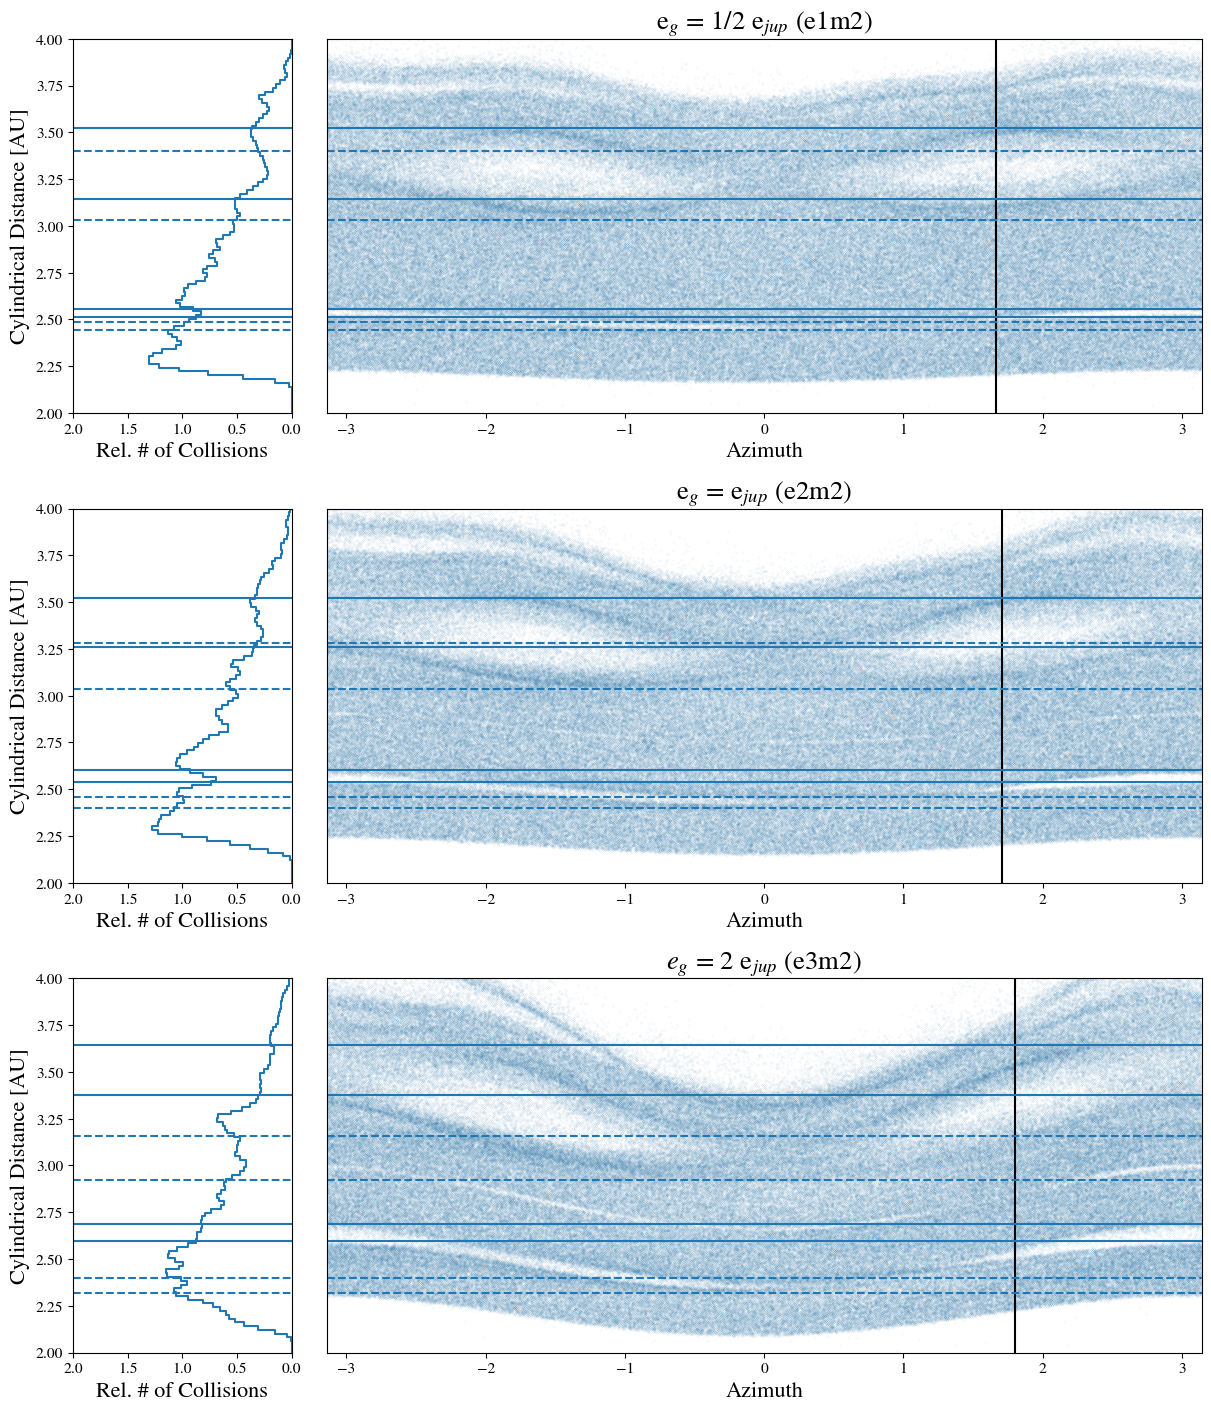
\includegraphics[width=\textwidth]{figures/grind/coll_polar_e.png}
    \caption{The collision profiles in figure \ref{fig:coll_hist_r} are shown alongside the positions of the planetesimals, in polar 
    coordinates. The dashed and solid lines show the pericenter and apocenter, respectively,  of bodies at each edge of the 3:1 
    and 2:1 MMR. In these figures, the longitude of pericenter of the planet lies at $\theta = 0$ and the present position of the 
    planet is indicated by the vertical line. For the 2:1 resonance, a bump, rather than a dip feature appears when the inner edge 
    or the resonance's apocenter and outer edge's pericenter distance cross. The collision profile near the 3:1 resonance does not 
    appear to follow this same qualitative behavior.\label{fig:coll_polar_e}}
\end{figure*}

\begin{figure*}
    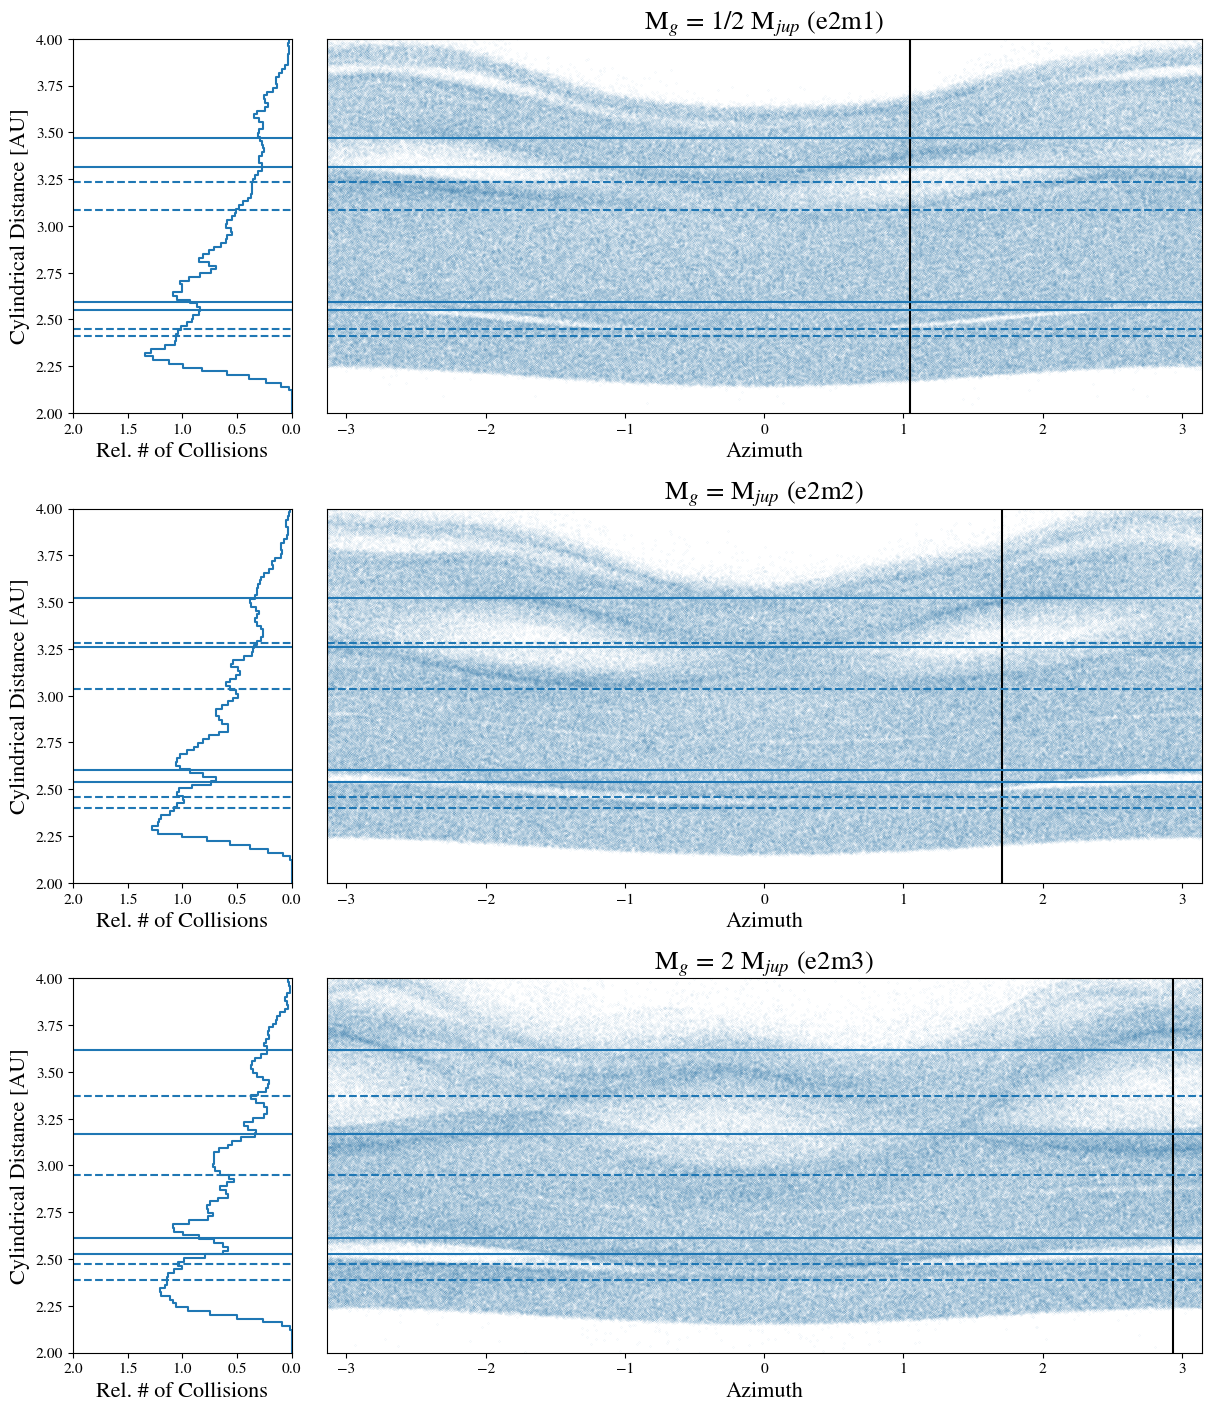
\includegraphics[width=\textwidth]{figures/grind/coll_polar_m.png}
    \caption{Similar to figure \ref{fig:coll_polar_e}, except the eccentricity of the planet is kept constant and the mass is varied.
    This has the effect of changing the width of the resonances, without altering the relative apo or peri distances of bodies near 
    the edges. Except for the highest mass case, the apocenter and pericenter distances of the inner and outer edges of the 2:1 
    resonance are too close together to produce much of a dip or a bump feature.\label{fig:coll_polar_m}}
\end{figure*}

\cite{tabeshian16} provide a different explanation for this phenomenon, suggesting that the nonaxisymmetric structure is the 
product of the path that a resonant test particle takes in a frame co-rotating with the planet (see figure 8.4 of \cite{murray99}). In 
other words, the gap structure is argued to be due to the interfaces between the low eccentricity, non-resonant and high 
eccentricity, resonant regions of the disc. This explanation, however, does not hold for a large collection of planetesimals, 
especially when there is no forced eccentricity. In such a case, the orbits of planetesimals near resonance would be randomly 
aligned, and the axisymmetric structure should become washed out. Furthermore, when the perturbing planet is on a circular 
orbit, this structure is still present (see figure 3 of \cite{tabeshian16} and Appendix \ref{sec:boley_plot}). The only connection 
between the structure of the gaps in the disc and the path of a resonant particle in the corotating frame is that both phenomena 
produce the same symmetries, which depend on the particular MMR considered.

With no secular forcing, this dynamical phenomena should produce an underdensity in the radial surface density profile near the 
center of the resonance and an overdensity at each edge in cylindrical distance space. When a forced eccentricity is introduced, 
the radial location of the resonance edges vary over the course of an orbit. The maximum and minimum radial distance that the 
resonance edges occupy is indicated by the solid and dashed lines in figure \ref{fig:coll_polar_e}. If the the aphelion distance of 
the inner edge becomes close to the perihelion distance of the outer edge, the overdense regions on each side of the resonance 
meet and we should expect to see the central dip feature in the collision profile disappear. This is exactly what appears to be 
happening in the middle panel of figure \ref{fig:coll_polar_e}. As the forced eccentricity is increased further, a region forms at the 
center of the resonance where planetesimals on both sides of the resonance spend time (although not simultaneously). When 
this occurs, a bump feature forms in the collision profile near the center of the resonance. This is apparent in the bottom panel of 
figure \ref{fig:coll_polar_e}.

Although the same phenomenon appears to be happening near the 3:1 MMR, the pileups at the edges of the resonance are not 
as well defined. We attribute this to the more complex symmetry, compared to the 2:1 MMR. In addition, a number of other 
nearby resonances, including the 7:2 (at 2.25 au), the 10:3 (at 2.33 au), the 8:3 (at 2.71 au) and the 5:2 (at 2.82 au) also likely 
are contributing to the collision profile in cylindrical distance space near the 3:1 MMR. The 3:1 MMR is also much narrower than 
the 2:1, which means that any dip or bump features produced by it would require much higher resolution observations. For these 
reasons, we will focus on the 2:1 MMR as the main diagnostic indicator.

\subsection{Varying the Mass}

The dynamical effects of varying the mass of the planet are somewhat simpler, in that doing so does not affect the forced 
eccentricity of the planetesimal disc. Instead, only the width of the resonances changes. The width of a first order resonance 
scales with $m$ (see equation \ref{eq:res_so}), while the leading order terms in the resonant part of the disturbing function, 
which set the strength of the resonance, also scale as $m$. For the 2:1 MMR, the dynamics near the resonance are equally 
sensitive to changes in eccentricity and mass.

We show the polar structure of the e2m1, e2m2 and e2m3 simulations in figure \ref{fig:coll_polar_m} alongside the radial 
collision profile. In all three cases, the eccentricity of the perturbing planet is set to $e_{jup}$. Changes in the apocenter and 
pericenter distances of the edges of the resonances are entirely due to changes in the resonance width. For the e2m1 and e2m2 
simulations, the inner apocenter and outer pericenter distances near the 2:1 MMR are quite similar and no strong features 
appear in the collision profile near this region. For the e2m3 case, the edges ofthe resonances are sufficiently separated to allow 
what appears to be the beginning of gap to form near the center of the 2:1 resonance in the collision profile.

\subsection{Observability of the Dust}

While the collisional dust profiles show radial amplitude variations, we still need to assess whether those variations could be 
observable. To proceed, we create a sky model for simulated ALMA observations as follows. First, we use the radially-averaged 
collision profile from each simulation (see figures \ref{fig:coll_polar_e} and \ref{fig:coll_polar_m}) as the template for an 
azimuthally symmetric disc. We then scale the size of each profile by a factor of ten, which places the perturbing planet at 52 au. 
This scaling is permitted by the dynamics (both the resonance widths and the forced eccentricities are scale-free) and makes the 
disc comparable in size to the many discs that have now been observed by ALMA \cite{huang18}. The angular size scale is then 
set by envisaging a face-on disc at a distance of 100 pc.  

The sky model intensity (flux per pixel) is produced by interpolating the radial collision frequency onto a 2D Cartesian grid with 
cell widths of approximately 2 mas. In doing so, we choose to make the intensity proportional to the collision frequency (i.e., the 
dust) because it is the most straightforward case. Many different parameterizations are possible, depending on optical depth, 
grain size, disc temperature, etc., but we will avoid such complications here, as they would affect the overall brightness profile, 
but not the presence of any gaps or rings. We normalize the intensity bysetting the total disc flux density to be 100 mJy at about 
350 GHz.  

The simulated observations are performed using the {\sc simobserve} task in {\sc CASA} \cite{mcmullin07}.  The disc is given an 
$\rm RA = 11^{\rm h} 01^{\rm m} 52^{\rm s}$ and a $\delta = -34^\circ 42\arcmin 17\arcsec$ (i.e., the J2000 coordinates for TW 
Hydrae) and is ``observed'' through transit on March 20, 2020. We observe the disc using configurations 8, 9, and 10 at 350 GHz 
(cycle 6 antenna file), spending six hours on-source in each configuration\footnote{We have imagined that the TAC really likes 
us.}.  The visibilities are corrupted with thermal noise, setting the precipitable water vapor to 1.5 mm. They are then combined, 
imaged, and cleaned using the task {\tt tclean}. Imaging uses Briggs weighting with a robustness parameter of -1. 

The results for the nominal simulation (e2m2) are shown in figure \ref{fig:alma_sim_obs}. The 3:1 and 2:1 resonances can be 
easily identified in the cleaned image and in the corresponding radial profile.  Moreover, the features are qualitatively similar to 
the bright rings and dark gaps seen in actual disc profiles \cite{alma15}.

In figure \ref{fig:alma_profiles}, we show the azumithally-averaged radial profiles constructed from the simulated cleaned image 
from all five simulations. In all cases, a bump or a dip feature is clearly visible at the location of the 3:1 and 2:1 MMRs, indicated 
by the dashed vertical lines. As mentioned previously, the feature at the 2:1 MMR acts as the actual diagnostic indicator, while 
the 3:1 resonance (along with the gap that would presumably open at the location of the planet) is mainly useful for determining 
where the 2:1 MMR is actually located.

\begin{figure}
\begin{center}
    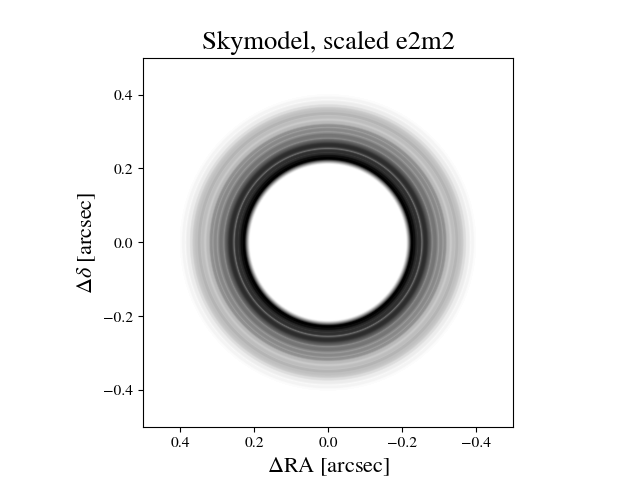
\includegraphics[width=0.5\textwidth]{figures/grind/skymodel_e2m2.png}
    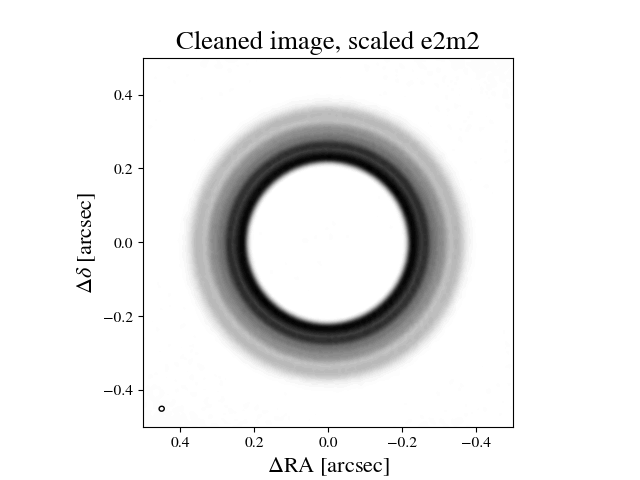
\includegraphics[width=0.5\textwidth]{figures/grind/xy_e2m2.png}
    \caption{Simulated ALMA observations for the nominal (e2m2) case, operating under the assumption that the dust profile 
    closely traces the planetesimal collision profile.  Top: The sky model based on the radial collision distribution. The size of the 
    disc has been scaled by a factor of 10 and placed at  a distance of 100 pc. Bottom: The cleaned image using combined 
    observations in configurations 8, 9, and 10. The circle in the bottom left indicates the simulated beam size. Gaps in the dust 
    due to the 3:1 and 2:1 resonances are visible. 
    \label{fig:alma_sim_obs}}
\end{center}
\end{figure}

\begin{figure*}
    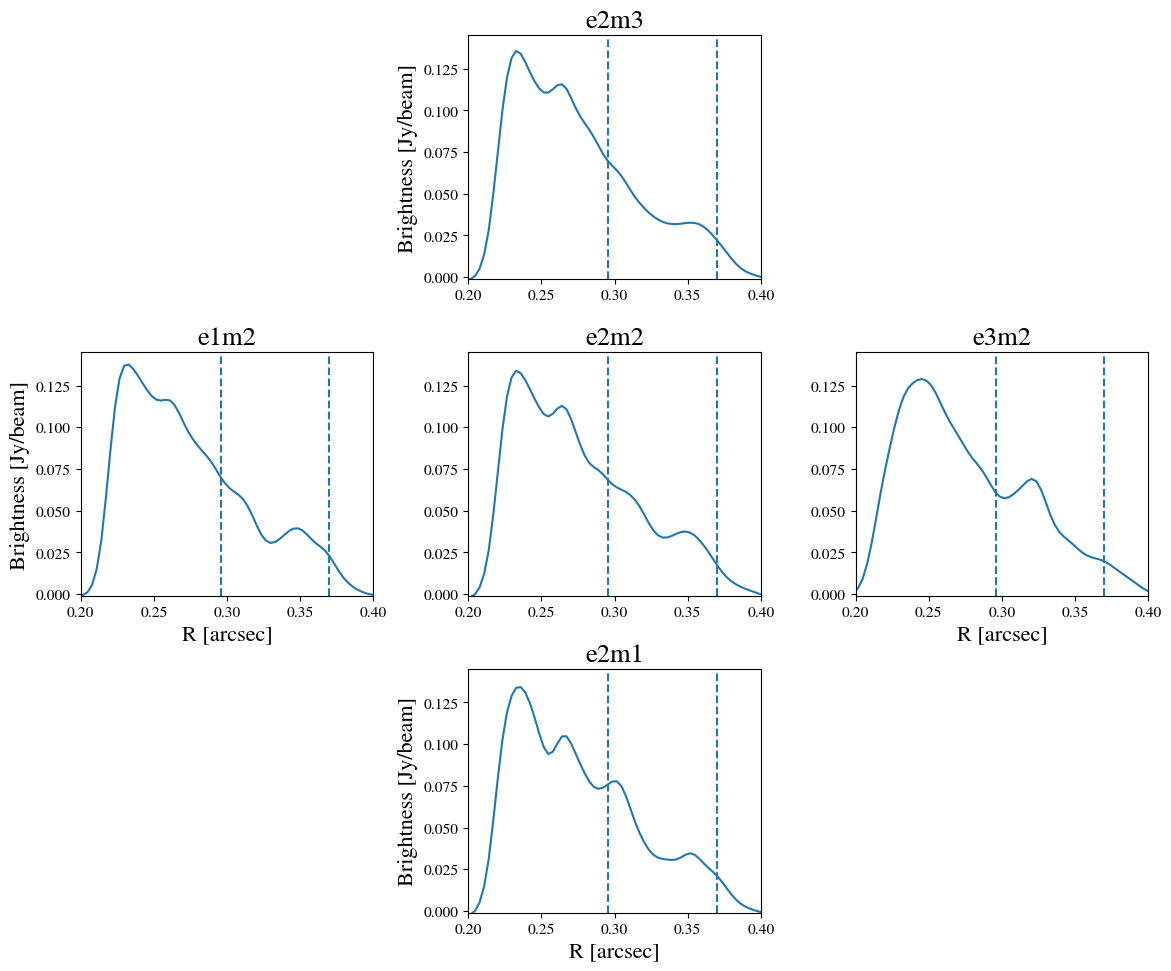
\includegraphics[width=\textwidth]{figures/grind/alma_profiles.png}
    \caption{The azimuthally-averaged radial profile based on the simulated cleaned images from all five simulations. The 
    eccentricity of the perturbing planet increases from left to right, while the mass of the planet increases from bottom to top. The 
    vertical dashed lines indicate the locations of the 3:1 and 2:1 resonances. As in figure \ref{fig:alma_sim_obs}, the size scale of 
    the disc has been expanded by a factor of 10 and then placed at a distance of 100 pc.\label{fig:alma_profiles}}
\end{figure*}

\section{Constraining the Mass and Eccentricity of the Planet}\label{sec:constrain}

\begin{figure}
\begin{center}
    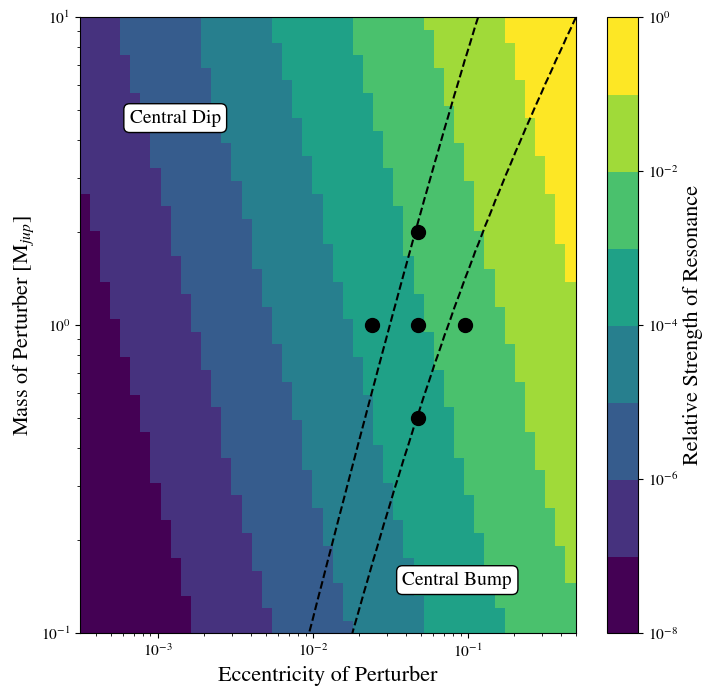
\includegraphics[width=0.5\textwidth]{figures/grind/bump_dip_diag.png}
    \caption{The presence of a dip or bump in the collision profile (and therefore the dust profile) near the 2:1 MMR can be used 
    to constrain the mass and eccentricity of the perturbing planet. The color scale indicates the relative strength of the features, 
    while the dashed lines indicate boundaries in parameter space where a dip or a bump will be produced at the resonance. 
    Combinations of mass and eccentricity that fall between the dashed lines correspond to an inner apocenter and outer 
    pericenter separation at the edges of the resonance that is smaller than the resonance width and therefore will not create any 
    significant feature in the collision profile.\label{fig:bump_dip_diag}}
\end{center}
\end{figure}

The simple bump vs dip structure that we expect to reveal itself in the dust emission from colliding planetesimals in near-
resonance with a giant planet could potentially be used to place constraints on the mass and eccentricity of the planet. Near the 
2:1 MMR, the central dip feature is only produced when bodies at the edges of the resonance stay sufficiently separated in 
cylindrical distance over the course of an orbit. This is achieved when either the resonance width is large or the forced 
eccentricity is small. The bump feature, on the other hand, is produced when there is a sufficiently large amount of overlap 
between the apocenters and pericenters of the inner and outer edges of the resonance, respectively. This is achieved when the 
resonance is narrow and the forced eccentricity is large.

In figure \ref{fig:bump_dip_diag}, we show the constraints that the presence of a bump or a dip or dip at the 2:1 MMR places on 
possible values of $(m_{g}, e_{g})$. The dashedlines indicate regions of parameter space where qualitatively different features in 
the collision profile are expected to form. Above the upper dashed line, the resonance is wide while the radial excursion distance 
of planetesimals at the edge of the resonance is small, which gives rise to a dip in the collision profile. Below the lower dashed 
line, the resonance is narrow, while the radial excursion distance is large, allowing the apocenter and pericenter distances of the 
edges of the resonance to overlap and produce a bump in the collision profile. Between the dashed lines, the absolute value of 
separation between the apocenter and pericenter distances of the inner and outer edges of the resonance is less than the 
resonance width. In this region of parameter space, no significant features in the collision profile near the 2:1 MMR are expected 
to form. 

Because the strength\footnote{More specifically, the strength of the resonant term in the disturbing potential} of the 2:1 
resonance scales with $e_{g}$ and  $m_{g}$, a sufficiently low mass and low eccentricity planet will not create enough of a 
perturbation in the planetesimal disc to produce a detectable bump or dip feature. The colored contours in figure 
\ref{fig:bump_dip_diag} indicate the relative strength of the resonance as these quantities are varied. Although the resonance 
strength is equally sensitive to changes in mass and eccentricity, the peri-apocenter overlap of the resonance edges is more 
sensitive to changes in eccentricity. This is because changes to eccentricity affect both the resonance width and the forced 
eccentricity. As we showed in figure \ref{fig:coll_polar_m}, changing $m_{g}$ by a factor of 4 produced very minimal changes to 
the resulting dust profile.

In order to actually identify the 2:1 MMR in the dust emission, at least one other resonance must be visible. Assuming the 
gravitational field in the disc is near-Keplerian, the distance ratios between two features can be used to determine period ratios, 
which can be used to confirm whether the features seen are indeed resonances. Although the 3:1 MMR does not appear to 
follow the simple bump vs dip dichotomy described above, its presence should be marginally detectable in all of the cases 
shown above.

We would again like to emphasize that the dust emission profiles in figure \ref{fig:alma_profiles} are constructed upon the 
assumption that the radial dust structure closely traces the collision profile of the planetesimals. For this assumption to be valid, 
the resulting dust must remain locally confined, which can be achieved if the grains are reaccreted onto planetesimals 
\cite{johansen15}. It is also necessary that the collisional cascade from which the dust grains form plays before radial drift has a 
chance to move debris away from the resonances. Although we showed with a back-of-the-envelope calculation (see section 
\ref{sec:dust}) that this is plausible for a typical protoplanetary disk with properties similar to the protosolar nebula, a more 
thorough treatment of collisional grinding and the subsequent evolution of the debris is necessary to be able to interpret the dust 
emission profiles presented here as anything more than upper limits.

\section{Summary and Conclusions}\label{sec:conclusions}

In this work, we have shown that mean-motion resonances with a perturbing planet produce significant local variations in the 
collision rate of a planetesimal disc. In contrast to \cite{richardson00}, we find that the more prominent interior MMRs, including 
the 2:1, 3:1 and 5:3, all produce structure in the collision profile as a function of semimajor axis. Furthermore, we find that a 
series of distinctly different features appear when collisions are ordered by cylindrical distance from the central star. The 
morphology of these features are tied to dynamical behavior of bodies near the edges of the resonances, where the circulation 
frequency of the critical angle approaches infinity. Particularly near the 2:1 MMR, we find that a bump or dip in the collision 
profile forms when collisions are ordered by cylindrical distance. The presence of one of these two features depends on the peri- 
and apocenter distances of the edges of the resonance, relative to the libration width. Because these quantities depend on the 
mass and eccentricity of the perturbing planet, these properties of the planet are actually encoded in the collision profile.

Near the interior 2:1 MMR, we find that a distinct bump or dip feature is generated in the collision profile, depending on the 
properties of the perturbing planet. The presence of one of these two structures can used to constrain the mass and eccentricity 
of the planet. For a high mass, low eccentricity planet, a dip will form because the edges of the resonance, where many 
collisions occur, stay sufficiently separated. If the planet has a low enough mass (which shrinks the size of the resonance) or is 
sufficiently eccentric (which decreases the separation between the apocenter and pericenter distances of the edges of the 
resonance), a bump will instead form. We tested this hypothesis for five different combinations of the planet's mass and 
eccentricity and found that a distinct bump or dip signature is produced as long as the planet properties are sufficiently far from 
the dividing line in parameter space. This diagnostic is more useful for massive, eccentric planets, because the strength of the 
resonant perturbations scale linearly with both of these quantities.

Although the planetesimal collision profile would not be directly observable in a planet-forming disc, the dust from the resulting 
collisional cascade could potentially be used to trace it. So long as the dust grains are well-coupled to the gas and radial drift 
does not have a significant effect on the morphology of the dust, the bump or dip features seen in the collision profile will also 
appear in the dust profile. Assuming that this is the case, we have generated simulated observations of a protoplanetary disk 
with ALMA and showed that the bump or dip features seen in the collision profiles should be detectable through the dust 
emission. From a dust emission profile with sufficiently strong radial features, one could constrain the properties of a perturbing 
planet on an exterior orbit in the following way: (1) identify the locations of two MMRs in the disc (2) measure the spacing 
between them to verify that one of the features is indeed associated with the 2:1 MMR (3) determine whether an under- or 
overdensity in the radial dust profile exists near this location (4) use the presence of one of these two features to determine the 
region of the eccentricity-mass plane in which the planet lies.

In line with \cite{boley17}, the results of this work suggest that, in planet forming discs, the observed dust structure should not be 
interpreted as simply the result of primordial dust that is perturbed by the planets and gas. Instead, some morphological features 
could be the product of collisional dynamics between larger bodies. Within the confines of the simulations presented here, we 
have shown that this second-generation dust can give rise to significant features in the dust emission profile. For this reason, we 
emphasize that planet-forming discs should be thought of as existing along an evolutionary continuum, with the youngest discs 
being dominated by primordial dust and gas and the most evolved discs being comprised of mainly collisionally generated dust.

The results presented here appear to be broadly consistent with the planetesimal dynamics seen by \cite{tabeshian16}. In their 
case, a dip feature can be seen in the azimuthally averaged surface density profile, although they did not test a high enough 
eccentricity planet in any of their simulations to produce a bump. Another thing to note is that the gap morphology seen by 
\cite{tabeshian16} was markedly different for the 2:1 exterior MMR. Whether this would alter the radial collision profile for the 
exterior, rather than the interior 2:1 resonance, is not immediately clear.  On one hand, the solid surface density diminishes with 
distance ($\sim r^{-3/2}$ for the MMSN \cite{hayashi81}), which would weaken the signal from locally generated collisional dust. 
On the other hand, exterior MMRs are quite effective at capturing inward drifting bodies \cite{weidenschilling85}, which could 
locally enhance the surface density well beyond the MMSN value. A full treatment of the collisional cascade process and the 
radial drift of debris is a subject that we leave for future work.

Compared to using the corotating gap opened by the planet as a diagnostic \cite{dobinson13, dobinson16}, measuring variations 
in the dust emission near MMRs is much more subtle and requires much higher spatial resolution and sensitivity. As we have 
shown, the bump vs dip feature near the 2:1 MMR is marginally detectable with ALMA for the nearest protoplanetary discs, so 
long as the dust profile closely matches the collisional profile of the planetesimals. Another complicating factor is that the inner $
\sim$ 10 au of most protoplanetary discs are optically thick in the sub-mm. The solution to this problem is to instead observe at 
longer wavelengths where the inner disc is optically thin. This comes at the expense of much poorer resolution. However, future 
radio facilities like the NG-VLA are expected to achieve sub-au resolution for nearby planet-forming discs \cite{ricci20}. In the 
more near-term, techniques like Gaussian process fitting present a promising way to recover substructure at sub-beam 
resolution \cite{jennings20}.

\section{Appendix A: Timescale for Secular Forcing}\label{sec:sec_forcing_timescale}

The timescale for secular forcing is given by the period at which the free eccentricity of a body cycles in the complex plane. The 
time-dependent imaginary and real components of the eccentricity of a planetesimal are given by \cite{murray99} (see ch. 7, pg. 
282, eq. 7.51)

\begin{eqnarray}\label{eq:kandh}
	h = e_{1} sin (g_{1} t + \beta_{1}) + e_{2} sin (g_{2} t + \beta_{2}) \\ \nonumber
	k = e_{1} cos (g_{1} t + \beta_{1}) + e_{2} cos (g_{2} t + \beta_{2}),
\end{eqnarray}

\noindent where  ($e_{1}$, $e_{2}$) and ($g_{1}$ , $g_{2}$) are the corresponding eigenvector components and eigenvalues of 
a matrix, which describes the secular interaction between two bodies, given by \cite{murray99} (see ch. 7, pg. 276, eq. 7.9 and 
7.10, with $\alpha_{12} = \alpha$ and $\bar{\alpha_{12}} = 1$)

\begin{eqnarray}\label{eq:pert_matrix}
	A_{jj} = n_{j} \frac{1}{4} \frac{m_{k}}{m_{c} + m_{j}} \alpha b_{3/2}^{(1)} (\alpha) \\ \nonumber
	A_{jk} = -n_{j} \frac{1}{4} \frac{m_{k}}{m_{c} + m_{j}} \alpha b_{3/2}^{(2)} (\alpha).
\end{eqnarray}

\noindent Here, $n$ is the mean motion of a body and $m$ is its mass. In the case of a massless test particle being perturbed by 
a giant planet, $m_{1} = m_{g}$ and $m_{2} = 0$. The frequency of the secular forcing is simply the difference of the two 
eigenvalue frequencies $g_{1} - g_{2}$.

\section{Appendix B: Libration in Mean Motion Resonance}\label{sec:libration}

For second order and higher MMRs, the maximum libration width is given by \cite{murray99} (ch. 8, pg. 338, eq. 8.58) as

\begin{equation}\label{eq:res_so}
	\frac{\delta a}{a} = \pm \left( \frac{16}{3} \frac{\left| C_{r} \right|}{n} e^{\left| q \right|} \right)^{1/2},
\end{equation}

\noindent where $n$, $a$ and $e$ are the mean motion, semimajor axis and eccentricity of the unperturbed body. $C_{r}$ is a 
constant defined by $m'/m_{c} n \alpha f_{d}(\alpha)$, where $\alpha$ = $a/a'$ and $f_{d}$ is the resonant part of the disturbing 
function. For an interior second-order resonance,

\begin{eqnarray}\label{eq:fd_so}
	f_{d} (\alpha) &=& \frac{1}{8} \left[ -5(p+q) + 4(p+q)^{2} - 2 \alpha D \right. \\ \nonumber
	                      & + & \left. 4(p+q) \alpha D + \alpha^{2} D^{2} \right] b^{p+q}_{1/2},
\end{eqnarray}

\noindent (see \cite{murray99} table 8.1, third row, with $j = p + q$) where $D b^{j}_{s}$ is the first derivative with respect to $
\alpha$ of the Laplace coefficient defined in equation \ref{eq:lap}. This is given by \cite{brouwer61} as

\begin{equation}\label{eq:lap_d}
	\frac{d b_{s}^{j}}{d \alpha} = s \left( b_{s+1}^{j-1} - 2 \alpha b_{s+1}^{j} + b_{s+1}^{j+1} \right).
\end{equation}

For a first-order resonance, the associated disturbing function terms are slightly simpler such that

\begin{equation}\label{eq:fd_fo}
	f_{d}(\alpha) = -(p+q) b_{1/2}^{p+q} - \frac{\alpha}{2} D b_{1/2}^{p+q},
\end{equation}

\noindent (see \cite{murray99} table 8., first row) and there is an additional contribution to the motion of the critical angle by the 
pericenter precession rate such that

\begin{equation}\label{eq:res_fo}
	\frac{\delta a}{a} = \pm \left(\frac{16}{3} \frac{\left| C_{r} \right|}{n} e \right)^{1/2} \left(  1 + \frac{1}{27 p^2 e^3} \frac{\left| C_{r} \right|}{n} 
	\right)^{1/2} - \frac{2}{9 p e}  \frac{\left| C_{r} \right|}{n}
\end{equation}

\noindent (see \cite{murray99} ch. 8, pg. 340, eq. 8.76, with $j_{2} = p$).

In mean-motion resonance, the orbital elements of a perturbed body, along with the critical angle described by equation
\ref{eq:phi_crit}, will exhibit oscillations. In the circular, restricted three-body case, these small amplitude oscillations exhibit a 
characteristic frequency, given by (see \cite{murray99} ch. 8, pg. 332, eq. 8.47, with $j_{2} =-p$ and $j_{4} = -q$)

\begin{equation}\label{eq:lib_time}
	\omega_{0} = 3 p^{2} C_{r} n e^{\left| -q \right|}.
\end{equation}

\section{Appendix C: Nonaxisymmetric Structure in Boley 2017}\label{sec:boley_plot}

\begin{figure*}
    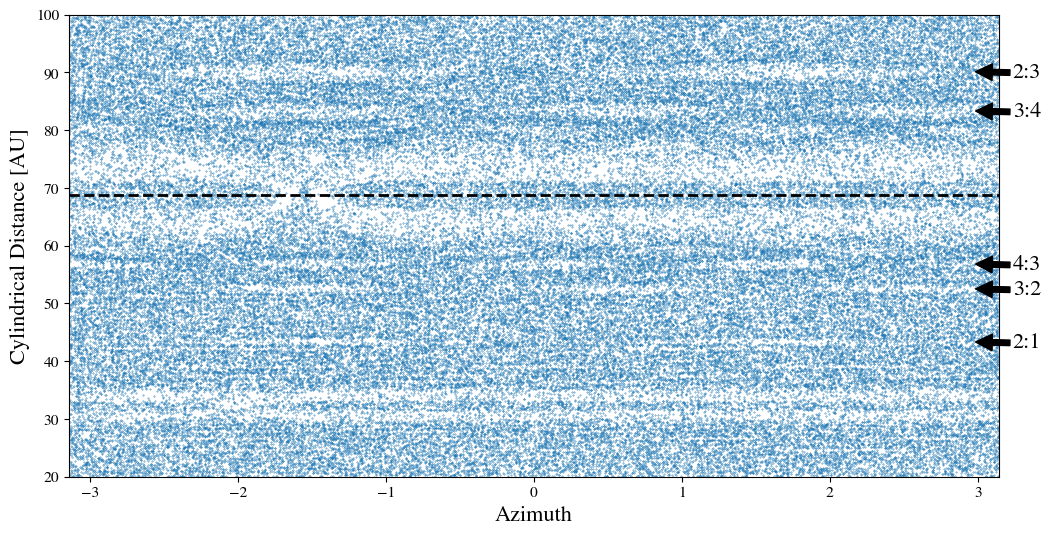
\includegraphics[width=\textwidth]{figures/grind/boley_rtheta.png}
    \caption{Positions of planetesimals at the end of the simulation presented in \cite{boley17} in polar coordinates. The dashed 
    line marks the location of a 50 $M_{\earth}$ planet embedded in the disc. First order MMRs with the planet are indicated with 
    arrows. A second planet is also present at 32.3 au, although it is not massive enough to induce any significant structure in the 
    disc near associated resonances.\label{fig:boley_rtheta}}
\end{figure*}

As mentioned in section \ref{sec:vary_ecc}, the nonaxisymmetric gap structure seen in figure \ref{fig:xy} is present in a number 
of other studies, including \cite{richardson00} and \cite{tabeshian16}. One would expect the same dynamics to be at work in the 
simulation of \cite{boley17}, although the structure is not obviously visible in figure 3 of their work.

Here, we present a closer look at the positions of the planetesimals at the end of the \cite{boley17} simulation. In figure 
\ref{fig:boley_rtheta}, we show the planetesimal positions in polar, rather than Cartesian coordinates as originally presented in 
the paper. Two planets on circular orbits are present here. The first has mass of 17 $M_{\earth}$ and lies at 32.3 au. The second 
planet has a mass of 50 $M_{\earth}$ and lies at 68.8 au. A horseshoe shaped collection of planetesimals is visible to be 
corotating with each planet. Nonaxisymmetric gaps are alsovisible at the locations of first order MMRs with the more massive 
planet, which are indicated with arrows.

Similar to figure \ref{fig:coll_polar_e}, a gap is present at the same orbital phase as the planet at the 2:1 MMR, along with a 
second gap on the opposite side of the disc. Gaps near the 4:3 and 3:2 MMRs are also present in phase with the planet, 
although the number and spacing between additional gaps appears to be different for each resonance. In addition, the gap 
structure associated with the exterior MMRs appears markedly different than that of each corresponding interior MMR, which 
suggests that the structure is related to the symmetry of the path that a planetesimalin a frame corotating with the planet takes.
\chapter {Formation of Planetary Embryos at Short Orbital Periods}\label{ch:stipPl}

\noindent \textit{The content of this chapter was originally published in collaboration with Thomas R. Quinn in the X XXXX edition of The Astrophysical Journal(\cite{wallace23}, ApJ, Vol. XXX, X; 20XX, DOI: XXXX), and is reproduced below with the permission of the American Astronomical Society.}

\section{Introduction} \label{sec:intro}

Planetesimal accretion is a key phase in the terrestrial planet growth
process, bridging the gap from kilometer-sized bodies up to roughly
moon-sized objects known as planetary embryos. In the earliest stages
of the planet formation process, beginning from $\mu$m sizes, aerodynamic forces dominate the
growth and evolution of the solids and statistical models
\cite{johansen14, birnstiel16} are appropriate to describe how these
numerous, small bodies coagulate. 

Due to the internal pressure support
of the gas disk, the gas itself orbits at sub-Keplerian speed and
exerts a headwind on any solids large enough to decouple from the gas
\cite{weidenschilling77}. Around a meter in size, this headwind
is maximally effective at sapping away orbital angular momentum, and planet-building material can fall onto the central star on 
catastrophically short timescales \cite{weidenschilling77, nakagawa86}. Additionally, laboratory experiments suggest that 
collisions between mm- to cm- sized solids tend to result in bounces or destruction, rather than continued growth
\cite{blum93, colwell03, beitz11}.

For these reasons, a number of mechanisms to radially concentrate solids in a planet-forming disk have been proposed to 
facilitate fast growth from mm to km sizes \cite{johansen07, lyra08, bai10} in order to surmount these barriers. Interestingly, 
formation models for the short-period multiplanet systems revealed by Kepler \cite{fabrycky14} also seem to require enhanced 
concentrations of planet-building material to reproduce the observed architectures \cite{raymond07, hansen12}.

Regardless of how the mm- to km-sized growth barriers are surmounted, gravity begins to dominate and aerodynamic gas drag 
plays an increasingly unimportant role beyond this size. During this phase, collision cross sections are enhanced as gravitational 
focusing \cite{safronov69} acts to bend the trajectories of bodies undergoing close encounters. Because gravitational focusing 
becomes more effective as bodies grow larger, a period of runaway growth occurs \cite{wetherill89, kokubo96, barnes09} and a 
power law spectrum of masses develop. Eventually, the largest bodies (known as oligarchs) dynamically heat the remaining 
planetesimals, severely limiting further growth \cite{kokubo98}. The final outcome of this phase is a bimodal population of 
dynamically cold oligarchs, surrounded by dynamically hot, difficult to accrete residual planetesimals. Lines of evidence suggest 
that the asteroid belt \cite{bottke05, morbidelli09}, Kuiper belt \cite{duncan89, levison08, sheppard10} and the Oort cloud  \cite{levison11} are largely composed of the leftovers of this stage of planet formation.

Tidal interactions between protoplanets and the gaseous disk keep eccentricities and inclinations low until the gas disk dissipates, typically over the course of a few Myr \cite{mamajek09}. Eventually, gravitational perturbations trigger an instability which drives bodies onto crossing orbits. This instability occurs on a timescale of $\sim 10^{5}$ years and involves large scale oscillations of the eccentricity and inclinations of the bodies as they strongly interact through secular resonances \cite{chambers98}.
As a consequence of the instability, the oligarchics are no longer
on isolated, stable orbits and coalesce to form Earth-sized planets
through a series of extremely energetic giant 
impacts \cite{kokubo02, raymond05, raymond06}. 

Due to the relative ease of modeling the early dust coagulation phases
and the final giant impact phase, these steps in the terrestrial
planet formation process have received most of the attention in the
literature. The planetesimal accretion phase, which we will focus on
in this chapter, is more difficult and expensive to model because there are too
many particles to directly track with traditional N-body codes, while
the gravitational interactions between the few massive bodies produced by the runaway growth phase \cite{ida93, kokubo95, kokubo98} render statistical methods inappropriate. Due to computational expense, N-body simulations of
planetesimal accretion are usually modeled in a narrow
ring \cite{kokubo96, kokubo98}, and the results and timescales are then scaled to suit whatever relevant orbital period is being 
studied. N-body simulations of terrestrial planet assembly typically begin with a series of neatly spaced oligarchs, whose mass 
varies smoothly with orbital period. As we will show in this chapter, oligarchic growth does not scale to arbitrarily short
orbital periods.

Given that Systems of Tightly-packed Inner Planets (STIPs) appear to
be a common outcome of planet formation \cite{lantham11, lissauer11, rowe14}, understanding exactly how
solids accumulate at short orbital periods is crucial. Although
gas-disk driven migration of the planets themselves is often invoked
to explain the observed architectures \cite{izidoro17, izidoro21}, we will focus on an in-situ
model in this chapter. That is, once the planetesimals themselves form,
they largely stay in place, and any subsequent large-scale movement of
the solids are the result of mutual gravitational interactions. The
focus of this work will be to understand how the outcome of the
planetesimal accretion process scales with orbital period by using a
high-powered N-body code to directly follow the growth and evolution
of the planetesimals across a wide range of orbital periods (1 to 100
days). In doing so, we will assess whether the typical initial conditions (fully formed, evenly spaced protoplanets, e.g. \cite{raymond06}) used in studies of terrestrial planet formation are actually appropriate for understanding STIPs.

In section \ref{sec:theory} we provide an overview of the theory
behind planetesimal accretion and show that assumptions used to derive
the well-known modes of growth are only valid at sufficiently long
orbital periods. We then motivate the need for N-body simulations to
study this problem and describe the code used, along with how our
initial conditions were constructed in section \ref{sec:methods}. In
section \ref{sec:narrow}, we present a parameter study of planetesimal
accretion using a series of simulations of narrow annuli that exhibit both oligarchic and non-oligarchic growth. In section 
\ref{sec:fulldisk} we present a set of simulations starting with a  wide planetesimal disk and demonstrate that a transition 
between accretion modes occurs at moderately small orbital periods. Next, we assess the impact of 
simplifications made to our collision model on this result in section \ref{sec:assump}. In section \ref{sec:pl_stip_discuss}, we discuss the 
implications of this multimodal accretion behavior throughout the disk for planet formation models and conclude.

\section{Overview of Planetesimal Accretion}\label{sec:theory}

\subsection{Oligarchic and Runaway Growth}

We begin our analysis by considering a disk of equal mass planetesimals
with radius $r_{pl}$, mass $m_{pl}$ and surface density
$\Sigma_{pl}$. The collision rate in the vicinity of an orbit defined
by Keplerian frequency $\Omega$ can be written as $n \Gamma v$, where
$n = \Sigma_{pl} \Omega / 2 m_{pl} v$ (where we have assumed that the scale height of the planetesimal disk goes as $2v/\Omega$). $\Gamma$ describes the effective
collision cross section and $v$ is the typical encounter velocity
between planetesimals.
For a swarm of planetesimals on randomly oriented orbits, $v$ is typically
taken to be the rms velocity, $\left< v^{2} \right>^{1/2}$, which can be related to the eccentricity and inclination distribution $(e, i)$ in the following way \cite{lissauer93}:
\begin{equation}\label{eq:ecc_vel}
	\left< v^{2} \right>^{1/2} = \left( \frac{5}{4} \left< e^{2} \right>^{1/2} + \left< i^{2} \right>^{1/2}  \right) v_{k}.
\end{equation}

The dynamical interactions between growing planetesimals can be somewhat simplified by scaling the orbital elements of the bodies by
the Hill radius

\begin{equation}\label{eq:hillfac}
	r_{h} = \left(\frac{m_{pl}}{3 M_{*}}\right)^{1/3}, 
\end{equation}
\noindent where $M_{*}$ is the mass of the central star. The Hill radius of a body describes the size scale over which the gravity of the growing planetesimal dominates over the gravity of the star. Using equation \ref{eq:hillfac}, the eccentricity, inclination and separation between orbiting bodies can be defined as

\begin{equation}\label{eq:hillorb}
	e_{h} = \frac{a e}{r_{h}}, \: i_{h} = \frac{a i}{r_{h}}, \: \tilde{b} = \frac{a_{2} - a_{1}}{r_{h}}.
\end{equation}

\noindent Using this formalism, $e_{h}$ and $i_{h}$ describe the radial and vertical excursions of an orbiting body in units of its Hill radius. For $e_{h} > 1$, the random velocity dispersion dominates over the shearing motion across a separation of $1 r_{h}$ and encounters can be treated with a two-body formalism.

Assuming that every collision results in a perfect merger, the growth rate of a planetesimal is given by
\begin{equation}\label{eq:growth}
	\frac{1}{M}\frac{dM}{dt} = \frac{\Sigma \Omega}{2 m_{pl}} \Gamma.
\end{equation}
\noindent In the case where the collision cross section depends only
on the physical size of the planetesimals, the growth scales sub-linearly
with mass and the mass distribution is expected to evolve in an
``orderly'' fashion, in which mass ratios between bodies tend toward unity. However, bodies larger than $\sim 100$ km in size are expected to exert a significant gravitational force on each other during encounters and the collision cross section depends on both the size of the bodies and their encounter velocities. In this case, 
\begin{equation}\label{eq:gravfocus}
	\Gamma = \pi r_{pl}^2 \left( 1 + v_{esc}^2 / v^2 \right)
\end{equation}
\cite{safronov69}, where $v_{esc}$ is the escape velocity from the two bodies at the point of contact.

In the limit that $v_{esc} \gg v$, it can be shown that $dM/dt \propto
M^{4/3}$, which implies a runaway scenario where growth
accelerates with mass. This mode of growth was confirmed with N-body
simulations by \cite{kokubo96} and appears necessary to construct
protoplanets within the lifetime of a protoplanetary disk \cite{lissauer87}, although one should note that pebble accretion \cite{lambrechts12, lambrechts14, bitsch15} is a viable alternative scenario. Due to the
velocity dependence of the gravitational focusing effect, it is not clear how ubiquitous this mode of growth is. In particular, encounter velocities at short orbital periods will be rather large (because $v \sim v_{k}$) and the $v_{esc} \gg v$ condition may not always be satisfied. The effect that a dynamically hot disk has on runway growth will be examined in detail in section \ref{sec:narrow}.

An important feature is missing from the model described above, which
limits its applicability at late times. Gravitational stirring, which converts
Keplerian shear into random motion, raises the typical encounter velocity
between planetesimals over time \cite{weidenschilling89, ida90} and diminishes the effectiveness of gravitational
focusing. As the mass spectrum of the system evolves away from uniformity, these velocity differences become even more
pronounced. As the system evolves, it tends toward a state of
energy equipartition where $v \sim m^{1/2}$. For a system of equal mass bodies in which encounters are driven by random 
motions rather than Keplerian shear (dispersion dominated), the timescale for gravitational stirring is described by the two-body 
relaxation time \cite{ida93}
\begin{equation}\label{eq:relax}
	t_{relax} = \frac{v^3}{4 \pi n G^2 {m_{pl}}^2 \ln \Lambda},
\end{equation}
where $\ln \Lambda$ is the Coulomb logarithm,
typically taken to be $\approx 3$ for a planetesimal disk \cite{ida90, stewart00}. Despite
the fact that the behavior of gravitational stirring is well-described
by a two-body formula, \cite{ida93} found that the stirring in a planetesimal disk is actually driven by close encounters, which 
requires a three-body formalism. As we will show in section \ref{sec:narrow}, gravitational stirring effectively shuts off when the 
Hill sphere of a body becomes comparable to its physical size. In this case, close encounters tend to result in collisions, and the 
main pathway for energy exchange between planetesimals and growing protoplanets is unable to operate.

\cite{kokubo98} showed that the runaway growth process described above is actually self-limiting. As the runaway
bodies develop, they become increasingly effective at dynamically heating the
remaining planetesimals, which diminishes the
gravitational focusing cross sections and throttles the growth rate. Around the time
that the mass of the runaway bodies exceeds the mass of the planetesimals
by a factor of $\sim 50-100$
\cite{ida93} a phase of less vigorous ``oligarchic'' 
growth commences, in which the largest bodies continue to 
accrete planetesimals at similar rates, independent of mass.

Regardless of the mechanism that eventually limits the growth of the planetary embryos, a maximum estimate for the masses produced during this 
stage of accretion can be obtained using the initial solid surface density profile. A growing protoplanet will eventually accrete material within a distance
$b = \tilde{b} r_{h}$ of its orbit. The total mass of planetesimals
within this distance is then $2 \pi a \left(2 \tilde{b} r_{h} \right)
\Sigma_{pl}$, where $a$ is the semimajor axis of the growing protoplanet. The ``isolation mass'' of the protoplanet can then be obtained by setting the protoplanet mass equal to the total mass of planetesimals within accretionary reach such that

\begin{equation}\label{eq:iso_mass1}
	M_{iso} = 4 \pi a^{2} \tilde{b} \left(\frac{M_{iso}}{3 M_{*}} \right)^{1/3} \Sigma_{pl}.
\end{equation}
\noindent Solving for $M_{iso}$ gives
\begin{equation}\label{eq:iso}
	M_{iso} = \left[ \frac{\left( 2 \pi a^2 \Sigma_{pl} \tilde{b} \right)^3}{3 M_{*}} \right]^{1/2}.
\end{equation}
\noindent For bodies on circular, non-inclined orbits, $\tilde{b} = 2 \sqrt{3}$ is the smallest orbital separation that produces a non-negative
Jacobi energy and permits a close encounter \cite{naka88}. This value of $\tilde{b}$ is typically used to calculate the final isolation mass of a protoplanet because oligarchic growth tends to maintain near-circular orbits for the growing protoplanets.

The picture described above relies upon a crucial assumption, which
is that the mass distribution evolves slowly enough for gravitational stirring to maintain energy equipartition. In other words, the relaxation timescale must remain short relative to the collision timescale. For typical conditions near the terrestrial region of the solar system, this timescale condition is satisfied. Due to the steep dependence of the relaxation time on encounter velocity, however, this condition can easily be violated at shorter orbital periods.

In figure \ref{fig:timescales}, we show the ratio between the relaxation
and collision timescale for a population of equal-mass planetesimals
as a function of orbital period. Here, the encounter velocity is
described by equation \ref{eq:ecc_vel}. For
simplicity, we assume that $\left< e^2 \right>^{1/2} = 2\left< i^2
\right>^{1/2}$ \cite{ida93a} and that the eccentricity dispersion is
constant with orbital period. The coloring indicates the ratio between
$t_{relax}$ and $t_{coll}$. The dashed lines denote the eccentricity at which the
random encounter velocity (calculated according to equation \ref{eq:ecc_vel}) is
equal to the mutual escape velocity of the bodies. This is shown for planetesimals
with an internal density of 3 g cm$^{-3}$ ranging from 10 to 200 km in size.

A physically realistic value of $e_{h}$ for a population of planetesimals is going to depend on the structure
of the gaseous disk (which we will address in section \ref{sec:fulldisk}). However, the eccentricity
dispersion will typically increase over time until $\left< v^{2} \right>^{1/2} = v_{esc}$ and this is
often used to construct the initial conditions (e.g. \cite{barnes09}). Therefore, the curves in this figure
should be interpreted as upper limits.

The timescale criterion for oligarchic growth is only satisfied in regions where the
disk is sufficiently dynamically cold and the orbital period is
sufficiently long. In sections \ref{sec:narrow} and \ref{sec:fulldisk}
we will explore the behavior and outcome of planetesimal accretion in regions where this criterion is \textit{not} satisfied. 

\begin{figure}
\begin{center}
    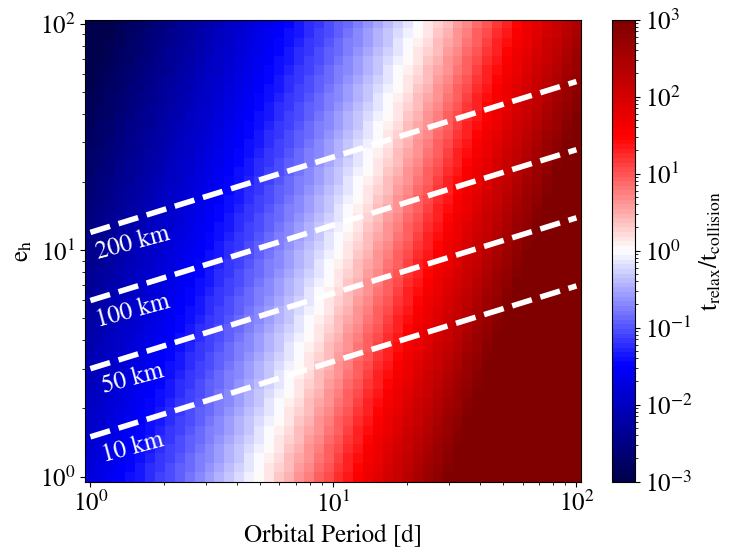
\includegraphics[width=0.5\textwidth]{figures/plStip/timescales.png}
    \caption{The ratio between the two-body relaxation and collision
      timescale for a population of equal-mass planetesimals with an
      internal density of 3 g cm$^{-3}$. The dashed curves show 
      the value of $e_{h}$ for which the random velocity dispersion is equal
      to the escape velocity of the planetesimals for a range of sizes. Only
      in regions where $t_{relax} \gg t_{coll}$ can the velocity distribution 
      respond to changes in the mass of the bodies such that oligarchic 
      growth can operate. This condition is no longer satisfied for a 
      dynamically hot disk at sufficiently short orbital periods.\label{fig:timescales}}
\end{center}
\end{figure}

\subsection{Planetesimal Size and Extent of Hill Sphere}\label{sec:sizeandhill}

In the formalism described above, the mass and velocity distribution
of the bodies are both a function of time. Due to the interdependence
of these quantities, it is not clear whether the ratio between the relaxation and collision timescales will remain constant as the
oligarchs develop. In the case of the solar system, $t_{relax} \ll t_{coll}$ likely continued to remain true, otherwise runaway 
growth would have consumed all of the small bodies and there would be nothing left to populate the asteroid or Kuiper belt. In 
the case where $t_{coll} \ll t_{relax}$, however, it is not clear how the system might evolve.

An insight into the expected behavior in this regime can be gained by
defining a dimensionless parameter, $\alpha$, which is the ratio
between the physical size of a body and its Hill radius, $r_{h}$
\begin{equation}\label{eq:alpha}
	\alpha = \frac{r_{pl}}{r_{h}} = \frac{1}{a} \left( \frac{9 M_{\star}}{4 \pi \rho_{pl}} \right)^{1/3},
\end{equation}
where $a$ is the semimajor axis of the body and $\rho_{pl}$ is its
bulk density. Assuming that the bulk density stays constant as bodies collide and
grow, and that no large-scale migration occurs, the scaling of both
$r_{pl}$ and $r_{h}$ as $m_{pl}^{1/3}$ means that $\alpha$ will be
constant with time. For a composition of ice and rock, $\alpha$ is
small for any presently populated region of the solar system ($\alpha \sim
10^{-2}$ near Earth and $\alpha \sim 10^{-4}$ in the Kuiper belt). As
one moves closer to the sun, $\alpha$ becomes larger than 1, which
implies that the Hill sphere of a body becomes smaller than its physical size.
As an additional note, the Roche limit of the central body and the distance at which $\alpha = 1$ are equivalent for a rigid spherical body. Applying a hydrostatic correction to the Roche limit, $a_{Roche} \simeq 0.6 a_{\alpha = 1}$. This accretion mode should therefore be relevant for ring systems, which is a topic that deserves further study using high resolution N-body techniques.

The magnitude of $\alpha$ controls the relative importance of gravitational scattering and collisions in driving the evolution of the planetesimal disk. When $\alpha$ is small, most close encounters will result in a gravitational interaction, moving the system toward a state of relaxation. If, however, the Hill sphere is largely filled by the body itself, these same encounters will instead drive evolution of the mass spectrum. Because $\alpha$ stays constant with mass, the boundary in the disk where collisions or gravitational encounters dominate, will stay static with time.

We also introduce a second dimensionless quantity, which relates the physical size of the bodies to the velocity state of the system
\begin{equation}\label{eq:beta}
	\beta = \frac{r_{pl}}{r_{g}}.
\end{equation}
where $r_{g} = G m_{pl} / v^{2}$ is the gravitational radius of a body (see eq 4.1 of \cite{ida90}). Encounters between bodies inside of a distance of $r_{g}$ result in significant deflections of their trajectories. It should be noted that the gravitational focusing enhancement factor $v^{2}/v_{esc}^{2}$ is equal to 1 for $\beta = 1$. In the case where $r_{g}$ is smaller than the size of a planetesimal, the gravitational focusing enhancement factor will be between 0 and 1 and the collision cross section is mostly set by the geometric value. For very large values of $r_{g}$ ($\beta \ll 1$), the effective collision cross section is almost entirely set by gravitational scattering.

These scaling considerations motivate the range of parameters we choose for the numerical experiments presented in the next section, where we aim to understand where and when runaway and oligarchic growth can operate. In figure \ref{fig:alpha_beta_diagram}, we show a schematic which relates $\alpha$ and $\beta$ to the geometry of a two-body encounter. For large values of $\alpha$, the Hill radius of a body (dashed circle) becomes comparable to its physical radius (solid circle). As $\beta$ increases, the trajectory of a body undergoing a flyby becomes more straight.

\begin{figure}
\begin{center}
    \includegraphics[width=0.5\textwidth]{figures/plStip/diagram.png}
    \caption{A diagram detailing how varying the values of $\alpha$ and $\beta$ affect the geometry of a two-body encounter. The solid circles represent the physical radius of a body and the dashed circles represent the Hill radius. As $\alpha$ is increased, the Hill radius and the physical radius become comparable in size. As $\beta$ is increased, the trajectory of a passing body for a fixed impact parameter is bent less and less.
      \label{fig:alpha_beta_diagram}}
\end{center}
\end{figure}

\begin{figure*}
\begin{center}
    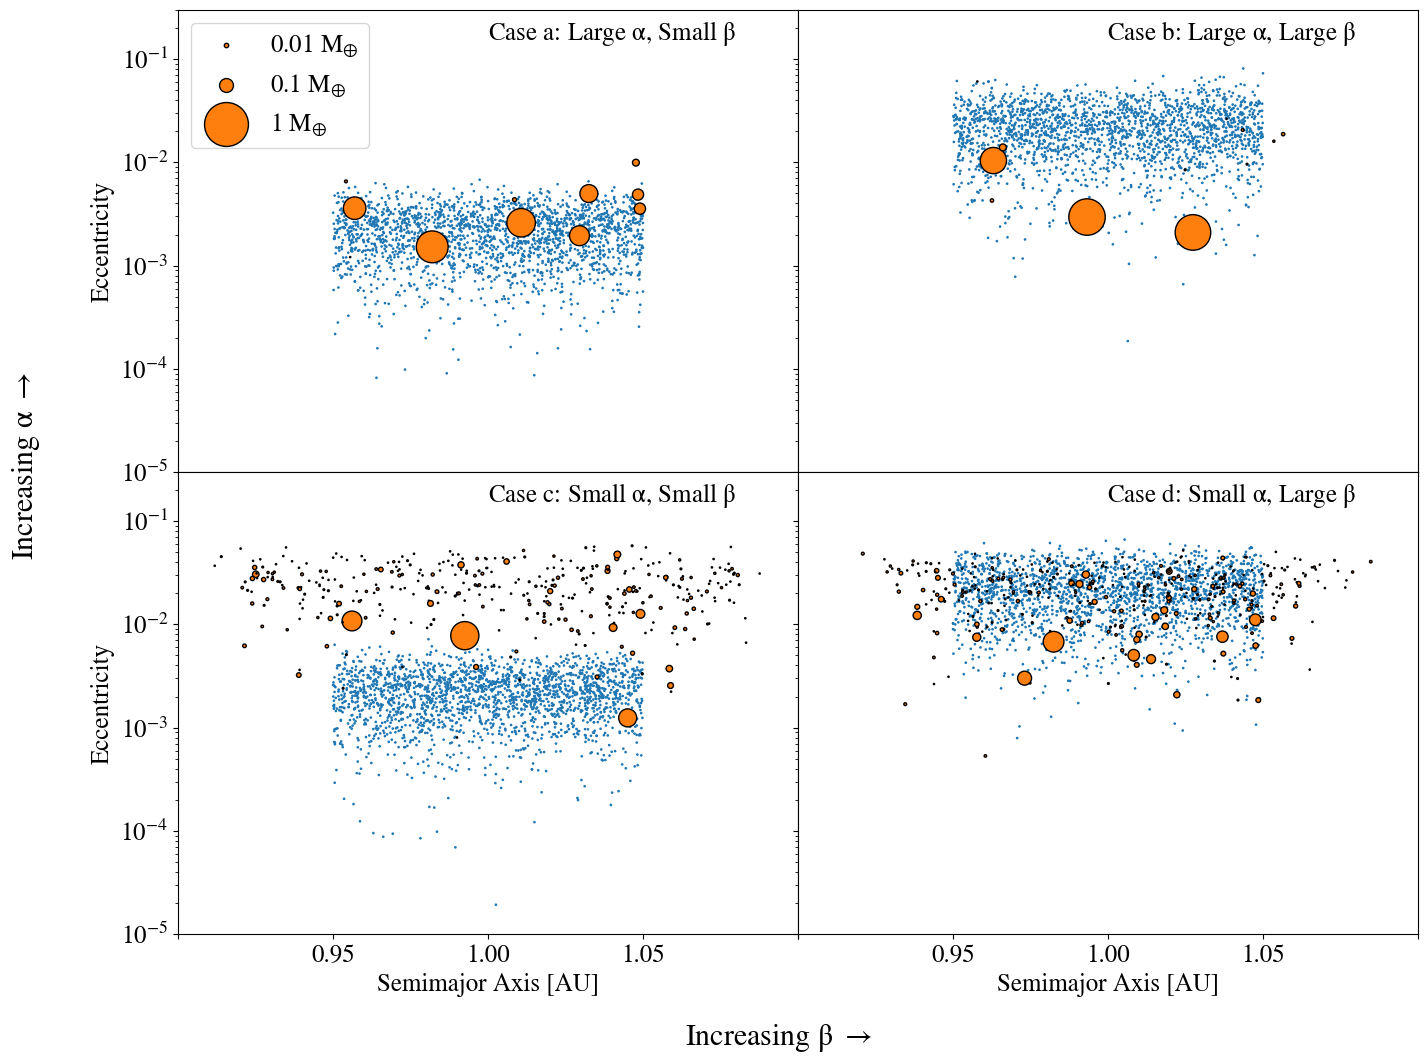
\includegraphics[width=\textwidth]{figures/plStip/alpha_beta.png}
    \caption{The initial (blue) and final (orange) states of the narrow annulus simulations described in section \ref{sec:narrow}. 
    Relative masses of the bodies are indicated by point size. In the case of large $\alpha$, almost no residual planetesimal 
    population remains. Regardless of the initial choice of $\beta$, the protoplanets that form attain similar eccentricities. 
    \label{fig:alpha_beta}}
\end{center}
\end{figure*}

\begin{figure}
\begin{center}
    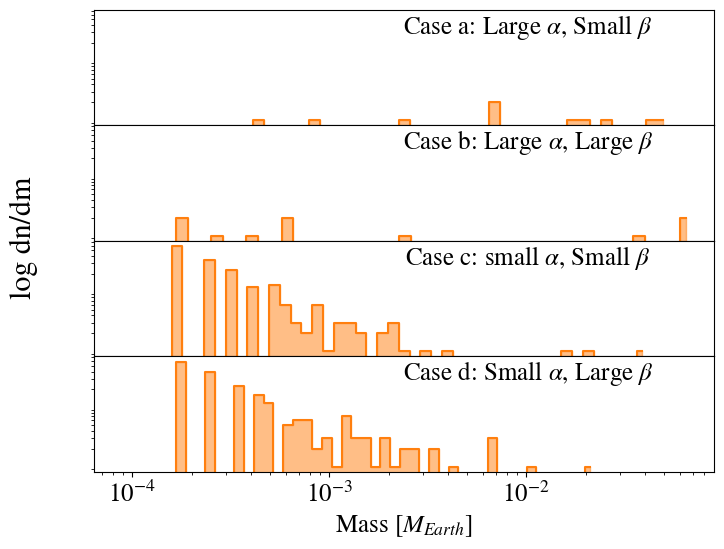
\includegraphics[width=0.5\textwidth]{figures/plStip/alpha_beta_mass.png}
    \caption{The final state of the mass distributions for the
      narrow annulus simulations described in section \ref{sec:narrow}. For small
      $\alpha$, a few embryos form alongside a power law tail of
      planetesimals. For larger values of $\alpha$, the mass distribution stops being bimodal. 
      As in the previous figure, the initial choice of $\beta$ does not appear to have any meaningful impact on the end result.
      \label{fig:alpha_beta_mass}}
\end{center}
\end{figure}

\begin{figure}
\begin{center}
    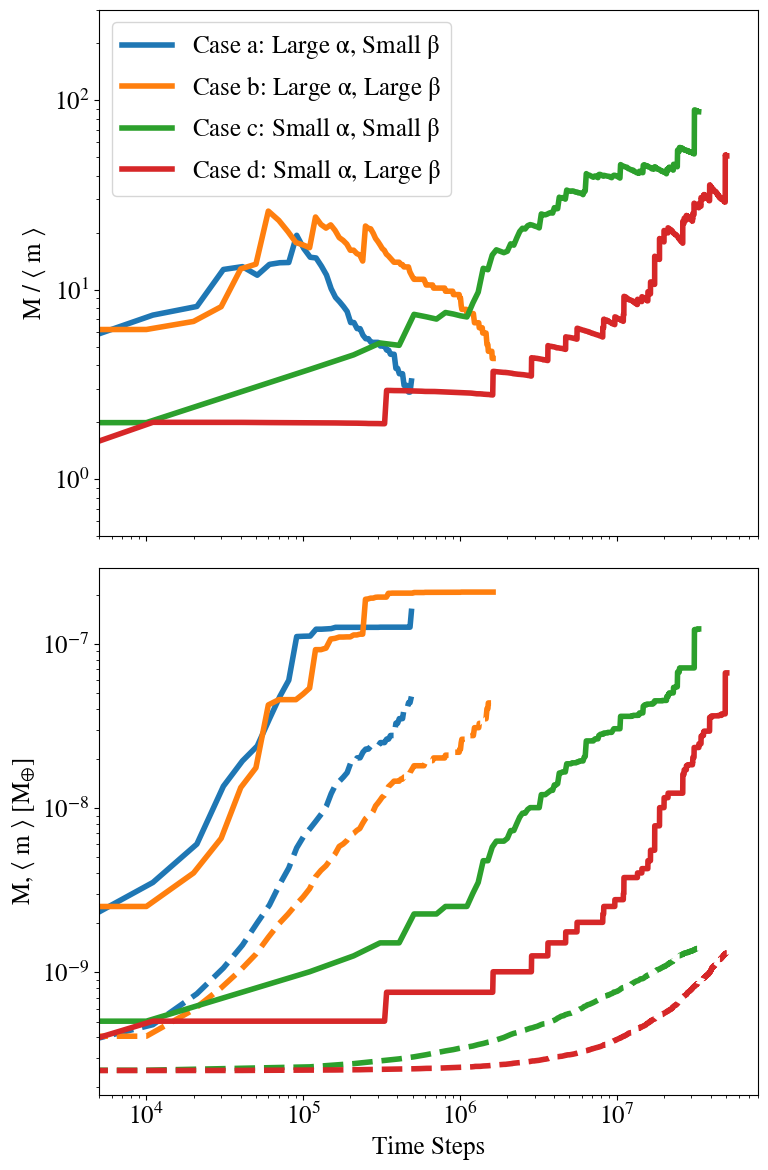
\includegraphics[width=0.5\textwidth]{figures/plStip/alpha_beta_evo.png}
    \caption{Top: The evolution of the ratio between the maximum and mean mass for the four simulations presented
    in section \ref{sec:narrow}. The runaway growth phase can be identified by a positive trend in this ratio. For all values of 
    $\alpha$, an increase in $\beta$ has the effect of delaying runaway growth. Bottom: The evolution of the maximum
    (solid lines) and mean (dashed lines) shown individually.\label{fig:alpha_beta_evo}}
\end{center}
\end{figure}

\section{Numerical Methods}\label{sec:methods}

We use the tree-based N-body code {\sc ChaNGa} to model the gravitational and collisional evolution of a swarm of planetesimals. A full description of the code, along with the details of the solid body collision module are provided in chapter \ref{ch:intro}. For all of the simulations presented below, we use a node opening criterion of $\Theta_{BH} = 0.7$. When modeling a wide planetesimal disk which spans two orders of magnitude in orbital period, we implemented a modified timestep criterion which is based on the perihelion distance of individual particles. The details of this implementation are described in section \ref{sec:timestep}.

\section{Narrow Annulus Simulations}\label{sec:narrow}

We begin by 
exploring the outcome of planetesimal accretion in different parts of the $\left( \alpha, \beta \right)$
parameter space. The choices of $\alpha$ and $\beta$ are motivated by two questions raised in section \ref{sec:theory}. 1) Does
runaway growth still operate when the condition that $v \ll v_{esc}$
is not satisfied? 2) How does planetesimal accretion proceed when the planetesimals themselves occupy a significant fraction of 
their Hill spheres?

To answer these questions, we run a series of simulations in which a
narrow annulus of planetesimals orbits a star. The values of $\alpha$
and $\beta$ are varied individually. 4000 planetesimals with
individual masses of $8.37 \times 10^{-5} M_{\earth}$ are placed with semimajor
axes drawn from a uniform distribution between 0.95 and 1.05 AU about a 1 $M_{\odot}$
star. In total, the disk contains $\sim$ 0.33 $M_{\earth}$ of material. The argument of perihelion, $\omega$, longitude of ascending node,
$\Omega$, and mean anomaly, M, for each body is drawn from a uniform
distribution $\in [0, 2 \pi)$. The inclinations and eccentricities are drawn
from a Rayleigh distribution with
$\left< i^{2} \right> = 1/2 \left< e^{2} \right>$ \cite{ida93a}.

In the ``fiducial'' case, we give the bodies a bulk density of 3 g
cm$^{-3}$ (for a radius of 341 km), and $\left< e^{2} \right>^{1/2} = 4 e_{h}$, which corresponds to $\alpha = 3.6 \times 10^{-2}$ and $\beta = 3.4 \times 10^{-3}$. These parameters are chosen to match the initial conditions of \cite{kokubo98}, which gave rise to oligarchic growth. 
To vary the value of $\alpha$, we alter the bulk density of the particles. In the high-$\alpha$ case, the bulk density is reduced by 
a factor of $\sim$ 7100, which produces $\alpha = 1$. This corresponds to a bulk density of $4.2 \times 10^{-4}$ g cm$^{-3}$ and a radius of 6,500 km. 
Although this is most certainly unphysical, the purpose of this modification is to have a planetesimal completely fills its Hill sphere so that no strong 
gravitational scattering should occur. To vary $\beta$, the eccentricity dispersion is increased. For the high-$
\beta$ case, $\left< e^{2} \right>^{1/2}$ is increased to $1500 e_{h}$, which corresponds to $\beta = 15,000$. This is the largest value of $\beta$ that permits a particle at 1 AU to still have an apocenter and pericenter distance that lies within the boundaries of the disk. This choice of $\beta$ places the system firmly in the $v > v_{esc}$ regime, while still allowing growth to occur in a reasonable number of timesteps.

In all cases, the simulations are evolved with a base timestep of 1.7
days, which corresponds to 3\% of an orbital dynamical time
$\sqrt{a^3/G M_{*}}$. Due to the vastly differing growth timescales in
each case, a simulation is stopped when the growth of the most massive
body flattens out. In figure \ref{fig:alpha_beta}, we show the a-e
distribution of bodies in the initial (blue) and final (orange)
snapshots from each of the 4 simulations. The size of the points
indicates the relative masses of the bodies. Only with small
$\alpha$ (case c, d) does a residual population of dynamically hot planetesimals
develop. The lack of high eccentricity planetesimals (relative to the protoplanets) in the large
$\alpha$ (case a, b) simulations suggests that most encounters result in accretion
rather than scattering. For large $\beta$ (case b, d), the growing protoplanets
end up in a dynamically cool state,
relative with the initial conditions. This is due to kinetic energy 
being lost as particles inelastically collide. One last point we note
is the difference between the eccentricities of protoplanets in the 
large $\alpha$, large $\beta$ (case b) and the small $\alpha$,
large $\beta$ (case d) simulation. The dynamically cooler result of the former case
is likely due to the dominant role that inelastic collisions play here.

In figure \ref{fig:alpha_beta_mass}, we show the mass distribution of bodies from the final snapshot in each of the four simulations. In addition to 
leaving fewer residual planetesimals, the large $\alpha$ (case a, b) simulations produce embryos that are a factor of a few larger. Despite the 
vastly different encounter velocities of each population of bodies, the initial size of $\beta$ (so long as bodies remain in the dispersion-dominated regime) 
appears to have no significant effect on the final distribution of masses. For reference, the boundary between shear and dispersion-dominated 
encounters ($e_{h}$ = 1) lies around e = $4 \times 10^{-4}$ for the planetesimal mass we have chosen. The eccentricity at which $\left< v^{2} \right>^{1/2} = 
v_{esc}$ for the planetesimals is around $10^{-2}$.

To investigate whether any of these planetesimal rings underwent
runaway growth, we examine the time evolution of the maximum and mean
masses in each simulation. The ratio $M/\left< m \right>$ is plotted
in the top panel of figure \ref{fig:alpha_beta_evo}. Here, a positive slope
indicates that the quantities are diverging (i.e.
the growth rate is accelerating with mass). This behavior is
evident in all four cases although the small $\alpha$ simulations eventually reach a stage where the curves
 turn over as the planetesimal supply depletes. Even with a large
$\beta$, where the effective collision cross section is
 nearly equal to the geometric value, runaway growth still appears to
operate. The ubiquity of the early positive trends in this figure suggests
that as bodies collide and grow, the
relative difference in gravitational focusing factors between bodies
is what drives the system towards runaway
growth, no matter how close the collision cross sections lie to the geometric value.
Although larger encounter velocities lengthen the growth
timescales, runaway growth appears to be inevitable, so long as
gravity is the dominant force in the system. For large $\alpha$
(case a, b), the curves in this figure eventually turn over and begin to decline.
In the bottom panel of figure \ref{fig:alpha_beta_evo}, we separately show the evolution of
the maximum (solid lines) and mean (dashed lines) mass for each case. Here, it is evident
that the turnover in $M/\left< m \right>$ is
driven by an increase in the average mass as the planetesimal population
becomes depleted. For small $\alpha$, one would expect that planetesimal accretion should also eventually come to a halt as
the growth timescale lengthens due to the planetesimal surface density decreasing and the residual bodies being scattered onto high
eccentricity orbits with negligible gravitational focusing factors. Many more timesteps, however, would be required to reach this point.

Additionally, these results suggest that the value of $\alpha$, which is a function of only the initial conditions, controls the qualitative outcome of accretion. 
Across most of a planet-forming disk, $\alpha$ is small, and frequent gravitational encounters between the growing bodies will 
facilitate oligarchic growth. In the dispersion-dominated regime, close encounters drive the stirring between planetesimals and 
embryos \cite{weidenschilling89, ida90}. When $\alpha \ll 1$, the Hill sphere of a body is mostly empty space and the majority of close encounters result in viscous stirring, rather than accretion. In the opposite regime, we 
observe that runaway growth still occurs, but nearly all of the planetesimals are consumed by the forming protoplanets, rather 
than being scattered onto higher eccentricity orbits, where they would otherwise remain as a remnant of the early stages of 
planet formation \cite{kokubo98, kokubo00}.

\section{Full Disk Simulation}\label{sec:fulldisk}

\subsection{Initial Conditions}

Motivated by the qualitative dependence of accretion on $\alpha$,
we next investigate whether this highly efficient, non-oligarchic
growth should be expected to operate near the innermost regions of a typical planet-forming
disk. Given that N-body simulations of short-period terrestrial planet formation 
typically begin with a chain of neatly-spaced, isolation mass 
(see \cite{kokubo00} eq. 20) protoplanets, it is pertinent to determine 
whether the high $\alpha$ growth mode we revealed
in the previous section invalidates this choice of initial conditions.

Given the dearth of short-period terrestrial planets observed around M stars (e.g. TRAPPIST-1 \cite{gillon16, gillon17, agol21}), we chose to model the evolution of a series of wide planetesimal disks, which span from 1 to 100 days in orbital period, orbiting a late-type M star of mass 0.08 $M_{\odot}$. For a population of planetesimals with a bulk density of 3 g cm$^{-3}$, this orbital period range corresponds to $\alpha \in (0.7, 0.05)$. By simultaneously modeling a broad range of orbital periods, we can determine the critical value of $\alpha$ that divides these two modes of accretion, and also explore how the oligarchic/non-oligarchic accretion boundary affects the resulting distribution of protoplanets.

Four wide-disk simulations are run in total (see table \ref{tab:sim_properties}). In each case, the solid surface density follows a power law profile
\begin{equation}
	\Sigma(r) = \textrm{10 g cm}^{-2} \times A \left( \frac{M_{*}}{M_{\odot}} \right) \left( \frac{r}{\textrm{1 AU}} \right)^{-\delta}
\end{equation}
where $M_{*}$ is the mass of the central star, 10 g
cm$^{-2}$ is the surface density of the minimum-mass solar nebula
\cite[MMSN]{hayashi81} at 1 AU, $A$ is an enhancement factor and $\delta$ is the power law index.
In the first case (fdHi), we model a disk that follows a MMSN power law slope ($\delta$ = 1.5), with the overall normalization enhanced by a factor of 100. This choice of normalization for the solid surface density profile appears necessary in order to reproduce many observed short period terrestrial worlds in-situ \cite{hansen12}. The most current planetesimal formation models all involve streaming instabilities triggered by solid material concentrating at preferential locations in the disk. This can occur via zonal flows \cite{johansen2009b, simon12}, vortices \cite{klahr03}, or through mechanisms that produce a pressure bump in the gas disk, such as an ionization \cite{lyra08} or condensation front \cite{brauer08b, drkazowska13}, or even the perturbations from an existing planet \cite{shibaike20}. \cite{drkazowska18} showed that evolution of the snow line boundary can cause planetesimal formation over a significant area of the disk, producing mass concentrations at least as large as the ones we use here. We argue that this is a particularly attractive mechanism for widespread planetesimal formation around low-mass stars, as their extreme pre-main sequence evolution is particularly conducive to significant movement of the condensation fronts \cite{baraffe15}.

Additionally, we vary the power law index (fdHiShallow, fdHiSteep) and overall normalization (fdLo) of $\Sigma(r)$. Although there is no way to reliably measure the uncertainty on the MMSN power law slope, \cite{chiang13} applied a similar analysis to a sample of Kepler multiplanet systems and found a variation of $\sim 0.2$. Sub-millimeter observations of the outer regions of cold protoplanetary disks find that $\delta$ can be as low as 0.5 \cite{mundy00, andrews09, andrews10}. Therefore, we vary $\delta$ by a value of $1.0$ relative to the MMSN value for the fdHiShallow and fdHiSteep simulations.

In all cases, the eccentricities and inclinations of the bodies are randomly drawn from a Rayleigh distribution, with $\left< e^{2} \right>^{1/2} = 2\left<i^{2} \right>^{1/2} = e_{eq}$ \cite{ida93}. Following \cite{kokubo98}, the value of $e_{eq}$ is chosen such that the timescales for viscous stirring and aerodynamic gas drag on the planetesimals are in equilibrium. Although this approach assumes that these two mechanisms are in balance, there is nothing preventing planetesimal accretion from getting underway before the disk is sufficiently hot to be limited by gas drag. However, as we showed in the previous section, the initial dynamical state of the planetesimals does not seem to affect the outcome of accretion, so it is safe to assume that the resulting distribution of protoplanets would remain unchanged had we started with a colder disk. The viscous stirring timescale is given by \cite{ida93} as

\begin{equation}\label{eq:vs_timescale}
    t_{vs}  = \frac{\left< e^2 \right>}{d \left< e^2 \right> / dt} \approx \frac{1}{40}\left(\frac{\Omega^{2} a^{3}}{2 G m_{pl}}\right)^{2} \frac{4 m_{pl} \langle e^{2} \rangle^{2}}{\Sigma a^{2} \Omega},
\end{equation}
where $\Omega$, $a$ and $e$ are the orbital frequencies, semi-major axes and eccentricities of the individual planetesimals, respectively. In the Stokes regime, where the mean-free path of the gas is much smaller than the solid particles, the gas can be treated as a fluid and the drag timescale is given by \cite{adachi76} as

\begin{equation}\label{eq:ts_stokes}
    t_{s} = \frac{2 m_{pl}}{C_{D} \pi r_{pl}^{2} \rho_{g} v_{g}},
\end{equation}

where $C_{D}$ is a drag coefficient of order unity, $\rho_{g}$ is the local gas volume density and $v_{g}$ is the headwind velocity of the gas experienced by the planetesimal. The local gas volume density is given by
\begin{equation}\label{eq:rho_gas}
	\rho_{g} = \frac{\Sigma_{g}}{\sqrt{2 \pi} h_{g}} \exp\left[ -z^{2} / \left( 2 h_{g}^{2} \right) \right],
\end{equation}
where $\Sigma_{g}$ is the gas surface density (taken to be
240 times the solid surface density \cite{hayashi81}, $h_{g} = c_{s} / \Omega$ is the local gas scale height and $z$ is the height above the disk midplane. The sound speed profile is given by $c_{s} = \sqrt{k_{B} T(r) / \left( \mu m_{H} \right)}$, where $k_{B}$ is Boltzmann's constant, $T(r) = T_{0} \left( r / 1 \textrm{AU} \right)^{-q}$, $\mu = 2.34$ and $m_{h}$ is the mass of a hydrogen atom. For a protoplanetary disk around a typical M star, $T_{0} = 148$ K and $q$ = 0.58 \cite{andrews05}.

Finally, the headwind velocity of the gas, due to the fact that the gas disk is pressure supported, is given by

\begin{equation}\label{eq:v_gas}
	v_{g} = v_{k} \left[ 1 - \sqrt{ q c_{s}^2 / v_{k}^2} \right],
\end{equation}

\noindent where $v_{k}$ is the local Keplerian velocity (see eq. 4.30 of \cite{armitage20}). As in section
\ref{sec:narrow}, the argument of perihelion $\omega$, longitude of
ascending node $\Omega$, and mean anomaly M for the planetesimals are drawn from a uniform distribution $\in [0, 2 \pi)$.

One should note that this choice for the gas disk profile almost certainly does not capture the wide range of possibilities in real planet-forming disks. 
On one hand, a larger initial gas surface density could act to completely remove solids via radial drift, rendering in-situ accretion of solids impossible. On the 
other hand, a more tenuous gas disk might render aerodynamic drag forces completely unimportant. In this case, the random velocity of the initial 
planetesimals should be close to their mutual escape velocity. As we showed in section \ref{sec:narrow}, the initial dynamical state of the solids seems to 
have a very minimal effect on the final outcome of planetesimal accretion. In a similar vein to \cite{hansen12}, we choose to use a MMSN-like profile for the 
gas disk and instead vary the solid surface density profile to capture the range of mechanisms that might have acted to facilitate planetesimal formation in the 
first place.

\subsection{Gas Drag Force}

In addition to the mutual gravitational forces, a Stokes drag force
due to the the gas disk is applied to each particle, following the
prescription described in section 2.2.1 of \cite{morishima10}. For
the initial mass planetesimals, the Stokes number
  ($\textrm{St} = t_{s} \Omega$) at the inner and outer disk edge is
  roughly $2 \times 10^{5}$ and $10^{7}$, respectively. For $t_{s} \gg
  1$, bodies are decoupled from the gas and are only weakly affected
  by it. Because $t_{s} \sim m^{1/3}$, the Stokes number grows as planetesimal accretion proceeds, and the drag force plays an increasingly minor role. Although the aerodynamic gas drag is not expected to significantly alter the final protoplanet distribution, we include its effects here to be self-consistent with the initial conditions, which were constructed by balancing the effects of viscous stirring with gas drag.

\subsection{Timestepping Criterion}\label{sec:timestep}

In the case of the fdHi simulation, there are nearly 1 million
particles, whose orbital periods vary by two orders of magnitude. Because the
interaction timescales near the inner edge of the
disk are exceedingly short, a fixed timestep size would required a prohibitively large
number of steps to follow planetesimal growth throughout the entire
disk. For this reason, we use a multi-tiered timestepping scheme, in
which particles are placed onto the nearest power of two timestep
based on their most recently calculated gravitational
acceleration. This scheme is used on almost all works using ChaNGa,
and is common among large-scale simulation codes.

This more efficient scheme introduces two issues, however. Firstly,
momentum is not completely conserved when bodies switch timestep tiers. The
error introduced becomes particularly severe for a particle on an
eccentric orbit, whose perihelion and aphelion distances
straddle a timestep boundary. For a large collection of particles,
this problem manifests itself as the development of a V-shaped gap in the a-e plane, centered on the boundary itself. To correct this problem, we introduce a slightly modified timestepping criterion, which is based on the expected gravitational acceleration of the particle at pericenter. Only in the case of a close encounter with another planetesimal (in which the acceleration is no longer dominated by the star) is the timestep allowed to reduce based on the original instantaneous criterion.

A second issue is introduced when two particles on different timesteps
undergo a collision. As in the previous case, momentum is not
completely conserved because the most recent `kick' steps did not
happen simultaneously for these bodies. Early in the simulation, we
find that this problem tends to trigger runaway growth at the timestep
boundaries first. This issue carries itself forward through the embryo
formation phase, and protoplanets tend to form at the boundaries. To
correct this issue, we ignore collisions between bodies on different
timesteps early in the simulation. We find that preventing
multi-timestep collisions until after the maximum mass grows by a
factor of 10 prevents any artifacts from developing at the timestep
boundaries, while also minimizing the number of `skipped' collisions. In the case of the fdHi simulation, only about 20 collisions out of an eventual 900,000 are ignored. To verify that this timestepping scheme does not affect protoplanet growth, we tested an annulus of growing planetesimals with both fixed steps and our two-phase variable timestepping scheme. The results of these tests are shown in section \ref{sec:rung_ecc}.

\begin{figure}
\begin{center}
    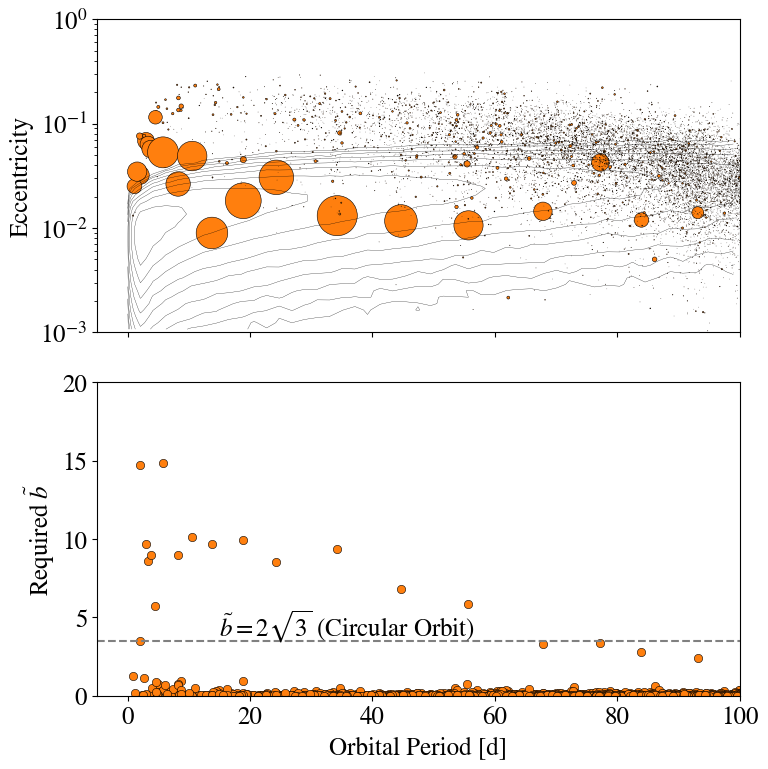
\includegraphics[width=0.5\textwidth]{figures/plStip/fulldisk_e_m_b.png}
    \caption{The final state of the fdHi simulation. In the top panel,
      the contours denote the initial period-eccentricity distribution
      of the planetesimals. Point sizes indicate the relative masses
      of bodies at the end of the simulation. In the bottom panel, we show the
      feeding zone width (see equation \ref{eq:iso}) required to produce
      the final masses of the bodies. The dashed line indicates the feeding
      zone size expected for bodies on circular orbits. For the shorter period bodies,
      the feeding zone size exceeds this expected value, which indicates that oligarchic growth is
      not operating here. This boundary occurs near roughly 60 d in orbital period.\label{fig:fulldisk_e_m}}
\end{center}
\end{figure}

\begin{figure}
\begin{center}
    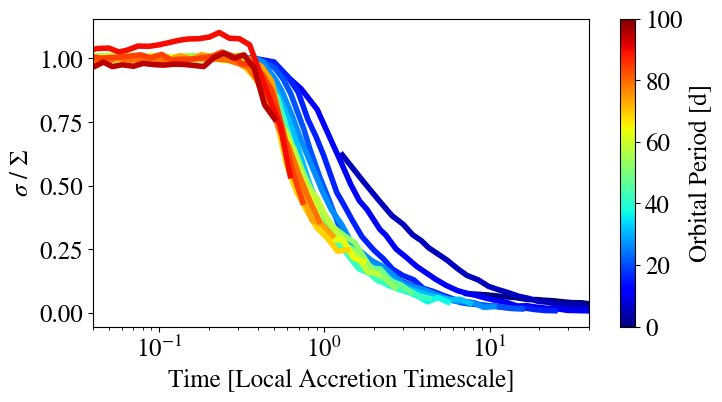
\includegraphics[width=0.5\textwidth]{figures/plStip/pl_frac_time.png}
    \caption{The time evolution of the planetesimal surface density (in units of the total solid surface density) in the fdHi 
    simulation. Each curve represents a radial slice of the disk. The time is measured in units of the local accretion 
    timescale at the center of each radial zone. The colors represent the orbital period at the center of each zone.\label{fig:pl_frac_time}}
\end{center}
\end{figure}

\begin{figure}
\begin{center}
    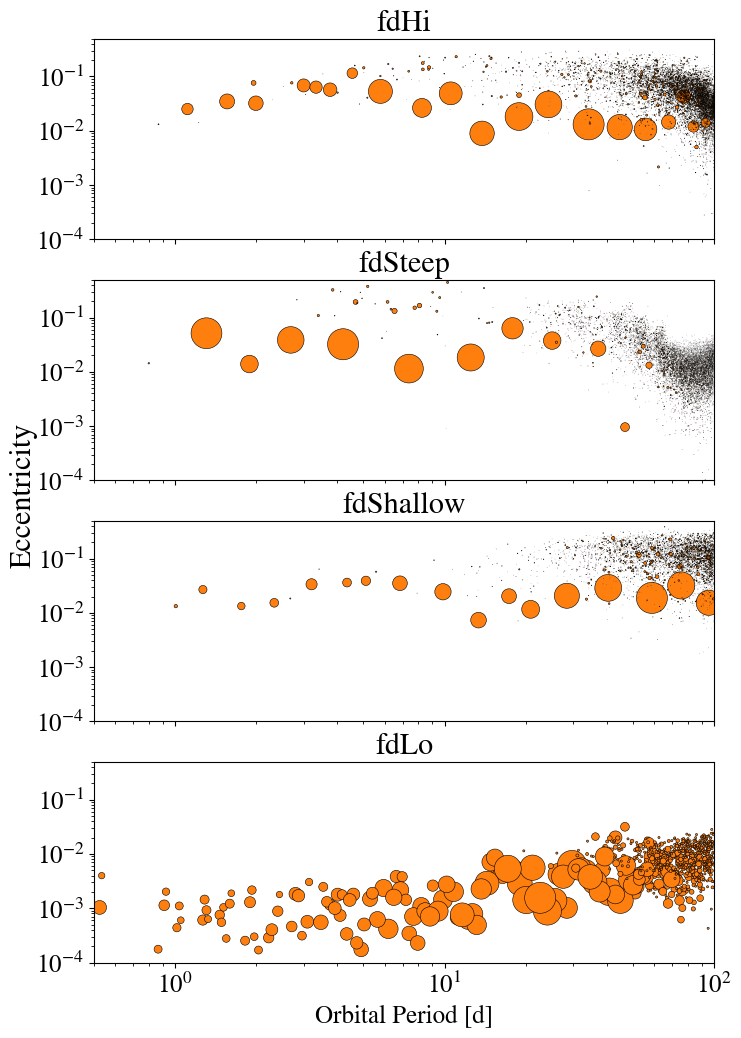
\includegraphics[width=0.5\textwidth]{figures/plStip/surfden_profiles.png}
    \caption{The final state of the full disk simulations listed in table \ref{tab:sim_properties}. 
    Point sizes indicate mass relative to the largest body in each simulation.\label{fig:surfden_profiles}}
\end{center}
\end{figure}

\begin{figure}
\begin{center}
    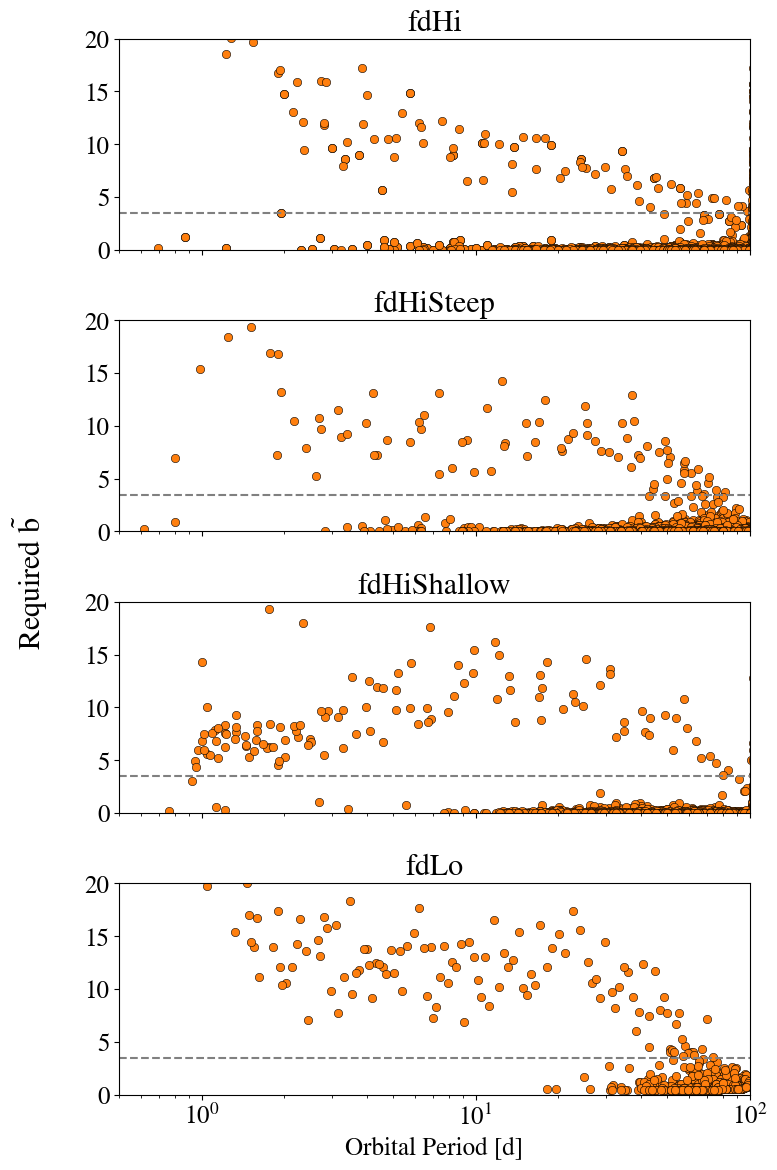
\includegraphics[width=0.5\textwidth]{figures/plStip/surfden_b.png}
    \caption{Feeding zone width (see equation \ref{eq:iso}) required to produce the final masses for the protoplanets from the 
    simulations listed in table \ref{tab:sim_properties}. For the fdHi, fdHiSteep and fdHiShallow simulations, we have included the results from five separate iterations of the simulations, each using a different random number seed. The horizontal dashed line indicates $\tilde{b} = 2 \sqrt{3}$. Despite the 
    vastly different initial solid surface density profiles, the feeding zone width reaches the circular orbit value around $\sim$ 60 
    days in all cases. \label{fig:surfden_b}}
\end{center}
\end{figure}

\subsection{Results}

\begin{table*}
\begin{center}
\caption{Summary of Full Disk Simulations}
\begin{tabularx}{1.0\textwidth}{l@{\extracolsep{\fill}}ccccccc} \hline \hline
Simulation Name & $m_{pl} [M_{\earth}]$ &$N_{pl}$ & A & $\delta$ & $M_{PP}  [M_{\earth}]$ & $T_{int} [yr]$ & $T_{int, 1} [yr]$ \\ \hline
fdHi              & $8.37 \times 10^{-6}$ & 903,687 & 100 & 1.5 & 1.00 & 456 & 16,377  \\
fdHiSteep    & $8.37 \times 10^{-6}$ & 903,687 & 100 & 2.5 & 1.19 & 456 & 16,377  \\
fdHiShallow & $8.37 \times 10^{-6}$ & 903,687 & 100 & 0.5 & 1.08 & 456 & 16,377 \\
fdLo             & $8.37 \times 10^{-6}$ & 45,185  & 1      & 1.5 & $1.77 \times 10^{-3}$ & 3,713 & 133,651 \\ \hline
\end{tabularx}\\
\begin{flushleft}
\textit{Note:} A summary of the four `full disk' simulations presented in section \ref{sec:fulldisk}. $m_{pl}$ and $N_{pl}$ are the initial masses and number of planetesimals. $A$ and $d$ is the initial power law normalization and slope of the solids in the disk. $M_{PP}$ is the maximum protoplanet mass at the end of the simulation and $T_{int}$ is the amount of time each simulation was integrated. $T_{int, 1}$ is the integration time scaled by a factor of $f^{2}$, which accounts for the fact that the accretion timescale has been shortened by the inflated collision cross sections.
\end{flushleft}
\label{tab:sim_properties}
\end{center}
\end{table*}

The timescales for embryo formation depend on
the chosen surface density profile, along with the local orbital
timescale. Protoplanets form first at the inner edge of the disk,
where the dynamical timescales are short. Growth proceeds in an
inside-out fashion, with the outermost regions of the disk completing
the protoplanet assembly phase last (as an example, see figure 1 of \cite{kokubo02}). This radial timescale dependence is not typically
accounted for in planet formation simulations a notable exception being \cite{emsenhuber21a, emsenhuber21b}, and appears to be an
important component to forming realistic solar system analogs
\cite{clement20}. As with the narrow annulus simulations, we stop the
integration once the masses of protoplanets in the outermost region of
the disk reach a steady value. In table \ref{tab:sim_properties}, we
summarize the outcomes of the four ``full disk'' cases.

We show the final state of the ``fdHi'' simulation in figure \ref{fig:fulldisk_e_m}. In the top panel,
the initial (contours) and final (points) state of the simulation is
shown in the orbital period-eccentricity plane. The size of the points
indicates the relative mass of the bodies. In the bottom panel, the
final masses of the bodies (in units of feeding zone size $\tilde{b}$) are shown
as a function of orbital period. The y-values in the bottom panel of figure \ref{fig:fulldisk_e_m} are calculated by solving equation \ref{eq:iso} for $\tilde{b}$, and inputting the initial surface density and final particle mass into the expression. In other words, $\tilde{b}$ is describing the size of the annulus that must be cut out of the planetesimal disk in order to produce a protoplanet of the current mass. By plotting the derived value of $
\tilde{b}$ as a function of orbital period, differences in the dynamical interactions at different locations of the disk are made more 
clearly visible. The feeding zone size $\tilde{b} = 2 \sqrt{3}$ permitted by bodies on circular, non-inclined orbits \cite{naka88} is shown by the
horizontal dashed line. In typical oligarchic growth simulations \cite{kokubo98}, protoplanets tend 
to space themselves apart by $\tilde{b} = 10$, although it should be noted that they do not consume all of the planetesimals 
within this distance.

A qualitative shift in the protoplanet and planetesimal distribution is visible inside of $\sim$ 60 days. Interior to this location, there are 
very few remaining planetesimals and the embryos formed have larger feeding zones. Exterior to the boundary, the residual 
planetesimal population is much more visible, and protoplanets more closely follow the $\tilde{b} = 2 \sqrt{3}$ line. This 
suggests that the transition between the low $\alpha$ and high $\alpha$ accretion modes seen in section \ref{sec:narrow} 
is happening near this location.

In section \ref{sec:narrow}, we postulated that the increased importance of inelastic damping in the inner, non-oligarchic growth 
region of the disk should lower the overall eccentricity of the protoplanets there. This behavior is not immediately apparent in the 
top panel of figure \ref{fig:fulldisk_e_m}. In fact, the opposite appears to be true. There are, however, a couple of factors in the wide disk simulations that could make this 
extra dynamical cooling mechanism difficult to see. Firstly, the initial eccentricity distributions of the inner and outer disk are 
different because of the dependence of the viscous stirring and gas drag timescales on orbital period. The mean eccentricity at the outer disk edge is 4x larger than at the inner disk edge. Additionally, the 
protoplanet formation timescales for the inner and outer disk are vastly different, making a comparison between these regions at 
the same moment in time somewhat inappropriate. A quick back of the envelope calculation yields $\left< e^2 \right>^{1/2} = 0.05$ for a population of $\sim 1 M_{\earth}$ bodies with a random velocity dispersion equal to their mutual escape velocity. It is therefore likely the case that the innermost protoplanets have had ample time to self-stir.

To ensure that the boundary seen around 60 days in orbital period is not
simply a transient product of the inside-out growth throughout the
disk, we examine the time evolution of $\sigma/\Sigma$, which compares the planetesimal and total solid surface density at 
multiple orbital periods. In figure \ref{fig:pl_frac_time}, the value of
$\sigma/\Sigma$ is plotted as a function of time in 10 orbital period
bins, each with a width of 10 days. To determine whether the evolution of the planetesimal surface density behaves self-similarly across the disk,
we normalize the time values in each bin by the local accretion timescale at the beginning of the simulation, which is given by

\begin{equation}\label{eq:acctime}
	t_{acc} = \left( n \Gamma v \right)^{-1} = \left( \frac{\Sigma_{0} \Omega}{2 m_{pl}} \Gamma \right)^{-1},
\end{equation}

\noindent where we have assumed the local number density of particles n is set by the surface density and the local scale height of the disk (see section \ref{sec:theory}). The effective collision cross section is set by gravitational focusing and is given by equation \ref{eq:gravfocus}.

The color of the curves indicate the orbital period bin which is being measured. From about 40 to 100 days in orbital period, the planetesimal surface 
density follows a similar trajectory as accretion proceeds. Interior to about 40 days, $\sigma$ actually decays more slowly. In other words, growth is actually 
fueled less vigorously by planetesimals in this region. This highlights the fact that accretion proceeds in a qualitatively different way in the inner disk. For the 
outer disk, gravitational focusing tends to facilitate collisions between protoplanets and preferentially smaller bodies. At short period, however, all close 
encounters result in a collision, regardless of mass. In a rather counterintuitive fashion, planetesimals in the inner disk actually persist for longer. In section 
\ref{sec:assembly}, we examine the assembly history of the embryos and show that there is much less of a preference for planetesimal-embryo collisions at 
short period as well.

In the inner disk, this value asymptotes to zero as the 
planetesimal population entirely depletes. In the outer disk, dynamical friction between the embryos and planetesimals 
eventually throttles subsequent accretion and leaves $\sim$ 10 percent or more of the mass surface density as planetesimals. It 
should be noted that in a typical oligarchic growth scenario, where protoplanets space themselves apart by 10 $r_{h}$ and settle 
onto circular orbits (giving $\tilde{b} = 2 \sqrt{3}$), roughly 30 percent ($2\sqrt{3}/10 \simeq 0.3$) of the planetesimals
should remain out of reach of the protoplanets.

Next, we investigate how the resulting planetesimal and protoplanet distribution
changes as we vary the initial solid surface density profile.
The final orbital period-eccentricity state of the
particles in the fdHi, fdHiSteep, fdHiShallow and fdLo simulations are shown in figure \ref{fig:surfden_profiles}, with point sizes 
indicating the relative masses of the bodies. In all cases, the inner disk is largely depleted of planetesimals, while the outer disk 
contains a bimodal population of planetesimals and embryos, with a clear separation in eccentricity between the two. Despite 
having significantly different masses, the semimajor axis-eccentricity distributions of the planetary embryos formed in all simulations are remarkably similar. This 
is likely due to the fact that inelastic collisions play a more significant role where the solid surface density is highest, which 
offsets the fact that the initial bodies started off in a dynamically hotter state (due to the increased effectiveness of viscous stirring). The only exception to this is the fdLo simulation, 
where the resulting eccentricities are a couple orders of magnitude smaller. Inelastic damping likely plays an even more 
significant role here, due to the much larger masses of the initial planetesimals.

In figure \ref{fig:surfden_b}, we plot the masses of the resulting protoplanets and planetesimals in all four simulations in units of $
\tilde{b}$ (see equation \ref{eq:iso}). To make the trend between $\tilde{b}$ and orbital period more clear, we ran four more versions of the fdHi, fdHiSteep and fdHiShallow simulations using different random number seeds and included these in the figure as well.
As mentioned previously, $\tilde{b} = 2 \sqrt{3}$ (indicated by the horizontal dashed line) is the  
feeding zone width that a body on a circular orbit will have. In all four simulations, the feeding zone width exceeds the 
minimum value in the inner disk and approaches $2 \sqrt{3}$ around $\sim$ 40 to 60 days. The orbital periods at which this transition 
occurs are quite similar between simulations, despite the vastly different solid surface density profiles used. This indicates that 
the boundary between accretion modes is driven entirely by the local value of $\alpha$, and also supports our 
conclusion that planetesimal accretion is largely complete everywhere in the disk.

\subsection{Assembly History of Embryos}\label{sec:assembly}

Further insight regarding the difference between the short vs long period accretion modes can be gained by looking at the 
growth history of the planetary embryos. Because all collisions are directly resolved by the N-body code, a lineage can be 
traced between each planetary embryo and the initial
planetesimals. For the fdHi, fdHiSteep and fdHiShallow
  simulations, protoplanets gain a factor of $\sim 10^6$ in mass
  relative to the initial planetesimals. For the fdLo simulation, this growth factor is nearly a thousand times smaller, which produces rather shallow and noisy collision histories. For this reason, we choose to exclude the fdLo simulation from our analysis in this section.

We begin by investigating the ``smoothness'' of the accretion events
that give rise to each embryo. Drawing from a common technique used
for cosmological simulations of galaxy formation, we divide growth events for
a given body into ``major'' and ``minor'' mergers \cite{kauffmann93, murali02, lhullier12}. 
Here, we define minor events as any collision involving an initial mass 
planetesimal, while major events consist of a merger between any two larger bodies.
In figure \ref{fig:minor_frac}, we retrieve the collision events for all bodies in all five iterations of the fdHi, fdHiSteep and fdHiShallow
simulations and plot the total mass fraction attained through minor merger (smooth accretion) events as a function of the final mass of the body. Here, we define a minor merger
to be any collision involving a planetesimal with $m < 100 m_{0}$. The color of the
points indicates the final orbital period of the body. Beyond $\sim$ 20 to 30 days in orbital period, minor mergers make up a significant fraction of the final mass of a body. Interior to this, the smooth accretion fraction drops significantly and the mass contribution to minor mergers can vary by over an order of magnitude.

\begin{figure}
\begin{center}
    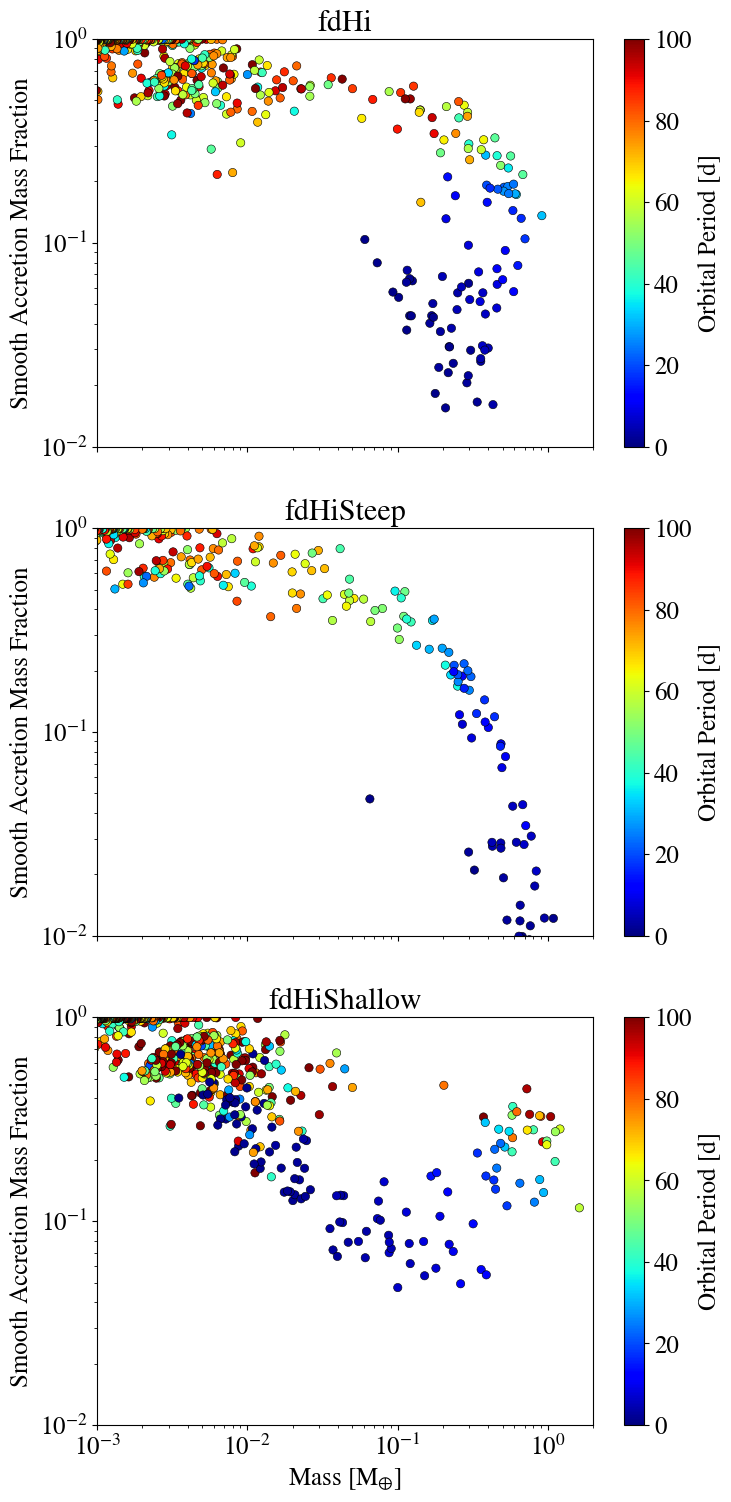
\includegraphics[width=0.5\textwidth]{figures/plStip/minor_frac.png}
    \caption{For all bodies with $m > 100 m_{0}$ at the end of the high surface density simulations, the fraction of their total mass attained through mergers with initial mass planetesimals (smooth accretion) as a function of total mass. Colors indicate the orbital periods of the bodies in the final simulation snapshot. Bodies interior to $\sim$ 20 to 30 days attain up to an order of magnitude less of their mass through minor merger events, while accretion of planetesimals plays a much more significant role at longer orbital periods.\label{fig:minor_frac}}
\end{center}
\end{figure}

\begin{figure}
\begin{center}
    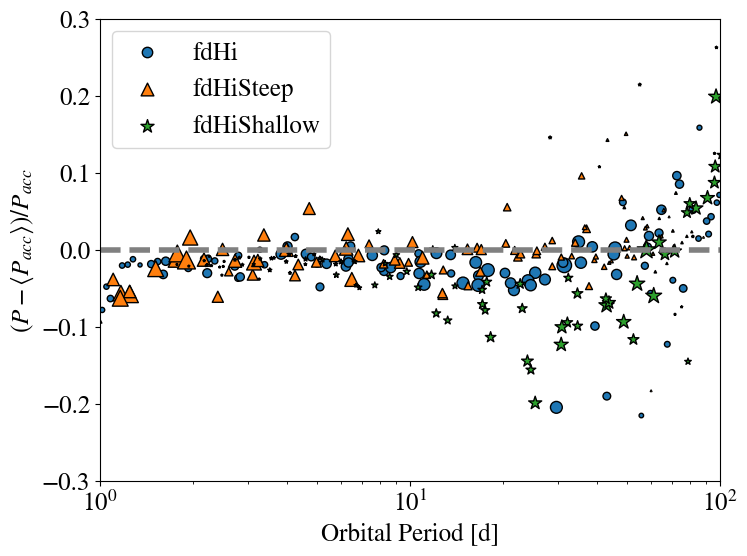
\includegraphics[width=0.5\textwidth]{figures/plStip/acc_zones.png}
    \caption{The relative separation between the final period
        of a body and the mean orbital periods of its accretion zone at the end of the fdHi, fdHiSteep and fdHiShallow simulations. The marker type and color denotes the simulation used, while the marker sizes indicate the relative masses of bodies. In each case, all five iterations of the simulations are plotted simultaneously.\label{fig:acc_zones}}
\end{center}
\end{figure}

The variation in smooth accretion fraction with mass for the short period bodies suggests that the planetesimal and embryo populations interact differently than those in the outer disk. Exterior to the accretion mode boundary, the growing embryos continue to accrete planetesimals while avoiding each other as they near their final mass. Inside the boundary, however, any and all bodies collide with each other, and the occasional embryo-embryo collision tends to dominate growth and drive down the smooth accretion fraction. Gravitational scattering between embryos and planetesimals is a key ingredient for orbital repulsion \cite{kokubo98}, and so a lack of gravitational scattering in the inner disk should prevent the embryos from settling onto neatly-spaced, isolated orbits. As we showed in figure \ref{fig:surfden_b}, the embryos in the inner disk appear to reach well beyond the typical feeding zone size predicted by an oligarchic growth model. Figure \ref{fig:minor_frac} suggests that the extra mass here obtain comes from mergers with the other nearby embryos.

Another line of evidence pointing to a lack of gravitational
scattering and orbital repulsion in the inner disk can be seen in
figure \ref{fig:acc_zones}. Here, we measure the initial orbital period distribution of bodies used to construct each embryo and calculate its mean $\left<  P_{acc} \right>$. Point sizes indicate the relative final masses of bodies. As in the previous figure, we have included data from all five versions of the fdHi, fdHiSteep and fdHiShallow simulations. For each body, this quantity is then compared with its final orbital period. In this figure, bodies that closely follow the gray dashed line still reside close to their initial feeding zones. On the other hand, bodies further from the dashed line must have experienced a strong gravitational scattering event during or after their accretion has completed. For all of the high surface density simulations, the accretion zones and present positions of the embryos appear to diverge beyond $\sim$ 20 days in orbital period.

Coupled with the strong decrease in smooth accretion fraction for bodies in this region (seen in figure \ref{fig:minor_frac}), it appears as if the relative importance of collisions and gravitational scattering seems to shift around $\sim$ 20 days. For the shortest period bodies, growth events are sudden and stochastic, often involving collisions between bodies of comparable mass. For longer period bodies, a significant amount of growth is driven by accretion of smaller planetesimals. We postulate that this qualitative difference is driven by the role that embryo-embryo close encounters play in the inner and outer disk. In the inner disk, these encounters tend to result in a merger, which drives down the smooth accretion fraction. In the outer disk, these encounters tend to result in a scattering event which moves bodies away from their initial feeding zones. We find that the accretion zone shapes for the longer period bodies are also much more smooth and unimodal, which suggests that scattering tends to occur after accretion has largely completed.

\section{Simplifying Assumptions}\label{sec:assump}

\subsection{Collision Cross Section}

In all cases shown so far, the boundary between the
oligarchic growth and the highly-efficient short period accretion
region lies between 40 and 70 days in orbital period. As discussed in section \ref{sec:sizeandhill}, the mode of accretion is
set entirely by the local value of $\alpha$, which scales with both
distance from the star and the bulk density of the planetesimals (see
equation \ref{eq:alpha}). Because we chose to artificially inflate the
collision cross section of the particles in our simulations by a factor of $f$, the bulk densities
of the particles are reduced, and the accretion boundary is shifted outward.
However, the scaling relation between $\alpha$ and $\rho$ ($\alpha \sim \rho_{pl}^{-1/3}$) can be used
to predict where this accretion boundary should lie in a disk with realistic-sized planetesimals. The simulations
presented in this chapter use a collision cross section enhancement factor of 6, which moves the boundary outward in orbital
period by a factor of approximately 15 (For a fixed value of $\alpha$, equation \ref{eq:alpha} gives $a \sim r_{pl} \sim f$ and therefore $P_{orbit} \sim f^{-3/2}$). One would therefore expect the accretion boundary to lie between 3 and 5 days in orbital period
for 3 g $cm^{-3}$ bodies.

Although a simulation with $f=1$ is not computationally tractable, we
can test whether the accretion boundary moves in the way we expect by
modestly changing the value of $f$. In figure \ref{fig:f6f4_b}, we
compare the fdHi simulation to a nearly identical run using $f=4$. In
the top panel, we show the feeding zone width required for each particle to
attain its present mass. As in figure \ref{fig:surfden_b}, we indicate the feeding
zone size expected for oligarchic growth with a horizontal dashed line. In the bottom panel, the value
of $\alpha$ as a function of orbital period is shown for 3 g $cm^{-3}$
bodies with an artificial radius enhancement of $f=1$, 4 and 6. The
horizontal dashed line indicates the empirical value of alpha below which the
accretion mode switches to oligarchic. Comparing the top and
bottom panels, the intersection of the feeding zone width seen in our simulations and the
feeding zone width predicted by oligarchic growth matches well with the orbital period at which $\alpha
\sim 0.1$ for both values of $f$.  Also shown by the shaded region are the expected $\alpha$ values for
realistic-sized bodies with $\rho_{pl}$ between 1 and 10 g cm$^{-3}$. Although the removal of the cross section
enhancement greatly reduces the size of the non-oligarchic region, it still should be expected to cover a portion of the
disk where planetesimals might be expected to form \cite{mulders18} for a wide range of $\rho_{pl}$.

\begin{figure}
\begin{center}
    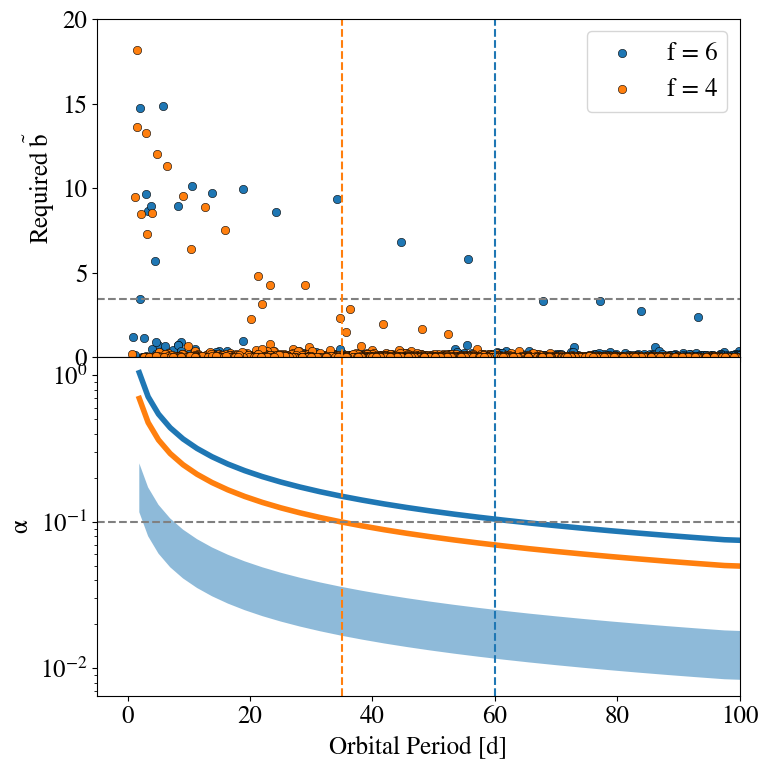
\includegraphics[width=0.5\textwidth]{figures/plStip/f6f4_b.png}
    \caption{In the top panel, we show the required feeding zone sizes to produce the masses of the bodies seen
    at the end of the fdHi and fdHif4 simulations.  The bottom panel shows the variation of $\alpha$ with orbital period for the 
    bodies used in each case (solid curves). The orbital period at which $\alpha \simeq 0.1$ matches well with the location at 
    which $\tilde{b}$ exceeds $2 \sqrt{3}$ This is highlighted by the vertical dashed lines. The shaded region
    in the bottom panel show the values of alpha for realistic-sized ($f=1$) planetesimals with bulk densities between 10 and 1 g cm$^{-3}$.\label{fig:f6f4_b}}
\end{center}
\end{figure}

\subsection{Collision Model}

\begin{figure}
\begin{center}
    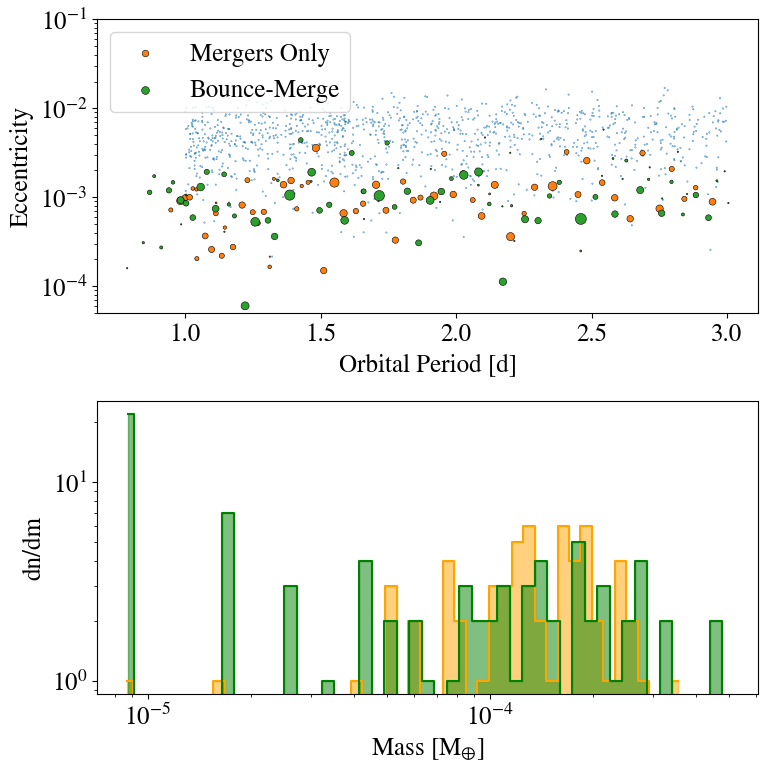
\includegraphics[width=0.5\textwidth]{figures/plStip/frag_ecc.png}
    \caption{A comparison between the innermost region of the fdLo (orange) simulation, and a second version using a bounce-
    merge collision model (green). In the top panel, the period-eccentricity state of the particles is shown, with marker sizes 
    indicating relative mass. The blue points represent the initial state of the simulations. The bottom panel compares the final 
    differential mass distributions of the bodies. \label{fig:frag_ecc}}
\end{center}
\end{figure}

\begin{figure}
\begin{center}
    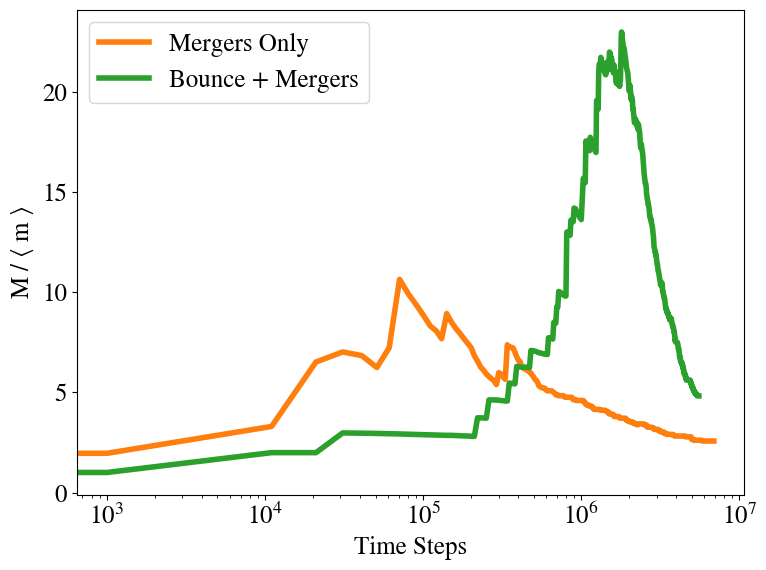
\includegraphics[width=0.5\textwidth]{figures/plStip/frag_evo.png}
    \caption{The evolution of the ratio between the maximum and mean mass of the simulations shown in figure \ref{fig:frag_ecc}. 
    In both cases, the system first evolves through a phase of runaway growth, before the massive bodies consume the smaller 
    bodies, driving down the mean mass. With the bounce-merge model, the mass ratio takes much longer to begin decreasing.\label{fig:frag_evo}}
\end{center}
\end{figure}

For the simulations presented in this work, every collision results in a perfect merger between pairs of bodies, with no loss
of mass or energy. Although simpler and less computationally expensive to model, allowing every collision to produce a
perfect merger might result in overly efficient growth, particularly in the innermost region of the disk where the encounter 
velocities are largest. Given that we have just shown that a distinctly non-oligarchic growth mode emerges in the inner disk when the 
collision timescale is short relative to the gravitational scattering timescale, one might be concerned that a more realistic collision model would act 
to lengthen the growth timescale enough for this condition to no longer be true. In the outer regions of the disk where oligarchic growth still 
operates, more realistic collision models have been shown to simply lengthen the timescale for planetary embryos to form 
\cite{wetherill93, leinhardt05}. A proper way to handle this would be to allow for a range of collision outcomes, based on a semianalytic 
model (see \cite{leinhardt12}). However, resolving collisional debris, or even prolonging growth by forcing high-velocity pairs of 
bodies to bounce is too expensive to model, even with {\sc ChaNGa}.

To test whether a more restrictive collision model should alter the growth mode of the inner disk, we ran a smaller scale test 
using a more restrictive collision model. In this case, a collision can result in one of two outcomes: if the impact velocity is 
smaller than the mutual escape velocity of the colliding particles, defined as
\begin{equation}\label{eq:v_mut}
	v_{mut, esc} = \sqrt{\frac{2 G (m_{1} + m_{2})}{r_{1} + r_{2}}},
\end{equation}
where $m_{1}, m_{2}$ and $r_{1}, r_{2}$ are the masses and radii of
colliding particles 1 and 2, then the bodies merge. For
impact velocities larger than $v_{mut, esc}$, no mass is transferred, and the bodies undergo a completely elastic bounce. 
Because the accretion outcome is all or nothing, this model should restrict growth more than a partial accretion model 
\cite{leinhardt12}. Below, we will show that the bounce-merge model does not meaningfully affect the outcome of the inner 
disk's planetesimal accretion phase, and so a more realistic partial accretion model should do the same.

To compare the outcome of the two collision models, we have chosen to use the initial conditions from the fdLo simulation, but 
have truncated the disk beyond 3 days in orbital period. This offsets the increased computational cost of the more restrictive collision model, while still allowing the disk to evolve in the region where mergers would be most difficult to achieve.
For the initial conditions we have chosen, the typical encounter velocity (defined by $v_{enc} = \left< e^{2} \right>^{1/2} v_{k}$, 
where $v_{k}$ is the local Keplerian velocity) is about 25 percent larger than $v_{mut, esc}$. Because the encounter velocities 
follow a Gaussian distribution, there should still be a small subset of collisions that still meet the merger criteria to occur early on. 
In addition, $v_{mut, esc}$ becomes larger as the bodies grow and the merger criteria should become easier to meet as the 
system evolves. For these reasons, one would expect the inhibition of growth due to the more restrictive collision model to be 
temporary.

In figure \ref{fig:frag_ecc}, we compare the outcomes of the simulations, one with mergers only (shown in orange) and one with 
the bounce-merge model (shown in green). The blue points in the top panel show the initial conditions used for both cases. 
Although the bounce-merge simulation takes much longer to reach the same phase of evolution, the resulting orbital properties
are indistinguishable from the merger-only case. Performing a Kolmogrov-Smirnov test on the two mass distributions yields
a p-value of $2 \times 10^{-5}$, which tells us that the two mass distributions are quite firmly statistically different. If we remove
the initial mass planetesimals, a KS test yields a p-value of 0.1. We conclude that the embryo populations are nearly indistinguishable,
while the bounce-merge model produces a small amount of residual planetesimals.

To investigate the differences in growth between the two collision models early on, we show the time evolution of the ratio 
between the maximum and mean mass in figure \ref{fig:frag_evo}. In both cases, this ratio first increases, which indicates that 
runaway growth still operates, regardless of the collision model used. In the bounce-merge case, the mass ratio peaks at a 
higher value, while also undergoing a longer runaway growth phase. This suggests that the mass distribution becomes much 
less unimodal during this growth process, but as figure \ref{fig:frag_ecc} shows, this does not affect the resulting embryos or 
allow for a residual planetesimal population.

As a final note, \cite{childs22} found that a more realistic collision model also enhanced radial mixing in their simulations. Upon 
calculating the planetesimal accretion zones using the same method as was done to produce figure \ref{fig:acc_zones}, we find 
that the embryos in the bounce-merge simulation annulus do have modestly wider accretion zones than those produced in the 
merger-only simulation.

\section{Summary and Discussion} \label{sec:pl_stip_discuss}

In this work, we have demonstrated that planetary embryo growth
can simultaneously operate in two distinct modes in a planet-forming disk. In the first
mode, gravitational feedback from the growing embryos heats the
remaining planetesimals and results in a dynamically cold population
of embryos with a modest amount of residual planetesimals. This
corresponds to the ``oligarchic growth'' case revealed by \cite{kokubo98}, which is often used as a starting point for late-stage 
accretion models (e.g. \cite{kokubo02, raymond05, raymond06}). In the second mode, the gravitational feedback does not 
play a significant role, embryos quickly sweep up all planetesimals, and grow larger and less uniformly spaced than those produced by 
oligarchic growth.

We have demonstrated the outcome of both accretion modes through a
simple parameter study using a narrow annulus of planetesimals (section \ref{sec:narrow}). The initial planetesimal distribution can be described in terms of two dimensionless 
constants, $\alpha$ and $\beta$, which describe the ratio between the physical radius of the planetesimals and the Hill ($r_{h}$) 
and gravitational ($r_{g}$) radius, respectively. For a fixed planetesimal composition, $\alpha$ scales with the orbital period and 
$\beta$ scales with the level of dynamical excitation of the disk. We showed that $\alpha \ll 1$ leads to oligarchic growth, while an $\alpha$ close to unity produces this newly revealed non-oligarchic growth mode (see figure \ref{fig:alpha_beta}). Within this non-oligarchic mode, we find that 
the resulting masses and eccentricities of the embryos come out very similar, regardless of the initial value of $\beta$.

So long as the density of the bodies do not significantly change as
their mass distribution evolves, this ratio is set entirely by the distance
from the star. Because both the physical and Hill radii of the bodies
grows as $M^{1/3}$, the growth mode boundary remains stationary
 in the disk during the planetesimal accretion process.
 
We have verified that the growth boundary location does not strongly depend of the
solid surface density distribution by testing the outcome of the planetesimal
accretion process for a variety of solid
profiles. Although altering the surface density does affect the
resulting masses of the embryos, the location of the boundary
separating the growth modes is remarkably similar among all of our simulations.
In addition, the sizes of the feeding zones, along with qualitative differences in the
accretion history of embryos on both sides of the boundary (see figures \ref{fig:minor_frac} and \ref{fig:acc_zones}) provide further evidence to
suggest that oligarchic growth is not operating in the inner disk.

Finally, we have examined how our assumption of perfect accretion, along with the collision cross section enhancement used, might alter our results. 
We verified that these modifications, meant to make the simulations less computationally expensive, would still allow for the emergence of this 
non-oligarchic growth mode.
We showed that a much more restrictive collision model, in which only low-velocity collisions produce a merger, still allows for 
this growth mode to occur at the innermost part of the disk, where encounter speeds are most vigorous. In a real planet-forming 
disk, partial accretion events should allow growth to happen more quickly than what was seen in this test case (see figure 8 of \cite{leinhardt15}), so this growth 
mode should certainly still occur. We also showed that the collision cross section enhancement moves the accretion boundary 
outward. We verified this by deriving a scaling relation between the boundary location and the bulk density of the planetesimals, 
and showing that the boundary moves to the predicted location when running a simulation with a slightly smaller inflation factor. 
For rocky planetesimals with a realistic bulk density, 3 g cm$^{-3}$, our results suggest that this boundary should lie around 5 days in orbital period.

\subsection{Connections to Satellitesimal Accretion}

To date, there have been no other studies of planetesimal accretion
with such a large value of $\alpha$. Typically, it is assumed that $\alpha \ll 1$ (e.g. \cite{lithwick14}), which is certainly true for material at and beyond the Earth's orbit. However, a value of $\alpha = 1$
corresponds to the Roche limit of a three-body system, and so one
might wonder this high-$\alpha$ accretion mode might be relevant for a
circumplanetary accretion. There is a collection of previous works
which use N-body methods to examine in-situ satellitesimal accretion
\cite{ida97, richardson00, kokubo00b, ida20}, although some of these simulations involve a complex interaction between spiral 
density waves formed inside of the Roche limit and the material exterior to it, making the dynamics driving accretion distinctly non-local, in contrast to what we have presented in this work. \cite{ida97} was able to form 1-2
large moons just exterior to the Roche limit, depending on the extent of the disk with very little satellitesimal material left over. 
The widest disk they modeled extended out to $\alpha = 0.5$. Qualitatively, this result is very similar to the short period 
planetesimal accretion mode observed in our simulations. \cite{ida20} modeled a much wider satellitesimal disk, which extends 
out to about $\alpha \approx 0.05$. Inside to the $\alpha = 0.1$ accretion boundary (which lies near 15 planetary radii in figure 1 of 
\cite{ida20}), bodies grow beyond the isolation mass, while the opposite is true on the other side of the boundary. In addition, a 
residual population of satellitesimals is still present beyond the boundary, which suggests that oligarchic growth is indeed 
operating only on the far side.

Presently, the implications that this non-oligarchic accretion mode has for the formation of short-period terrestrial planets, and 
whether the accretion boundary would leave any lasting imprint on the final orbital architecture, is unclear. The extreme efficiency of planetesimal accretion at the inner edge of the disk suggests that no residual populations of small bodies should be expected to exist here. A crucial point that our 
results do highlight is that the initial conditions used for most late-stage planet formation simulations are overly simplistic. 
\cite{clement20} recently simulated planetesimal accretion in a disk extending from the orbit of Mercury to the asteroid belt and 
found that the disk never reaches a state in which equally-spaced, isolation mass embryos are present everywhere 
simultaneously. Instead, different annuli reach a `giant impact' phase at different times, preventing the onset of a global instability 
throughout the entire disk, as is common in classic terrestrial planet formation models \cite{chambers01, raymond09}.

To connect these accretion modes to the final orbital architecture,
and to ultimately determine what implications an in-situ formation model has for the growth of STIPs, we will evolve the final 
simulation snapshots presented here with a hybrid-symplectic integrator for Myr timescales. The final distribution of planets 
formed, along with composition predictions generated by applying cosmochemical models to our initial planetesimal distributions 
and propagating compositions through the collision trees, will be examined in the following chapter.

\section{Robustness of Timestepping Scheme}\label{sec:rung_ecc}

As described in section \ref{sec:methods}, {\sc ChaNGa}
  evolves the motions of the particles in the planetesimal disk using
  a multi-tiered timestepping scheme. Due to the extremely short
  dynamical timescale at the inner edge of the disk, the outer disk
  would require a prohibitive number of timesteps to reach the
  protoplanet phase using a fixed timestep scheme.  To circumvent this, particles are evolved in discrete power-of-two timestep groups. In the event that a collision occurs between two particles on different timesteps, a slight error is introduced to the energy and angular momentum of the merged particle. Due to the nonlinear nature of the runaway growth phase, this slight error tends to trigger more subsequent collisions at the timestep boundary in the disk, and causes protoplanets to preferentially form at the boundaries.

To circumvent this issue, we prohibit particles on different timesteps from merging until the runaway growth phase is well underway. For the fdHi simulation, multi-tiered mergers are not allowed during the first thousand steps. To verify that this technique does not alter the resulting protoplanet distribution in any meaningful way, we ran two test simulations of the inner part (1 to 4 days in orbital period) of the disk from the fdHi simulation. In the first case, the aforementioned timestepping scheme is used. In the second case, all particles are evolved on the timestep appropriate for the inner edge of the disk.

\begin{figure}
\begin{center}
    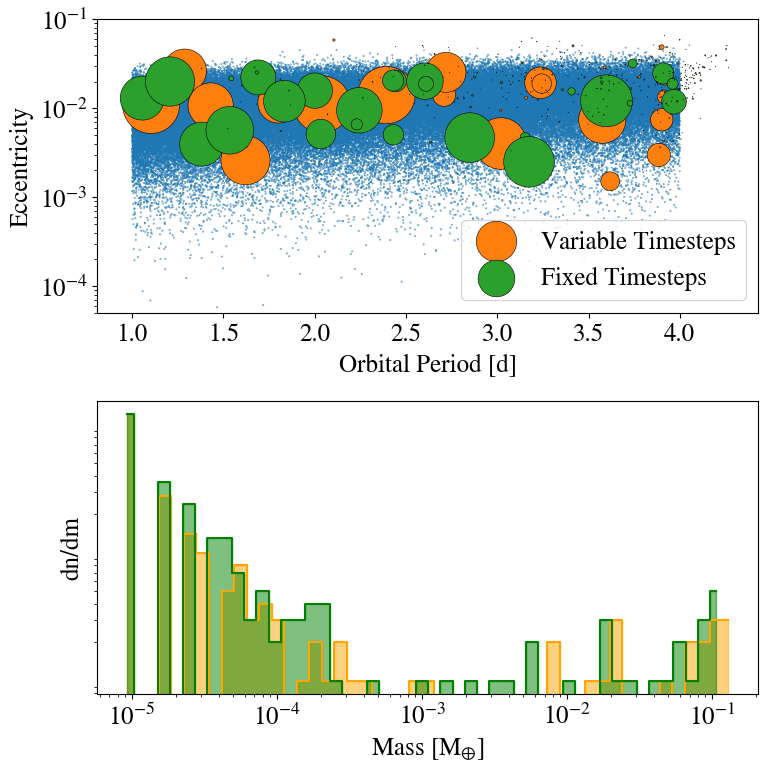
\includegraphics[width=0.5\textwidth]{figures/plStip/rung_ecc.png}
    \caption{A comparison between the innermost region of the fdHi (orange) simulation, and a second version using a fixed timestep appropriate for the inner edge of the disk (green). In the top panel, the period-eccentricity state of the particles is shown, with marker sizes indicating relative mass. The blue points represent the initial state of the simulations. The bottom panel compares the final mass distributions of the bodies.\label{fig:rung_ecc}}
\end{center}
\end{figure}

In figure \ref{fig:rung_ecc}, we compare the final period-eccentricity state and final mass distributions to each other. There do not appear to be any differences between the two protoplanet distributions, particularly near the timestep boundary at 2 days. In addition, the masses of both the protoplanets and the remaining growing planetesimals are indistinguishable. In this case, a KS test of the two mass distributions yields a p-value of $\sim 0.34$. We therefore safely conclude that the timestepping scheme used in this work does not alter the growth of the protoplanets in any meaningful way.
\chapter {In-Situ Formation of STIPs}

%Intro outline:
% What are STIPs, why important
% Outline of formation theories, migration vs in-situ
% Problems with migration models, in-situ simpler
% Outline my previous paper
% Motivation: does accretion boundary leave any imprint on final orbital arcitectures?

\section{Introduction} \label{sec:intro}

One of the most surprising and intriguging results from NASA's \textit{Kepler} mission was the prevalance 
of sub-Neptune-sized exoplanets with orbital periods shorter than that of Mercury \cite{borucki10}. These 
planets are often found in closely-spaced groups, known as systems of tightly-packed inner planets (
STIPs) \cite{latham11, lissauer11, lissauer14}. STIPs are found to often be coplanar 
\cite{fang12, tremaine12}, have low eccentricities \cite{vaneylen15, hadden17} and are usually not in 
mean-motion resonance with each other \cite{fabrycky14, steffen15}. In addition these systems have been 
shown to exhibit a compelling amount of uniformity between adjacent planets, in terms of mass, radius and 
orbital spacing \cite{millholland17, millholland21}.

All of these characteristics provide a rich set of constraints for planet formation models. One of the 
most intriguing questions that arises is why the structure of the present-day solar system appears so 
different than that of STIPs. Extending the minimum-mass solar nebular (MMSN) model \cite{hayashi81} down 
to $\sim$ 0.05 AU, where the inner edge of many protoplanetary disks are thought to be \cite{meyer97} (
and where planetesimals are thought to form \cite{mulders18}) yields several extra Earth masses of 
material. Explaining why this material is missing from the solar system, but not some exoplanetary 
systems, is a key question that a complete theory of planet formation must be able to provide.

There are two categories of formation theories mean to explain the ubiquity of these compact, short-period systems. The first involves the gradual assembly of these worlds as they migrate inwards.

% Text from NSF proposal:

%With the number of confirmed exoplanets now exceeding 4000, there is now a large enough statistical sample from which to test planet formation theories. The most striking trend in this sample is the prevalence of planets with orbital periods shorter than that of Mercury. Many of these planets come in closely-packed multiples \citep{2014ApJ...790..146F}, known as systems of tightly packed inner planets (STIPs). So far, nearly all STIPs have been found around M stars \citep{2015ApJ...807...45D}. Extending the minimum-mass solar nebula (MMSN) model \citep{1981PThPS..70...35H} down to $\approx$ 0.05 AU, where the inner edge of many protoplanetary disks are thought to be \citep{1997AJ....114..288M} yields several extra Earth masses of material. Explaining why this material is missing from the solar system, but not some exoplanetary systems, is a key question that a complete theory of planet formation must be able to explain.

%There are two categories of theories meant to explain the ubiquity of these compact, short period systems. The first involves the gradual assembly of these worlds as they migrate inwards. Bodies larger than Mars are expected to experience strong torques from the gas disk that drive a substantial amount of migration \citep{1997Icar..126..261W}. Unfortunately, the strength and even direction of this effect is highly uncertain and depends on the detailed physical structure of the disk, along with the specifics of the thermodynamic model used \citep{2010MNRAS.408..876A, 2013A&A...549A.124B}. In addition, many STIPs do not lie in resonant chains, which should be a generic result of convergent migration \citep{2014MNRAS.445..749H}, although dynamical instabilities \citep{2007ApJ...654.1110T, 2019arXiv190709313M} or even turbulence \citep{2011A&A...531A...5P} can potentially disrupt resonant chains after they form.

%Alternatively, these planets may have formed in situ, being constructed only from the local mass budget of the disk. This may be the case for the gaseous envelopes that hot Jupiters attain near the inner edge of the disk \citep{2018ApJ...866L...2B}, although it is not clear if the cores of these worlds also formed locally. Additionally, magnetically driven disk winds, which are especially prevalent around M stars, have been shown to flatten the radial surface density profile, which suppresses type I migration \citep{2018A&A...615A..63O}.

%One of the first simulations of in situ short period terrestrial planet accretion was done by \citet{2007ApJ...669..606R}, who concluded that it was extremely difficult for this process to occur near the habitable zone of M stars. However, the initial conditions used were based off of the MMSN, scaled linearly by the mass of the host star. \citet{2013MNRAS.431.3444C} later showed that the rescaled MMSN tends to underpredict the mass budget of many extrasolar disks. Starting with a much higher surface density, \citet{2012ApJ...751..158H} were able to produce short period Earth-sized planets without invoking migration. A subsequent study by \citet{2014ApJ...795L..15S} argued that applying the MMSN analysis to some exoplanetary systems produced disks that were unphysical, assuming a gas to dust ratio of 1\%. There is no evidence, however that this ratio is universal and there is mounting evidence that shows that this quantity can vary radially \citep{2012ApJ...744..162A, 2014ApJ...788...59W}. It should also be noted that as of yet there are no direct measurements of the surface density profiles of the inner parts of protoplanetary disks. Additionally, the dust masses of disks measured with ALMA have been shown to sometimes underpredict the true values \citep{2019ApJ...878..116P, 2019ApJ...877L..18Z}.

%The question of whether or not in situ formation is viable for STIPs seems to rest largely on what the distribution of planetary embryos looked like that went on to assemble the final configuration of planets. In all of the aforementioned studies, the oligarchic growth model \citep{1998Icar..131..171K, 2000Icar..143...15K} is used to predict the sizes and spacings between the embryos going into the final phase of accretion. \citet{2002ApJ...581..666K} explored the influence of planetesimal orbital distance and surface density profile on the distribution of embryos, but did not extend the search of parameter space down to be of relevance to most STIPs.

%As we will present in a pilot study, runaway and oligarchic growth, which produces a bimodal population of embryos and dynamically hot, difficult to accrete planetesimals, does not appear to operate at short orbital periods. With a colder background population of planetesimals, growth should be more efficient and result in larger embryos. More massive embryos are also less affected by radial drift, which has been cited as a problem with short period in situ formation models \citep{2015MNRAS.448.1751I}. Given the lack of work that has been done on short period planetesimal accretion, along with the subsequent discovery that short period terrestrial worlds are incredibly common, a more careful examination of this phase of growth is warranted. This will place better context on the initial conditions used by recent simulations of short period late stage accretion.

\chapter {Summary and Future Work}

% TODO: Plot of particle count vs publication date

\section{Summary}
The purpose of this dissertation has been to bridge the gap between planetesimal formation and the final assembly of terrestrial planets. As discussed in section \ref{sec:obsConstraints}, the observational markers of this phase of the planet formation processes are subtle and unlikely to be detectable in the present and near-future. For this reason, simulations will remain the most promising way forward. Due to the bottom-up nature of terrestrial planet growth, the number of particles that must be modeled as one goes back in time grows prohibitively large, particularly with an N-body approach. Using our state-of-the-art N-body code {\sc ChaNGa},we self-consistently follow the growth and orbital evolution of solid bodies from planetesimals to full-sized terrestrial planets for the first time.

Along the way, I reveal some shortcomings of previous planetesimal accretion and planet formation models that largely stem from prior computational constraints. In chapter \ref{ch:plSS}, I showed that the planetsimal accretion process itself is size-dependent. During the oligarchic growth phase, mean motion resonances with the largest bodies become populated by plantesimals, which shortens the timescale for energy equipatition, altering the growth mode and producing a broken power-law size distribution. This only occurs if the particle resolution is sufficiently fine-grained and is expected to operate for 100 km-sized and smaller bodies predicted by plantesimal formation models. I show that the exact location of the break depends on the initial planetesimal size and that the size distribution of the remaining small body populations in the solar system could potentially be used to constrain planetesimal formation mechanisms.

In chapter \ref{ch:grind}, I map out the collisional structure of a planetesimal belt perturbed by mean-motion resonances with a giant planet. After mapping the radial collision function to expected dust emission, I show that the presence of bright rings or gaps near the locations of resonances can be used to constrain the mass and eccentricity of the planet. This structure in the dust emission depends on interactions between planetesimals near the edges of the resonances and is only produceable if the simulated planetesimals are of near-realistic sizes.

Finally, in chapter \ref{ch:stipPl}, I use the incredible resolution afforded by {\sc ChaNGa} to follow the planetesimal growth process across a disk of solids spanning two orders of magnitude in orbital period, again starting from near-realistic sizes. At short orbital periods, energy equipartition becomes ineffective and oligarchic growth does not operate. This produces a boundary between accretion modes in the disk and breaks the self-similarity of the planetary embryo formation process, which is a common assumption used in terrestrial planet formation simulations. In chapter \ref{ch:stipFinal}, I pass the results of these simulations to a hybrid mixed-variable symplectic code to follow the planet growth process to completion. After doing so, I use the simulation snapshots to map the initial locations of planetesimals to the eventual planets that form and show that a migration-free terrestrial planet formation model produces a significant amount of radial mixing of material. In addition, I train a neural network to generate a much larger set of post-{\sc ChaNGa} snapshots and run these to completion. This provides a statistical sample from which I measure the planet occurrence rate as a function of orbital period. Similar to the occurrence rate measured by Kepler, my simulations produce a power law break around $\sim$ 10 days, which suggests that a large fraction of compact multiplanet systems may have formed in-situ.

\section{Future Work: Understanding the Behavior of Planetesimal-Driven Migration}

The migration history of a planet and its building blocks play a key role in determining its final composition, the eventual makeup of its atmosphere, and even its ability to harbor life. Up to this point in time, migration models have mainly focused on gas disk-driven interactions. Although this mechanism can play a definitive role in shaping the architectures of both terrestrial and gas giant systems, its influence only lasts for a small fraction of the planet-building phase, largely ending within the first few Myr. Beyond this point, migration can continue via weak but numerous gravitational interactions between the protoplanets and remaining planetesimals. This mechanism, known as planetesimal-driven migration (PDM), appears to have played a pivotal role in shaping the structure of the solar system \cite{tsiganis05, levison11, nesvorny11}, has been invoked to explain the near-resonant pairs of planets observed by Kepler \cite{chatterjee15}, and even has the potential to counteract gas disk migration \cite{minton14}. Despite the wide range of scenarios in which PDM is invoked, its behavior remains largely unexplored and has not yet been incorporated into any planetary population synthesis models. 

Much of this lack of attention to PDM stems from the fact that planetesimal interactions are often ignored in planet formation simulations due to computational expense. As I have shown in my thesis, dynamical interactions involving planetesimals also require sufficient resolution to properly operate. Compared to gas disk-driven migration, PDM requires far fewer modeling assumptions and is not directly coupled to the thermodynamic properties of the disk. For this reason, a thorough investigation of PDM using high resolution N-body simulations is a necessary step to fully understand the processes that transport solids throughout a planet-forming disk.

\section{Future Work: Pathways to Instability in Systems of Protoplanets}

In the standard picture of terrestrial planet formation, the final coalescence of protoplanets is typically delayed by the presence of gas in the disk. Where oligarchic growth operates, protoplanets stall at the `isolation mass'. Aerodynamic drag and gas dynamical friction prevent the protoplanets from \textbf{undergoing a large-scale gravitational instability that perturbs them} onto crossing orbits and \textbf{instigates the collisions which} form larger bodies. Because growth beyond a Mars mass is suspended while the protoplanetary gas is present, the planets that form in this region should fail to acquire a significant hydrogen envelope. While this delayed assembly picture is consistent with the properties of the inner solar system planets, recently discovered super-Earth and hot Jupiter systems require a more complicated explanation, often invoking migration.

Despite the crucial role that this delayed assembly model plays, the behavior and timing of the instability itself remains poorly understood. In cases where the gas and dust profile in the disk is non-monotonic, the instability could trigger only in select locations and spread to regions where substantial amounts of gas are still present. Studying this problem in more detail could be key to explaining a wide range of observational features, such as the radius gap \cite{fulton17}, bulk density measurements \cite{lopez14, wolfgang15} and atmospheric composition measurements by JWST.

In most cases, a smoothly varying `minimum mass solar nebula' (MMSN) disk model is used (e.g. \cite{kominami02, dawson15}), which triggers the instability everywhere once the gas density sufficiently decays. However, a MMSN model is not compatible with many exoplanetary systems \cite{chiang13, schlichting14}. As I showed in chapter \ref{ch:stipPl}, a smooth distribution of planetesimals does not always produce a smooth distribution of protoplanets. Furthermore, non-monotonic gas profiles are being invoked in protoplanetary disk models \cite{chatterjee14, ogihara15} and are even supported by observations of nearby disks with ALMA \cite{isella16, andrews16}. For these cases, the instability might trigger only in special places in the disk and could even spread to regions where substantial amounts of gas are still present. If protoplanetary cores in the terrestrial region can grow large enough to accrete gas before photoevaporation from the central star removes the majority of it, the need for migration in formation models for super-Earths and hot Jupiters would be greatly reduced.

% TODO: Final summary of future work to close things off

%
% ==========   Bibliography
%
\nocite{*}   % include everything in the uwthesis.bib file
\bibliographystyle{plain}
\bibliography{uwthesis}


\end{document}
